%%**************************************************************
%% Vorlage fuer Bachelorarbeiten (o.ä.) der DHBW
%%
%% Autor: Tobias Dreher, Yves Fischer
%% Datum: 06.07.2011
%%
%% Autor: Michael Gruben
%% Datum: 15.05.2013
%%
%% Autor: Markus Barthel
%% Datum: 22.08.2014
%%**************************************************************

%!TEX root = ../dokumentation.tex

%
% Nahezu alle Einstellungen koennen hier getaetigt werden
%

\RequirePackage[l2tabu, orthodox]{nag}	% weist in Commandozeile bzw. log auf veraltete LaTeX Syntax hin

\documentclass[%
	pdftex,
	oneside,			% Einseitiger Druck.
	12pt,				% Schriftgroesse
	parskip=half,		% Halbe Zeile Abstand zwischen Absätzen.
	%	topmargin = 10pt,	% Abstand Seitenrand (Std:1in) zu Kopfzeile [laut log: unused]
	headheight = 12pt,	% Höhe der Kopfzeile
	%	headsep = 30pt,	% Abstand zwischen Kopfzeile und Text Body [laut log: unused]
	headsepline,		% Linie nach Kopfzeile.
	footsepline,		% Linie vor Fusszeile.
	footheight = 16pt,	% Höhe der Fusszeile
	abstracton,		% Abstract Überschriften
	DIV=calc,		% Satzspiegel berechnen
	BCOR=8mm,		% Bindekorrektur links: 8mm
	headinclude=false,	% Kopfzeile nicht in den Satzspiegel einbeziehen
	footinclude=false,	% Fußzeile nicht in den Satzspiegel einbeziehen
	listof=totoc,		% Abbildungs-/ Tabellenverzeichnis im Inhaltsverzeichnis darstellen
	toc=bibliography,	% Literaturverzeichnis im Inhaltsverzeichnis darstellen
]{scrreprt}	% Koma-Script report-Klasse, fuer laengere Bachelorarbeiten alternativ auch: scrbook

% Einstellungen laden
\usepackage{xstring}
\usepackage[utf8]{inputenc}
\usepackage[T1]{fontenc}

\newcommand{\einstellung}[1]{%
	\expandafter\newcommand\csname #1\endcsname{}
	\expandafter\newcommand\csname setze#1\endcsname[1]{\expandafter\renewcommand\csname#1\endcsname{##1}}
}
\newcommand{\langstr}[1]{\einstellung{lang#1}}

\einstellung{titel}
\einstellung{datumAbgabe}
\einstellung{firma}
\einstellung{firmenort}
\einstellung{abgabeort}
\einstellung{abschluss}
\einstellung{studiengang}
\einstellung{dhbw}
\einstellung{betreuer}
\einstellung{gutachter}
\einstellung{zeitraum}
\einstellung{arbeit}
\einstellung{sprache}
\einstellung{schriftart}
\einstellung{seitenrand}
\einstellung{kapitelabstand}
\einstellung{spaltenabstand}
\einstellung{zeilenabstand}
\einstellung{zitierstil}

% student 1
\einstellung{kurs}
\einstellung{autor}
\einstellung{martrikelnr}

% student 2
\einstellung{kursb}
\einstellung{autorb}
\einstellung{martrikelnrb} % verfügbare Einstellungen
%%%%%%%%%%%%%%%%%%%%%%%%%%%%%%%%%%%%%%%%%%%%%%%%%%%%%%%%%%%%%%%%%%%%%%%%%%%%%%%
% Einstellungen
%
% Hier können alle relevanten Einstellungen für diese Arbeit gesetzt werden.
% Dazu gehören Angaben u.a. über den Autor sowie Formatierungen.
%
%
%%%%%%%%%%%%%%%%%%%%%%%%%%%%%%%%%%%%%%%%%%%%%%%%%%%%%%%%%%%%%%%%%%%%%%%%%%%%%%%


%%%%%%%%%%%%%%%%%%%%%%%%%%%%%%%%%%%% Sprache %%%%%%%%%%%%%%%%%%%%%%%%%%%%%%%%%%%
%% Aktuell sind Deutsch und Englisch unterstützt.
%% Es werden nicht nur alle vom Dokument erzeugten Texte in
%% der entsprechenden Sprache angezeigt, sondern auch weitere
%% Aspekte angepasst, wie z.B. die Anführungszeichen und
%% Datumsformate.
\setzesprache{en} % oder en
%%%%%%%%%%%%%%%%%%%%%%%%%%%%%%%%%%%%%%%%%%%%%%%%%%%%%%%%%%%%%%%%%%%%%%%%%%%%%%%%

%%%%%%%%%%%%%%%%%%%%%%%%%%%%%%%%%%% Angaben %%%%%%%%%%%%%%%%%%%%%%%%%%%%%%%%%%%
%% Die meisten der folgenden Daten werden auf dem
%% Deckblatt angezeigt, einige auch im weiteren Verlauf
%% des Dokuments.

% student 1
\setzemartrikelnr{XXXXXXX}
\setzekurs{XXXXXXX}
\setzeautor{Nguyen Viet Do}

% student 2
\setzemartrikelnrb{XXXXXXX}
\setzekursb{XXXXXXX}
\setzeautorb{Nico Vogel}

\setzetitel{Analysis and evaluation of NodeJS microservice technologies for an exemplary LAN-Party management application}
%\setzetitel{Logfileanalyse mit Apache{\textsuperscript{TM}} Hadoop\textsuperscript{{\textregistered}} MapReduce}
\setzedatumAbgabe{June 2020}
\setzefirma{nothing}
\setzefirmenort{nothing}
\setzeabgabeort{Stuttgart}
\setzeabschluss{nothing}
\setzestudiengang{Informatik}
\setzedhbw{Stuttgart}
\setzebetreuer{XXXXXXX XXXXXXX}
\setzegutachter{nothing}
\setzezeitraum{10/09/2020-06/08/2020}
\setzearbeit{Studienarbeit}
%%%%%%%%%%%%%%%%%%%%%%%%%%%%%%%%%%%%%%%%%%%%%%%%%%%%%%%%%%%%%%%%%%%%%%%%%%%%%%%%

%%%%%%%%%%%%%%%%%%%%%%%%%%%% Literaturverzeichnis %%%%%%%%%%%%%%%%%%%%%%%%%%%%%%
%% Bei Fehlern während der Verarbeitung bitte in ads/header.tex bei der
%% Einbindung des Pakets biblatex (ungefähr ab Zeile 110,
%% einmal für jede Sprache), biber in bibtex ändern.
\newcommand{\ladeliteratur}{%
	\addbibresource{bibliography.bib}
	%\addbibresource{weitereDatei.bib}
}
%% Zitierstil
%% siehe: http://ctan.mirrorcatalogs.com/macros/latex/contrib/biblatex/doc/biblatex.pdf (3.3.1 Citation Styles)
%% mögliche Werte z.B numeric-comp, alphabetic, authoryear
\setzezitierstil{numeric-comp}
%%%%%%%%%%%%%%%%%%%%%%%%%%%%%%%%%%%%%%%%%%%%%%%%%%%%%%%%%%%%%%%%%%%%%%%%%%%%%%%%

%%%%%%%%%%%%%%%%%%%%%%%%%%%%%%%%% Layout %%%%%%%%%%%%%%%%%%%%%%%%%%%%%%%%%%%%%%%
%% Verschiedene Schriftarten
% laut nag Warnung: palatino obsolete, use mathpazo, helvet (option scaled=.95), courier instead
\setzeschriftart{lmodern} % palatino oder goudysans, lmodern, libertine

%% Paket um Textteile drehen zu können
%\usepackage{rotating}
%% Paket um Seite im Querformat anzuzeigen
%\usepackage{lscape}

%% Seitenränder
\setzeseitenrand{2.5cm}

%% Abstand vor Kapitelüberschriften zum oberen Seitenrand
\setzekapitelabstand{20pt}

%% Spaltenabstand
\setzespaltenabstand{10pt}
%%Zeilenabstand innerhalb einer Tabelle
\setzezeilenabstand{1.5}
%%%%%%%%%%%%%%%%%%%%%%%%%%%%%%%%%%%%%%%%%%%%%%%%%%%%%%%%%%%%%%%%%%%%%%%%%%%%%%%%

%%%%%%%%%%%%%%%%%%%%%%%%%%%%% Verschiedenes %%%%%%%%%%%%%%%%%%%%%%%%%%%%%%%%%%%
%% Farben (Angabe in HTML-Notation mit großen Buchstaben)
\newcommand{\ladefarben}{%
	\definecolor{LinkColor}{HTML}{00007A}
	\definecolor{ListingBackground}{HTML}{FCFAFB}
}
%% Mathematikpakete benutzen (Pakete aktivieren)
\usepackage{amsmath}
\usepackage{amssymb}

%% Programmiersprachen Highlighting (Listings)
\newcommand{\listingsettings}{%
	\lstset{%
		language=Java,			% Standardsprache des Quellcodes
		numbers=left,			% Zeilennummern links
		stepnumber=1,			% Jede Zeile nummerieren.
		numbersep=5pt,			% 5pt Abstand zum Quellcode
		numberstyle=\tiny,		% Zeichengrösse 'tiny' für die Nummern.
		breaklines=true,		% Zeilen umbrechen wenn notwendig.
		breakautoindent=true,	% Nach dem Zeilenumbruch Zeile einrücken.
		postbreak=\space,		% Bei Leerzeichen umbrechen.
		tabsize=2,				% Tabulatorgrösse 2
		basicstyle=\ttfamily\footnotesize, % Nichtproportionale Schrift, klein für den Quellcode
		showspaces=false,		% Leerzeichen nicht anzeigen.
		showstringspaces=false,	% Leerzeichen auch in Strings ('') nicht anzeigen.
		extendedchars=true,		% Alle Zeichen vom Latin1 Zeichensatz anzeigen.
		captionpos=b,			% sets the caption-position to bottom
		backgroundcolor=\color{ListingBackground}, % Hintergrundfarbe des Quellcodes setzen.
		xleftmargin=0pt,		% Rand links
		xrightmargin=0pt,		% Rand rechts
		frame=single,			% Rahmen an
		frameround=ffff,
		rulecolor=\color{darkgray},	% Rahmenfarbe
		fillcolor=\color{ListingBackground},
		keywordstyle=\color[rgb]{0.133,0.133,0.6}\bfseries,
		commentstyle=\color{Sepia},
		stringstyle=\color{red}
	}
}
%%%%%%%%%%%%%%%%%%%%%%%%%%%%%%%%%%%%%%%%%%%%%%%%%%%%%%%%%%%%%%%%%%%%%%%%%%%%%%%%

%%%%%%%%%%%%%%%%%%%%%%%%%%%%%%%% Eigenes %%%%%%%%%%%%%%%%%%%%%%%%%%%%%%%%%%%%%%%
%% Hier können Ergänzungen zur Präambel vorgenommen werden (eigene Pakete, Einstellungen)

% xcolor muss mit optionen vor pdfpages geladen werden
\usepackage[usenames,dvipsnames,table,xcdraw]{xcolor} 	%xcolor für HTML-Notation

\usepackage{pdfpages}

\usepackage{xargs}
\usepackage[colorinlistoftodos,prependcaption,textsize=tiny]{todonotes}
\newcommandx{\unsure}[2][1=]{\todo[linecolor=red,backgroundcolor=red!25,bordercolor=red,#1]{#2}}
\newcommandx{\change}[2][1=]{\todo[linecolor=blue,backgroundcolor=blue!25,bordercolor=blue,#1]{#2}}
\newcommandx{\info}[2][1=]{\todo[linecolor=OliveGreen,backgroundcolor=OliveGreen!25,bordercolor=OliveGreen,#1]{#2}}
\newcommandx{\improvement}[2][1=]{\todo[linecolor=Plum,backgroundcolor=Plum!25,bordercolor=Plum,#1]{#2}}

 % lese Einstellungen

\newcommand{\iflang}[2]{%
	\IfStrEq{\sprache}{#1}{#2}{}
}

\langstr{abkverz}
\langstr{anhang}
\langstr{glossar}
\langstr{deckblattabschlusshinleitung}
\langstr{artikelstudiengang}
\langstr{studiengang}
\langstr{anderdh}
\langstr{von}
\langstr{dbbearbeitungszeit}
\langstr{dbname}
\langstr{dbmatriknr}
\langstr{dbkurs}
\langstr{dbfirma}
\langstr{dbbetreuer}
\langstr{dbgutachter}
\langstr{sperrvermerk}
\langstr{erklaerung}
\langstr{abstract}
\langstr{listingname}
\langstr{listlistingname}
\langstr{listingautorefname}
 % verfügbare Strings
\input{lang/\sprache} % Übersetzung einlesen

% Einstellung der Sprache des Paketes Babel und der Verzeichnisüberschriften
\iflang{de}{\usepackage[english, ngerman]{babel}}
\iflang{en}{\usepackage[ngerman, english]{babel}}


%%%%%%% Package Includes %%%%%%%

\usepackage[margin=\seitenrand,foot=1cm]{geometry}	% Seitenränder und Abstände
\usepackage[activate]{microtype} %Zeilenumbruch und mehr
\usepackage[onehalfspacing]{setspace}
\usepackage{makeidx}
\usepackage[autostyle=true,german=quotes]{csquotes}
\usepackage{tabularx}
\usepackage{longtable}
\usepackage{multirow}
\usepackage{enumitem}	% mehr Optionen bei Aufzählungen
\usepackage{graphicx}
%\usepackage[usenames,dvipsnames,table,xcdraw]{xcolor} 	%xcolor für HTML-Notation
\usepackage{float}
\usepackage{array}
\usepackage{calc}		% zum Rechnen (Bildtabelle in Deckblatt)
\usepackage[right]{eurosym}
\usepackage{wrapfig}
\usepackage{pgffor} % für automatische Kapiteldateieinbindung
\usepackage[perpage, hang, multiple, stable]{footmisc} % Fussnoten
%\usepackage[nohyperlinks]{acronym} % falls gewünscht kann die Option footnote eingefügt werden, dann wird die Erklärung nicht inline sondern in einer Fußnote dargestellt
\usepackage{acronym}

\usepackage{listings}

% Eigene zusätzliche packages
\usepackage{xfrac}
\usepackage{tikz}
\usepackage{subcaption}
%\usepackage[leqno]{amsmath}
%\usepackage{remreset}

% Wurzel mit schießendem Strich am ende
% New definition of square root: % it renames \sqrt as \oldsqrt
\let\oldsqrt\sqrt % it defines the new \sqrt in terms of the old one 
\def\sqrt{\mathpalette\DHLhksqrt} \def\DHLhksqrt#1#2{
	\setbox0=\hbox{$#1\oldsqrt{#2\,}$}\dimen0=\ht0 \advance\dimen0-0.2\ht0 \setbox2=\hbox{\vrule height\ht0 depth -\dimen0}{\box0\lower0.4pt\box2}}

%\makeatletter
%\@removefromreset{equation}{chapter}
%\makeatother
%\renewcommand*{\theequation}{\arabic{equation}}

% eine Kommentarumgebung "k" (Handhabe mit \begin{k}<Kommentartext>\end{k},
% Kommentare werden rot gedruckt). Wird \% vor excludecomment{k} entfernt,
% werden keine Kommentare mehr gedruckt.
\usepackage{comment}
\specialcomment{k}{\begingroup\color{red}}{\endgroup}
%\excludecomment{k}


%%%%%% Configuration %%%%%

%% Anwenden der Einstellungen

\usepackage{\schriftart}
\ladefarben{}

% Titel, Autor und Datum
\title{\titel}
\author{\autor}
\date{\datum}

% PDF Einstellungen
\usepackage[%
	pdftitle={\titel},
	pdfauthor={\autor},
	pdfsubject={\arbeit},
	pdfcreator={pdflatex, LaTeX with KOMA-Script},
	pdfpagemode=UseOutlines, 		% Beim Oeffnen Inhaltsverzeichnis anzeigen
	pdfdisplaydoctitle=true, 		% Dokumenttitel statt Dateiname anzeigen.
	pdflang={\sprache}, 			% Sprache des Dokuments.
]{hyperref}

% (Farb-)einstellungen für die Links im PDF
\hypersetup{%
	colorlinks=true, 		% Aktivieren von farbigen Links im Dokument
	linkcolor=LinkColor, 	% Farbe festlegen
	citecolor=LinkColor,
	filecolor=LinkColor,
	menucolor=LinkColor,
	urlcolor=LinkColor,
	linktocpage=true, 		% Nicht der Text sondern die Seitenzahlen in Verzeichnissen klickbar
	bookmarksnumbered=true 	% Überschriftsnummerierung im PDF Inhalt anzeigen.
}
% Workaround um Fehler in Hyperref, muss hier stehen bleiben
\usepackage{bookmark} %nur ein latex-Durchlauf für die Aktualisierung von Verzeichnissen nötig

% Schriftart in Captions etwas kleiner
\addtokomafont{caption}{\small}

% Literaturverweise (sowohl deutsch als auch englisch)
\iflang{de}{%
	\usepackage[
		backend=bibtex,		% empfohlen. Falls biber Probleme macht: bibtex
		bibwarn=true,
		bibencoding=utf8,	% wenn .bib in utf8, sonst ascii
		sortlocale=de_DE,
		style=\zitierstil,
		backref=true
	]{biblatex}
}
\iflang{en}{%
	\usepackage[
		backend=bibtex,		% empfohlen. Falls biber Probleme macht: bibtex
		bibwarn=true,
		bibencoding=utf8,	% wenn .bib in utf8, sonst ascii
		sortlocale=en_US,
		style=\zitierstil,
	]{biblatex}
}

% Mehr Platz zwischen einzelnen Items im Literaturverzeichnis bei Verwendung von authoryear
\setlength{\bibitemsep}{\baselineskip}
\DeclareNameAlias{sortname}{last-first}

\ladeliteratur{}

% Glossar
\usepackage[nonumberlist,toc]{glossaries}

%%%%%% Additional settings %%%%%%

% Hurenkinder und Schusterjungen verhindern
% http://projekte.dante.de/DanteFAQ/Silbentrennung
\clubpenalty = 10000 % schließt Schusterjungen aus (Seitenumbruch nach der ersten Zeile eines neuen Absatzes)
\widowpenalty = 10000 % schließt Hurenkinder aus (die letzte Zeile eines Absatzes steht auf einer neuen Seite)
\displaywidowpenalty=10000

% Bildpfad
\graphicspath{{images/}}

% Einige häufig verwendete Sprachen
\lstloadlanguages{PHP,Python,Java,C,C++,bash,XML}
\listingsettings{}
% Umbennung des Listings
\renewcommand\lstlistingname{\langlistingname}
\renewcommand\lstlistlistingname{\langlistlistingname}
\def\lstlistingautorefname{\langlistingautorefname}

% Umlaute ermöglichen in listings
\lstset{literate=
	{á}{{\'a}}1 {é}{{\'e}}1 {í}{{\'i}}1 {ó}{{\'o}}1 {ú}{{\'u}}1
{Á}{{\'A}}1 {É}{{\'E}}1 {Í}{{\'I}}1 {Ó}{{\'O}}1 {Ú}{{\'U}}1
{à}{{\`a}}1 {è}{{\`e}}1 {ì}{{\`i}}1 {ò}{{\`o}}1 {ù}{{\`u}}1
{À}{{\`A}}1 {È}{{\'E}}1 {Ì}{{\`I}}1 {Ò}{{\`O}}1 {Ù}{{\`U}}1
{ä}{{\"a}}1 {ë}{{\"e}}1 {ï}{{\"i}}1 {ö}{{\"o}}1 {ü}{{\"u}}1
{Ä}{{\"A}}1 {Ë}{{\"E}}1 {Ï}{{\"I}}1 {Ö}{{\"O}}1 {Ü}{{\"U}}1
{â}{{\^a}}1 {ê}{{\^e}}1 {î}{{\^i}}1 {ô}{{\^o}}1 {û}{{\^u}}1
{Â}{{\^A}}1 {Ê}{{\^E}}1 {Î}{{\^I}}1 {Ô}{{\^O}}1 {Û}{{\^U}}1
{œ}{{\oe}}1 {Œ}{{\OE}}1 {æ}{{\ae}}1 {Æ}{{\AE}}1 {ß}{{\ss}}1
{ç}{{\c c}}1 {Ç}{{\c C}}1 {ø}{{\o}}1 {å}{{\r a}}1 {Å}{{\r A}}1
{€}{{\EUR}}1 {£}{{\pounds}}1
}

% Weitere Keyword Highlights
\lstset{
	emph=[1]{
			mkdir, jps, sudo, wget, mv, chown, su, adduser, addgroup, grep, sort, print, max, WARNING
		},
	emphstyle=[1]{\color[rgb]{0.133,0.133,0.6}},
	emph=[2]{
			LFAConfiguration, Driver, Set, Exception, Configuration, FileInputFormat, FileOutputFormat, Job, Path, Text, IntWritable, Mapper, Matcher, Pattern, PatternMapper, Logger, Level, Context, IOException, InterruptedException, Reducer, CountReducer, TextInputFormat, TextOutputFormat, RecordReader, PDFInputFormat, PDFLineRecordReader, InputSplit, TaskAttemptContext, JobContext, CharSequence
		},
	emphstyle=[2]{\color[HTML]{006400}},
	emph=[3]{
			String, int, Object, Iterable, boolean, Class, float
		},
	emphstyle=[3]{\color{Mulberry}}
}

% Abstände in Tabellen
\setlength{\tabcolsep}{\spaltenabstand}
\renewcommand{\arraystretch}{\zeilenabstand}


\makeglossaries
%!TEX root = ../dokumentation.tex

%
% vorher in Konsole folgendes aufrufen:
%	makeglossaries makeglossaries dokumentation.acn && makeglossaries dokumentation.glo
%

%
% Glossareintraege --> referenz, name, beschreibung
% Aufruf mit \gls{...}
%
\newglossaryentry{Glossareintrag}{name={Glossareintrag},plural={Glossareinträge},description={Ein Glossar beschreibt verschiedenste Dinge in kurzen Worten}}

\newglossaryentry{Commodity-Hardware}{name={Commodity-Hardware},description={\flqq Computer hardware that is affordable and easy to obtain. Typically it is a low-performance system that is IBM PC-compatible and is capable of running Microsoft Windows, Linux, or MS-DOS without requiring any special devices or equipment.\frqq\footcite{Beal.2015}}}

\newglossaryentry{Git}{name={Git},plural={Git},description={Git ist ein kostenloses System zur Versionskontrolle für kleine wie auch sehr große Projekte. ({\url{http://git-scm.com/}})}}

\newglossaryentry{NetBeans}{name={NetBeans},plural={NetBeans},description={The Smarter and Faster Way to Code Quickly and easily develop desktop, mobile and web applications with Java, HTML5, PHP, C/C++ and more. NetBeans IDE is FREE, open source, and has a worldwide community of users and developers. ({\url{https://netbeans.org}})}}

\newglossaryentry{Maven}{name={Maven},plural={Maven},description={Apache Maven is a software project management and comprehension tool. Based on the concept of a project object model (POM), Maven can manage a project’s build, reporting and documentation from a central piece of information. \\ ({\url{http://maven.apache.org/}})}}

\newglossaryentry{Nagios}{name={Nagios},plural={Nagios},description={Nagios Is The Industry Standard In IT Infrastructure Monitoring. Achieve instant awareness of IT infrastructure problems, so downtime doesn't adversely affect your business. Nagios offers complete monitoring and alerting for servers, switches, applications, and services. \\ ({\url{https://www.nagios.org}})}}

\newglossaryentry{Zabbix}{name={Zabbix},plural={Zabbix},description={Zabbix is the ultimate enterprise-level software designed for real-time monitoring of millions of metrics collected from tens of thousands of servers, virtual machines and network devices. Zabbix is Open Source and comes at no cost. \\ ({\url{http://www.zabbix.com}})}}

\newglossaryentry{Bootstrapping}{name={Bootstrapping},description={\flqq The computer term bootstrap began as a metaphor in the 1950s. In computers, pressing a bootstrap button caused a hardwired program to read a bootstrap program from an input unit. The computer would then execute the bootstrap program, which caused it to read more program instructions. It became a self-sustaining process that proceeded without external help from manually entered instructions. As a computing term, bootstrap has been used since at least 1953.\frqq\footcite[S. 1273]{Buchholz.1953}}}

\newglossaryentry{Generic}{name={Generic},plural={Generics},description={Ein Interface oder eine Klasse kann mit einem oder mehreren Parametern, den sog. Generics, definiert werden, welche zusätzliche Typangaben enthalten. Diese werden in spitzen Klammern notiert. Generics führen implizit einen Typumwandlung durch, welcher ohne Generics explizit erfolgen müsste\footcite[Vgl.][S. 4 f.]{Naftalin.2006}}}

\newglossaryentry{Plugin}{name={Plugin},plural={Plugins},description={\flqq Zusatzprogramm, welches über eine vordefinierte Schnittstelle in ein Basisprogramm eingebunden wird und dessen Funktionsumfang erweitert. [...] [Stammen] oftmals von anderen Herstellern als das Basisprogramm. [...] Plug-ins sind oft aus eigenständigen Programmen entstanden und können deshalb [...] i.d.R. auch ohne das Basisprogramm verwendet werden\frqq\footcite[]{Lackes.2015}}}

\begin{document}

% Deckblatt
\begin{spacing}{1}
	%!TEX root = ../dokumentation.tex

\begin{titlepage}
	\begin{longtable}{p{8.2cm} p{5.4cm}}
		 &
		{\raisebox{\ht\strutbox-\totalheight}{
\includegraphics[height=2.5cm]{images/dhbw.png}}}
	\end{longtable}
	\enlargethispage{20mm}
	\begin{center}
		\vspace*{12mm}	{\LARGE\textbf \titel }\\
		\vspace*{12mm}
		\vspace*{12mm}	{\large\textbf \arbeit}\\
		%\vspace*{12mm}	\langdeckblattabschlusshinleitung\\
		\vspace*{12mm}
		%\vspace*{3mm}		{\textbf \abschluss}\\
		%\vspace*{12mm}	\langartikelstudiengang{} \langstudiengang{} \studiengang\\
		\vspace*{3mm}		\langanderdh{} \dhbw\\
		\vspace*{12mm}	\langvon\\
		\vspace*{3mm}		{\large\textbf \autor}, {\large\textbf \autorb}\\
		\vspace*{12mm}	\datumAbgabe\\
	\end{center}
	\vfill
	\begin{spacing}{1.2}
		\begin{tabbing}
			mmmmmmmmmmmmmmmmmmmmmmmmmm \= \kill
			\textbf{\langdbbearbeitungszeit} \> \zeitraum\\
			\textbf{\langdbname, \langdbmatriknr, \langdbkurs} \> \autor, \martrikelnr, \kurs\\
			\> \autorb, \martrikelnrb, \kursb\\
			%\textbf{\langdbfirma} \> \firma, \firmenort\\
			\textbf{\langdbbetreuer} \> \betreuer\\
			%\textbf{\langdbgutachter} \> \gutachter
		\end{tabbing}
	\end{spacing}
\end{titlepage}

\end{spacing}
\newpage

% Sperrvermerk
%	%!TEX root = ../dokumentation.tex

\thispagestyle{empty}
% Sperrvermerk direkt hinter Titelseite
\section*{\langsperrvermerk}

\vspace*{2em}

\iflang{de}{%
Die vorliegende {\arbeit} mit dem Titel {\itshape{} Logfileanalyse mit Apache\textsuperscript{\texttrademark} Hadoop\textsuperscript{\textregistered} MapReduce{}\/} enthält unternehmensinterne bzw. vertrauliche Informationen der {\firma}, ist deshalb mit einem Sperrvermerk versehen und wird ausschließlich zu Prüfungszwecken am Studiengang {\studiengang} der Dualen Hochschule Baden-Württemberg {\dhbw} vorgelegt. Sie ist ausschließlich zur Einsicht durch den zugeteilten Gutachter, die Leitung des Studiengangs und ggf. den Prüfungsausschuss des Studiengangs bestimmt. Es ist untersagt,
\begin{itemize}
	\item den Inhalt dieser Arbeit (einschließlich Daten, Abbildungen, Tabellen, Zeichnungen usw.) als Ganzes oder auszugsweise weiterzugeben,
	\item Kopien oder Abschriften dieser Arbeit (einschließlich Daten, Abbildungen, Tabellen, Zeichnungen usw.) als Ganzes oder in Auszügen anzufertigen,
	\item diese Arbeit zu veröffentlichen bzw. digital, elektronisch oder virtuell zur Verfügung zu stellen.
\end{itemize}
Jede anderweitige Einsichtnahme und Veröffentlichung – auch von Teilen der Arbeit – bedarf der vorherigen Zustimmung durch den Verfasser und {\firma}.
}

%http://www.ib.dhbw-mannheim.de/fileadmin/ms/bwl-ib/Downloads_alt/Leitfaden_31.05.pdf

\iflang{en}{%
	The {\arbeit} on hand
	\begin{center}{\itshape{} Logfileanalyse mit Apache{\textsuperscript{TM}} Hadoop\textsuperscript{{\textregistered}} MapReduce{}\/}\end{center}
	contains internal resp.\ confidential data of {\firma}. It is intended solely for inspection by the assigned examiner, the head of the {\studiengang} department and, if necessary, the Audit Committee \langanderdh{} {\dhbw}. It is strictly forbidden
	\begin{itemize}
		\item to distribute the content of this paper (including data, figures, tables, charts etc.) as a whole or in extracts,
		\item to make copies or transcripts of this paper or of parts of it,
		\item to display this paper or make it available in digital, electronic or virtual form.
	\end{itemize}
	Exceptional cases may be considered through permission granted in written form by the author and {\firma}.
}

\vspace{3em}

\abgabeort, \datumAbgabe
\vspace{4em}

\rule{6cm}{0.4pt}\\
\autor

%	\newpage

% Erklärung
%!TEX root = ../dokumentation.tex

\thispagestyle{empty}

\section*{\langerklaerung}
% http://www.se.dhbw-mannheim.de/fileadmin/ms/wi/dl_swm/dhbw-ma-wi-organisation-bewertung-bachelorarbeit-v2-00.pdf
\vspace*{2em}

\iflang{de}{%
	Ich erkläre hiermit ehrenwörtlich: \\
	\begin{enumerate}
		\item dass ich meine {\arbeit} mit dem Thema
			      {\itshape \titel} ohne fremde Hilfe angefertigt habe;
		\item dass ich die Übernahme wörtlicher Zitate aus der Literatur sowie die Verwendung der Gedanken
		      anderer Autoren an den entsprechenden Stellen innerhalb der Arbeit gekennzeichnet habe;
		\item dass ich meine {\arbeit} bei keiner anderen Prüfung vorgelegt habe;
		\item dass die eingereichte elektronische Fassung exakt mit der eingereichten schriftlichen Fassung
		      übereinstimmt.
	\end{enumerate}

	Ich bin mir bewusst, dass eine falsche Erklärung rechtliche Folgen haben wird.
}

% http://www.ib.dhbw-mannheim.de/fileadmin/ms/bwl-ib/Downloads_alt/Leitfaden_31.05.pdf (S. 52)

\iflang{en}{%
	Hereby I solemnly declare: \\
	\begin{enumerate}
		\item that this {\arbeit}, titled
			      {\itshape \titel} is entirely the product of my own scholarly work, unless otherwise indicated in the text or references, or acknowledged below;
		\item I have indicated the thoughts adopted directly or indirectly from other sources at the appropriate places within the document;
		\item this {\arbeit} has not been submitted either in whole or part, for a degree at this or any other university or institution;
		\item I have not published this {\arbeit} in the past;
		\item the printed version is equivalent to the submitted electronic one.
	\end{enumerate}

	I am aware that a dishonest declaration will entail legal consequences.
}

\vspace{3em}

\abgabeort, \datumAbgabe
\vspace{4em}

\begin{tabbing}
	mmmmmmmmmmmmmmmmmmmmmmmmmm \= \kill
	\rule{6cm}{0.4pt} \> \rule{6cm}{0.4pt} \\
	\autor \> \autorb
\end{tabbing}
\newpage

% Abstract
%!TEX root = ../dokumentation.tex

\pagestyle{empty}

\iflang{de}{%
	% Dieser deutsche Teil wird nur angezeigt, wenn die Sprache auf Deutsch eingestellt ist.
	\renewcommand{\abstractname}{\langabstract} % Text für Überschrift

	% \begin{otherlanguage}{english} % auskommentieren, wenn Abstract auf Deutsch sein soll
	\begin{abstract}

	\end{abstract}
	% \end{otherlanguage} % auskommentieren, wenn Abstract auf Deutsch sein soll
}



\iflang{en}{%
	% Dieser englische Teil wird nur angezeigt, wenn die Sprache auf Englisch eingestellt ist.
	\renewcommand{\abstractname}{\langabstract} % Text für Überschrift

	\begin{abstract}

		This work focuses on the selection of microservice technologies in the field of communication and monitoring.
		For the selection, persona requirements are identified and excerpts of currently available technologies presented for a preselection.
		The selection was guided by the use case of a management application for gatherings of people (\enquote{LAN party}).
		Following the preselection, proof-of-concepts were made for a better evaluation (except for the aspect monitoring), which resulted in the final selection being \textit{RabbitMQ (AMQP)} for asynchronous, \textit{RESTful HTTP} for synchronous communication and lastly \textit{Prometheus} for monitoring.
		The exemplary implementation of said management application proved the interoperability and, albeit not having covered other aspects in a microservice environment, may serve as a guideline for future projects.

		Further technologies presented were: \textit{gRPC, GraphQL (prototyped), NATS, Apache Kafka (prototyped), Graphite}
	\end{abstract}
}
\newpage

\pagestyle{plain}		% nur Seitenzahlen im Fuß

%\RedeclareSectionCommand[beforeskip=\kapitelabstand]{chapter} % stellt Abstand vor Kapitelüberschriften ein

% Inhaltsverzeichnis
\begin{spacing}{1.1}
\begingroup

% auskommentieren für Seitenzahlen unter Inhaltsverzeichnis
\renewcommand*{\chapterpagestyle}{empty}
\pagestyle{empty}

%\setcounter{tocdepth}{1}
%für die Anzeige von Unterkapiteln im Inhaltsverzeichnis
\setcounter{tocdepth}{2}

\tableofcontents
\clearpage
\endgroup
\end{spacing}
\newpage

\pagenumbering{Roman}

% Abkürzungsverzeichnis
\cleardoublepage
%!TEX root = ../dokumentation.tex

\addchap{\langabkverz}
%nur verwendete Akronyme werden letztlich im Abkürzungsverzeichnis des Dokuments angezeigt
%Verwendung: 
%		\ac{Abk.} --> fügt die Abkürzung ein, beim ersten Aufruf wird zusätzlich automatisch die ausgeschriebene Version davor eingefügt bzw. in einer Fußnote (hierfür muss in header.tex \usepackage[printonlyused,footnote]{acronym} stehen) dargestellt
%		\acs{Abk.} --> fügt die Abkürzung ein
%		\acf{Abk.} --> fügt die Abkürzung UND die Erklärung ein
%		\acl{Abk.} --> fügt nur die Erklärung ein
%		\acp{Abk.} --> gibt Plural aus (angefügtes 's'); das zusätzliche 'p' funktioniert auch bei obigen Befehlen
%	siehe auch: http://golatex.de/wiki/%5Cacronym
%	
\begin{acronym}[YTMMM]
	\setlength{\itemsep}{-\parsep}

	\acro{AMQP}{Advanced Message Queuing Protocol}
	\acro{API}{Application Programming Interface}
	\acro{HTML}{Hypertext Markup Language}
	\acro{HTTP}{Hypertext Tranfer Protocol}
	\acro{I/O}{Input Output}
	\acro{IDE}{Integrated Development Environment}
	\acro{IDL}{Interface Definition Language}
	\acro{IoT}{Internet of Things}
	\acro{JSON}{JavaScript Object Notation}
	\acro{LAN}{Local Area Network}
	\acro{MQTT}{Message Queuing Telemetry Transport}
	\acro{NATS}{Neural Autonomic Transport System}
	\acro{QoS}{Quality of Service}
	\acro{RAM}{Random Access Memory}
	\acro{REST}{Representational State Transfer}
	\acro{RPC}{Remote Procedure Call}
	\acro{SQL}{Structured Query Language}
	\acro{STOMP}{Simple Text Orientated Messaging Protocol}
	\acro{TLS}{Transport Layer Security}
	\acro{TSDB}{Time Series Database}
	\acro{UI}{User Interface}
	\acro{URL}{Uniform Resource Locator}
	\acro{XML}{Extended Markup Language}
\end{acronym}


%	\newpage\null\thispagestyle{plain}\newpage

% Abbildungsverzeichnis
\cleardoublepage
\listoffigures

% Distribution of work
\cleardoublepage
% !TeX root = ../dokumentation.tex

\textbf{Distribution of tasks}

\colorbox{pink}{Viet}
\colorbox{green}{Nico}
\begin{itemize}
	\item \colorbox{pink}{Abstract}
	\item \colorbox{pink}{\ref{cha:Introdction} \nameref{cha:Introdction}}
	\item \ref{cha:Theory} \nameref{cha:Theory}
	      \begin{itemize}
		      \item \colorbox{pink}{\ref{cha:Theory:orchestrationchoreography}\nameref{cha:Theory:orchestrationchoreography}}
		      \item \colorbox{green}{\ref{cha:Theory:async}\nameref{cha:Theory:async}}
	      \end{itemize}
	\item \colorbox{green}{\ref{cha:Requirement} \nameref{cha:Requirement}}
	\item \ref{cha:Technologies} \nameref{cha:Technologies}
	      \begin{itemize}
		      \item \colorbox{pink}{[4.1-4.1.3] Synchronous Communication}
		      \item \colorbox{green}{[4.1.3-4.1.6] Asynchronous Communication}
		      \item \colorbox{pink}{[4.2] Monitoring}
		      \item \colorbox{pink}{\ref{cha:Technologies:selection:synchronous}\nameref{cha:Technologies:selection:synchronous}}
		      \item \colorbox{green}{\ref{cha:Technologies:selection:asynchronous}\nameref{cha:Technologies:selection:asynchronous}}
		      \item \colorbox{pink}{\ref{cha:Technologies:selection:monitoring}\nameref{cha:Technologies:selection:monitoring}}
	      \end{itemize}
	\item\ref{cha:Technologies:selection} \nameref{cha:Technologies:selection}
	      \begin{itemize}
		      \item \colorbox{pink}{\ref{cha:Technologies:selection:synchronous} Synchronous Communication}
		      \item \colorbox{green}{\ref{cha:Technologies:selection:synchronous} Asynchronous Communication}
		      \item \colorbox{pink}{\ref{cha:Technologies:selection:monitoring} Monitoring}
	      \end{itemize}
	\item \ref{cha:Implementation} \nameref{cha:Implementation}
	      \begin{itemize}
		      \item \colorbox{pink}{\ref{cha:Implementation:sync} \nameref{cha:Implementation:sync}}
		      \item \colorbox{green}{\ref{cha:Implementation:async} \nameref{cha:Implementation:async}}
	      \end{itemize}
	\item \ref{cha:ExampleLAN} \nameref{cha:ExampleLAN}
	      \begin{itemize}
		      \item \colorbox{green}{Introdcution}
		      \item \colorbox{green}{Synchronous Messaging Architecture Overview}
		      \item \colorbox{green}{Asynchronous Messaging Events}
		      \item \colorbox{pink}{Implementation Details}
	      \end{itemize}
	\item \ref{cha:Conclusion} \nameref{cha:Conclusion}
	      \begin{itemize}
		      \item \colorbox{pink}{Conclusion}
		      \item \colorbox{green}{Outlook}
	      \end{itemize}
\end{itemize}

%	\newpage\null\thispagestyle{plain}\newpage

%Tabellenverzeichnis
\cleardoublepage
\listoftables

%	\newpage\null\thispagestyle{plain}\newpage

% Quellcodeverzeichnis
\cleardoublepage
\lstlistoflistings
\cleardoublepage

\pagenumbering{arabic}

\pagestyle{headings}		% Kolumnentitel im Kopf, Seitenzahlen im Fuß

% Einleitung
%!TEX root = ../dokumentation.tex
\chapter{Introduction}\label{cha:Introdction}

Building applications with a microservice architecture instead of taking a classic monolithic approach seems to be a popular mindset as of the time of writing.
Likewise, the IDC has predicted that by 2022, \enquote{90{\%} of all new apps will feature microservice architectures~\cite{Columbus.20181104T12:45:03.42905:00}}.
Not only does this development lead to a plethora of benefits, such as faster software delivery and flexibility~\cite[p.~15]{Newman.2015}, but also to an abundance of tools and frameworks.

In a microservice environment, technology heterogenity is a key benefit, as different technology stacks can be used, in order to achieve higher performance, or simplify the development process.
From a developer's perspective, one has to choose which technology should be adopted for each service, when transitioning to a microservice architecture~\cite[p.~20]{Newman.2015}.
This means the selection of frameworks and tools for different aspects of the application, such as communication or monitoring for instance.

Naturally, de facto industry standards have been established for certain parts in a microservice environment.
Regarding the communication for instance, \ac{REST} for broker-less (orchestrated) systems and Apache Kafka for broker-based (choreographed) systems have become popular~\cite{NoorainPanjwani.2020}.
Nonetheless, a software architecture should be developed from the according use case, in order to avoid unnecessary overhead and to benefit the most from a certain tool or framework.
Therefore, a careful analysis and evaluation of possible options for each aspect needs to be done beforehand, including new or currently not often used technologies.

\textbf{Problem Definition}\label{sec:ProblemDefinition}

With a more widespread implementation of a microservice architecture, the possible combinations of technologies increases.
Currently however, to the best of our knowledge, most written work about microservices either solely explain the concept with only some references to actual implementation (see \cite{Bruce.2019}, \cite{Newman.2015} and \cite{Newman.2019}) or they already dive into a specific programming language or base architecture, such as Python \cite{Ziade.2017} or \textit{node.js} \cite{Resende.2018}.
Although nearly all of the above referenced literature for instance, provide exemplary implementations and suggest certain combinations regarding the architecture, the technologies are rarely juxtaposed and compared extensively to one another.

As a consequence, architects either have to rely on their experience, which database type for instance would suit a certain use case the best or alternatively they would use de facto standards.
Especially the latter option is not necessarily wrong; however, using containers for development for instance, might not necessarily improve the workflow, but introduce overhead instead, albeit the fact that more than 2 out of 3 developers use it (according to Ford \cite{Ford.2018}).

In order to mitigate this issue, a practical tool-based overview and comparison may help in the decision process.
Naturally, when evaluating potential technology constellations, a use case always needs to be selected in order to establish selection criteria.
These criteria are based on personas, whose requirements have to be analyzed as well.
Consequently, the aim of this work is to give an overview of available technologies in a microservice context.
This is done by evaluating prototypic implementations against aforementioned criteria.
Apart from that, the influence and consequences on components and stakeholders (as part of the personas) with a certain technology selection shall be presented as well.
Finally a prototypic implementation is given, using the most beneficial technology for the use case, based on the previous findings about limitations and advantages of each option.

In this work, the use case is a management application for gatherings of people with computers or game consoles (also known as a \enquote{LAN party}). As a base environment, \textit{node.js} has been selected due to its popularity and widespread use.
As an example, according to a survey from The Software House, JavaScript is used in more than one in two cases \cite[p.~25]{Mamczur.2020}.
Furthermore, as communication is an integral core part in microservice architecture, the overview given is limited to communication technologies and indirectly affected parts of the architecture, such as monitoring.


% Theoretische Grundlagen
%!TEX root = ../dokumentation.tex

\chapter{Theory}\label{cha:Theory}

\section{Orchestration and Choreography}\label{cha:Theory:orchestrationchoreography}

In a microservice architecture, there are mainly two patterns for service communication, namely orchestration or choreography.
For choreographed systems, synchronous messaging is commonly used.
With synchronous messaging, the communication follows a request-response pattern, where the caller expects an immediate answer, thus also called blocking messaging.
Each service communicates directly with the other service, without needing intermediary services such as a broker, as seen in Figure \ref{img:choreographedCommunication}.
Consequently, choreographed communication has a very low latency and high performance for point to point communication.
However, a broker-less design results in services either having to know the location of a service or they need to rely on a service discovery \cite{NoorainPanjwani.2020}\cite{Rudrabhatla.2018}.
\begin{figure}[h]
	\centering
	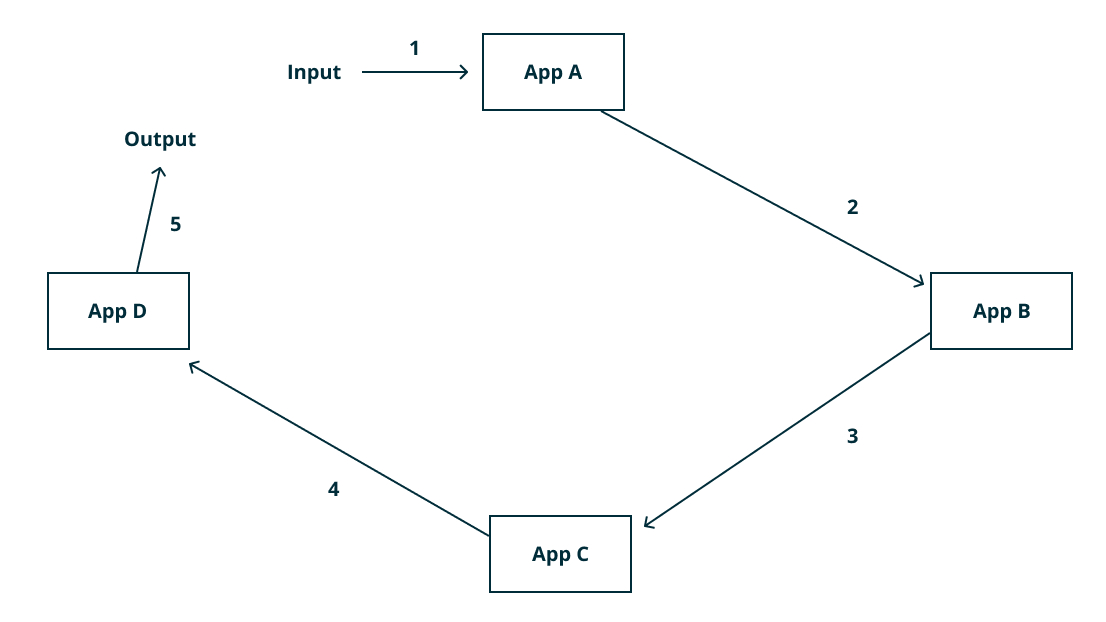
\includegraphics[width=\textwidth, height=0.5\textheight, keepaspectratio]{brokerless.jpeg}
	\caption{Choreographed communication architecture \cite{NoorainPanjwani.2020}}
	\label{img:choreographedCommunication}
\end{figure}

On the other hand, orchestrated architectures need brokers, to which the services connect to.
This eliminates the need for a service discovery, as services are completely decoupled from each other and are more flexible with an asynchronous messaging system (cf. chapter \ref{cha:Theory:async}).
An exemplary flow of communication can be seen in Figure \ref{img:orchestratedCommunication}, where apps/services communicate only over a broker and do not necessarily need a response to a message (e.g \textit{App C}).
The latter case could be a monitoring service, which only collects metrics.
Having a intermediary service, however, always results in a higher latency and higher resource utilization, as compared to direct synchronous communication.
Consequently, broker-based architectures are used over broker-less designs with service discovery in cases, where the benefits such as queueing or broadcasting can be leveraged \cite{Rudrabhatla.2018}\cite{Giro.2019}.

\begin{figure}[h]
	\centering
	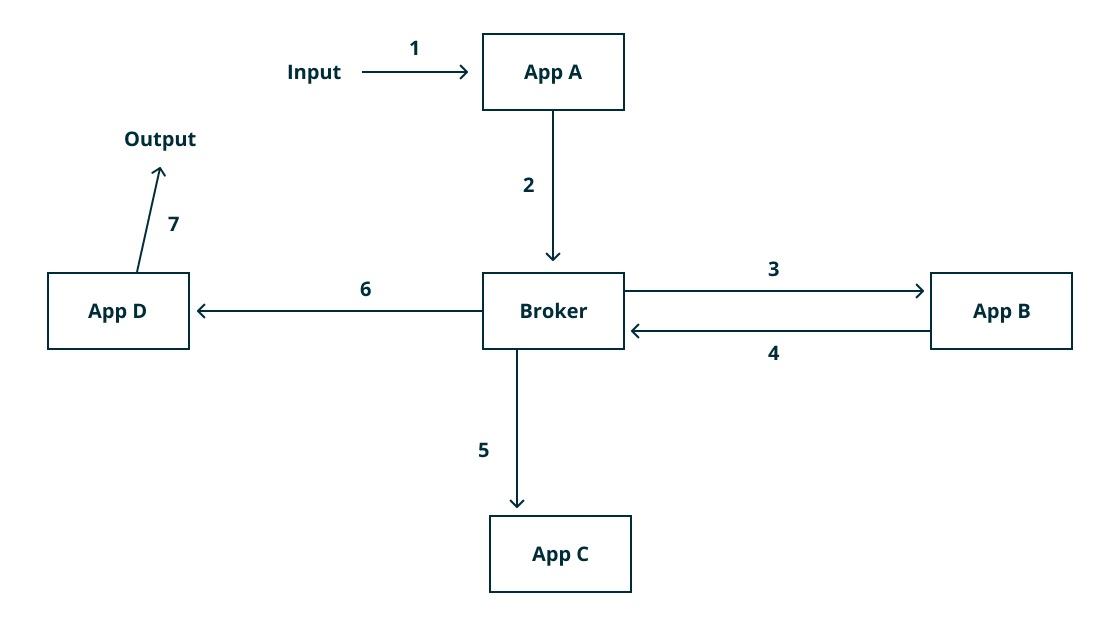
\includegraphics[width=\textwidth, height=0.5\textheight, keepaspectratio]{brokerbased.jpg}
	\caption{Orchestrated communication architecture \cite{NoorainPanjwani.2020}}
	\label{img:orchestratedCommunication}
\end{figure}

\section{Asynchronous messaging}\label{cha:Theory:async}

Asynchronous messaging is used to provide a flexible communication channel between clients.
In such an environment, transferred messages are called events.
As shown in Figure \ref{img:asyncMessagignPrincipal}, a client can either produce or consume events.
To transfer an event, typically a \textit{broker} is needed, which is part of an independent system.
Therefore, the communication flow can be described as follows:
The producer client sends an event to a \textit{broker}, which then routes the event to a consumer client.
Depending on the used \textit{broker}, the available routing mechanisms change.
Routing is an important part of asynchronous messaging \cite[p.~62f.]{Bruce.2019}.

\begin{figure}[h]
	\centering
	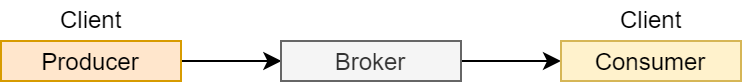
\includegraphics[width=\textwidth, height=0.9\textheight, keepaspectratio]{theorie_async_messaging.png}
	\caption{Asynchronous messaging principal}
	\label{img:asyncMessagignPrincipal}
\end{figure}

Most higher level interaction patterns for asynchronous messaging are based either on the \textit{job queue} or \textit{publish-subscribe} pattern.
The concept of a \textit{job queue} is to distribute work via events to consumers.
To allow this behavior, the \textit{job queue} provides a queue, where producers can send their events to.
Consumers then consume these events, thus emptying the queue.
It is important to note, that not every consumer receives every event.

An example for the \textit{job queue} is shown in Figure \ref{img:asyncJobQueue}.
In this example, an \textit{Order} service creates orders and two \textit{Market} services pickup the events and process them.
As already pointed out, events are not duplicated and hence only one service can consume them \cite[p.~63f.]{Bruce.2019}.

\begin{figure}
	\centering
	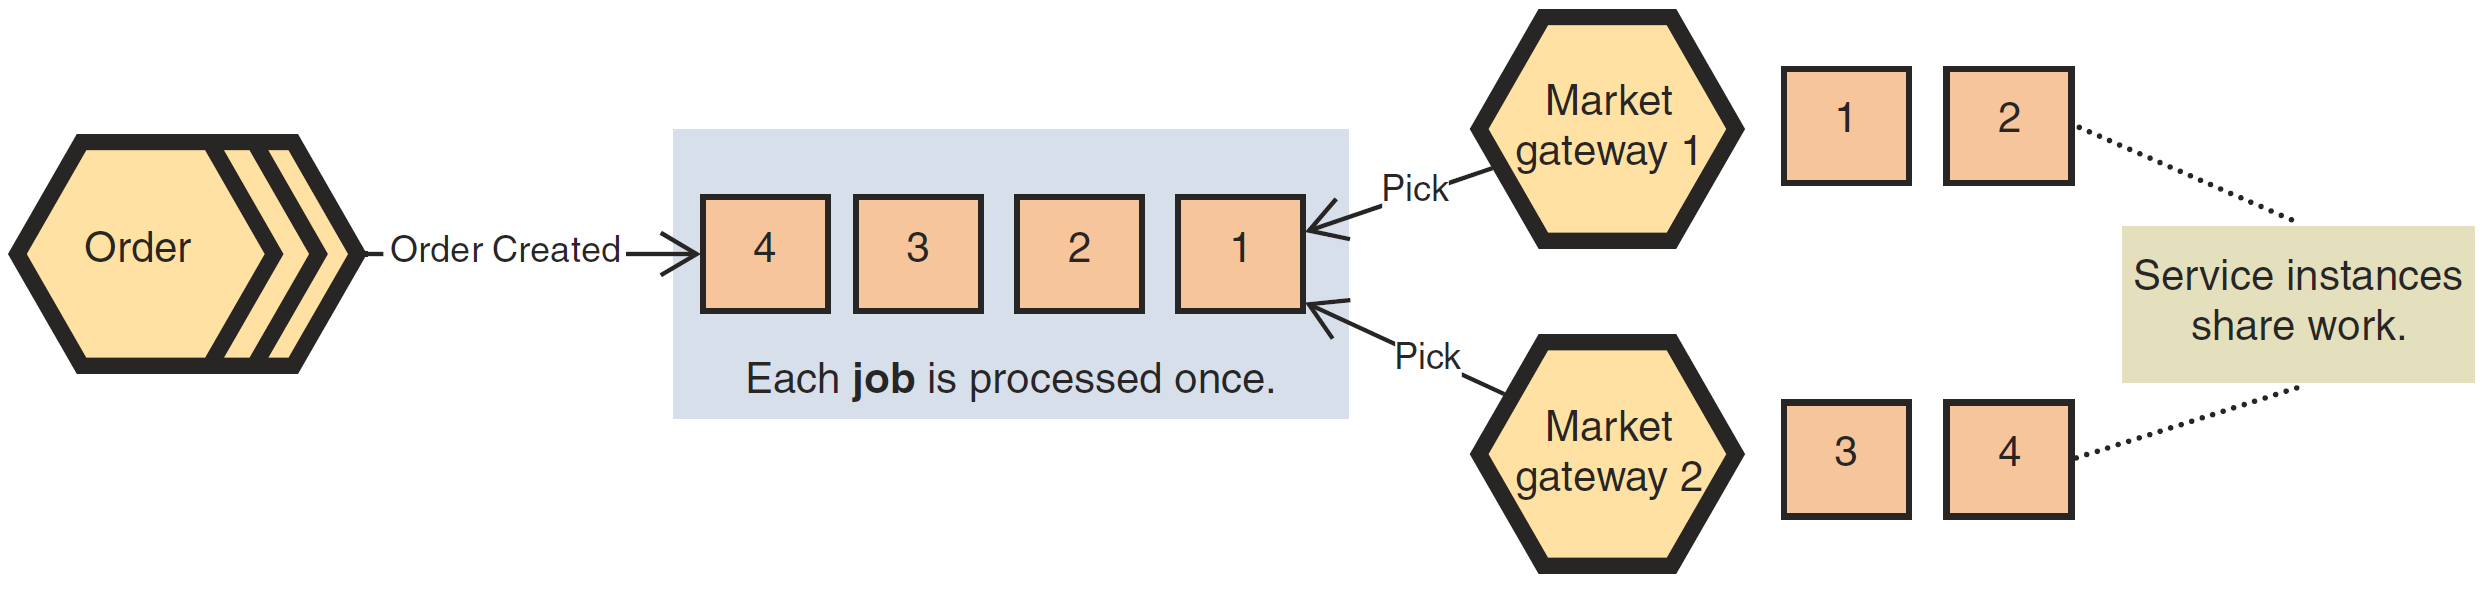
\includegraphics[width=\textwidth, height=0.9\textheight, keepaspectratio]{theorie_async_jobqueue.png}
	\caption{Asynchronous communication pattern job queue example \cite[p.~64]{Bruce.2019}}
	\label{img:asyncJobQueue}
\end{figure}

The second common pattern is the \textit{publish-subscribe} pattern, which is especially important for this work.
The concept of \textit{publish-subscribe} is to inform arbitrary listeners about something.
As the name implies, a client can publish an event which listeners (\textit{subscribers}) receive.
In this case, each event is distributed to each subscriber.
An example for the \textit{publish-subscribe} is shown in Figure \ref{img:asyncPubSub}.
There, a service \textit{Market} publishes the event \textit{oder placed}, which services like \textit{Notify} and \textit{Statistics} subscribe to.
Consequently, all the subscribers receive the event \cite[p.~64f.]{Bruce.2019}.

\begin{figure}
	\centering
	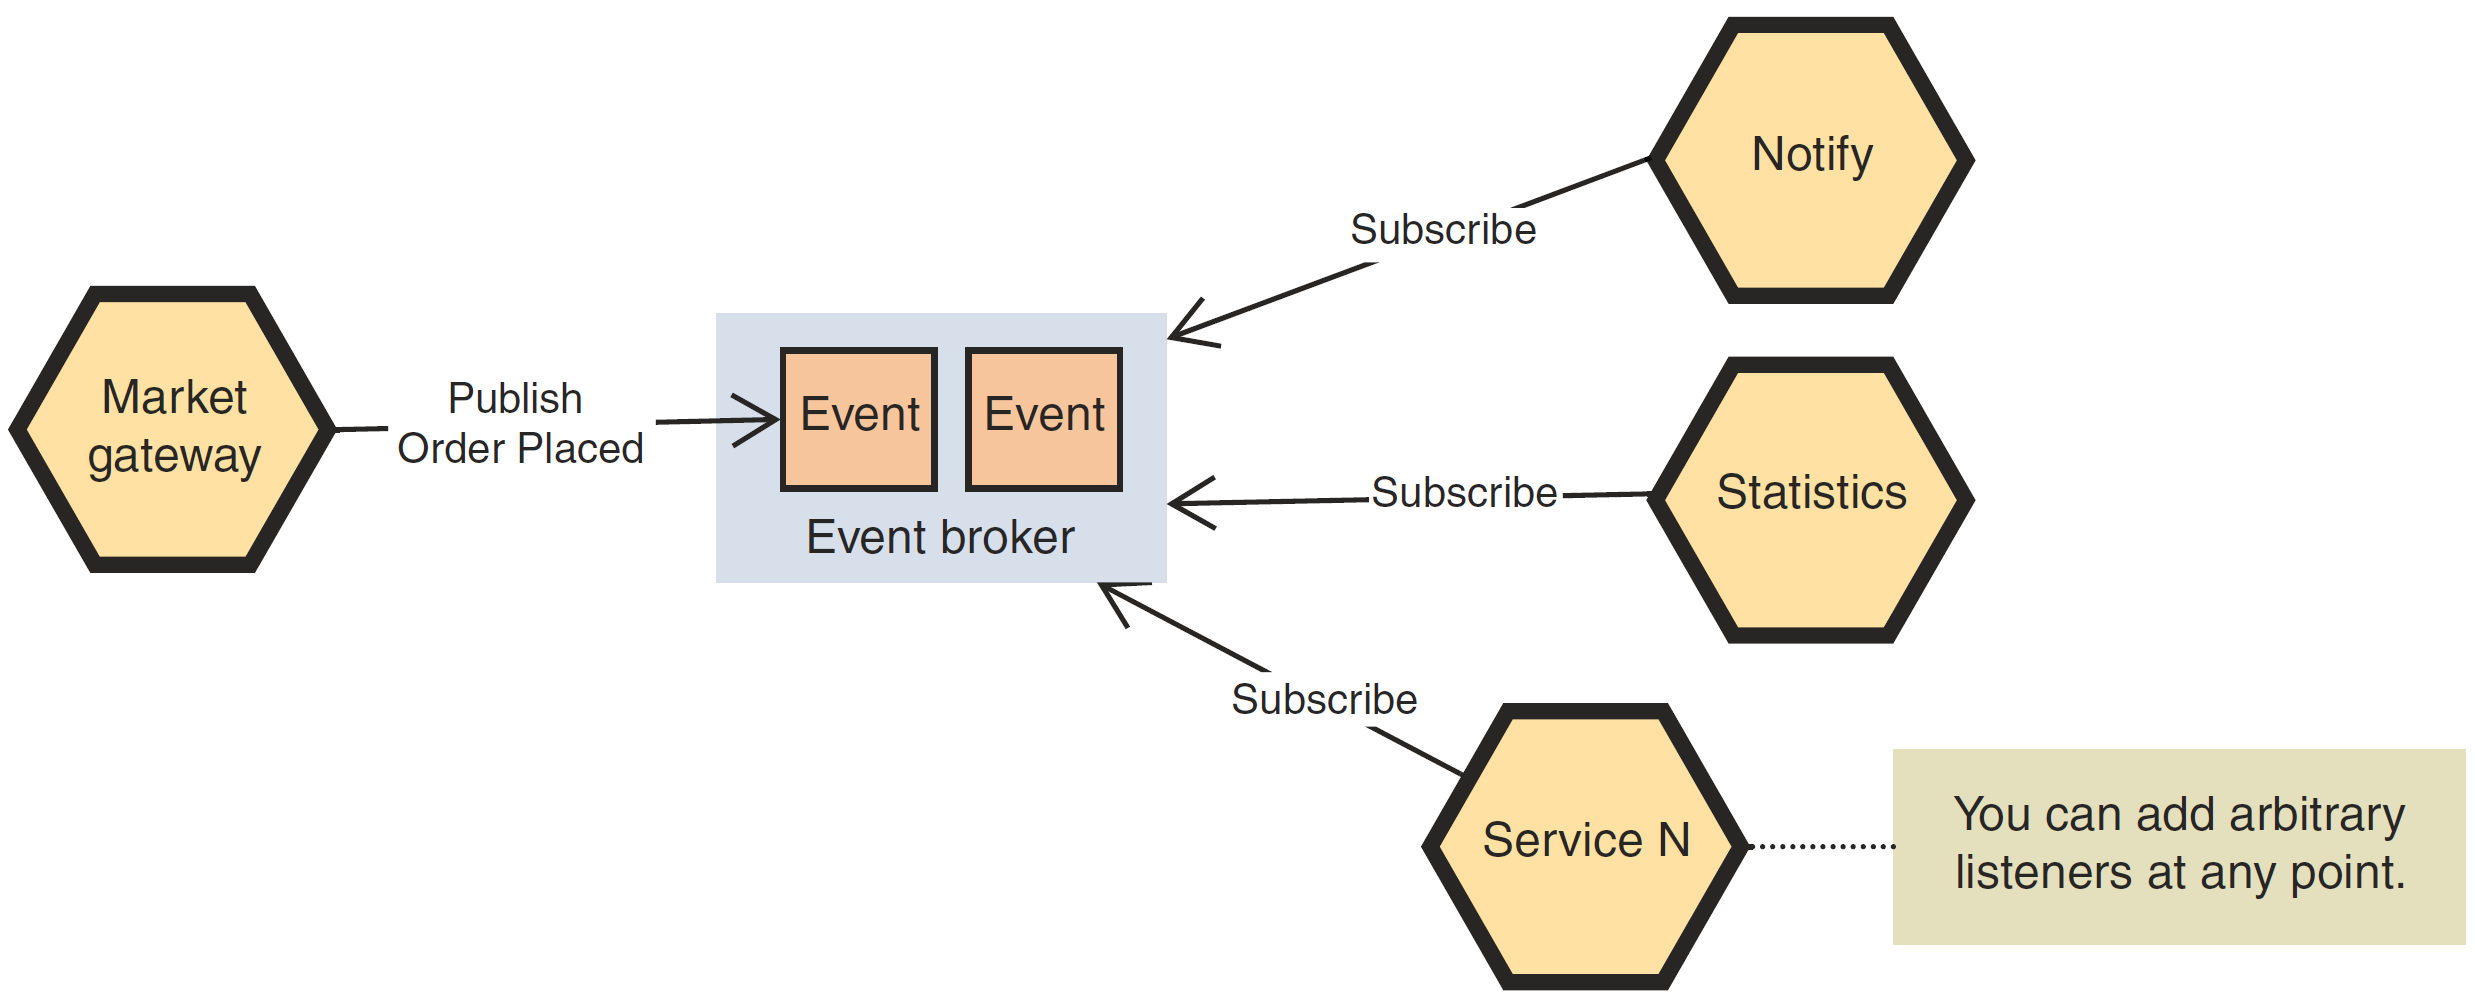
\includegraphics[width=\textwidth, height=0.9\textheight, keepaspectratio]{theorie_async_pubsub.png}
	\caption{Asynchronous communication pattern publish-subscribe example \cite[p.~64]{Bruce.2019}}
	\label{img:asyncPubSub}
\end{figure}

Another important aspect to consider when working with asynchronous messaging are the delivery guarantees.
In the context of the \acf{MQTT} protocol this is called \acf{QoS}.
There are three level of \ac{QoS}, \textit{at-most-once}, \textit{at-least-once} and \textit{exactly-once}.
All levels target the consumer and how events are received in a case of a failure \cite[p.~59f.]{Aziz.08.09.201412.09.2014}\cite{AndrewBanks.2014}.
\begin{itemize}
	\item \textit{at-most-once}: The consumer receives an event once or not at all.
	\item \textit{at-least-once}: The consumer is guaranteed to receive the event, but it could receive the same event more than once.
	\item \textit{exactly-once}: The consumer receives an event exactly once.
\end{itemize}

These \ac{QoS} levels are also applicable to other protocols or technologies.

% Requirement Analysis
%!TEX root = ../dokumentation.tex

\chapter{Requirement Analysis}\label{cha:Requirement}

Some guidelines are needed for the assessment of communication technologies.
The final goal is to create a prototypic \ac{LAN} party management application.
For this purpose, the technologies are compared regarding the functional requirements of the application.
The following section explains the main components of the application.
To further specify the guidelines, personas are selected to represent different views of the stakeholders of such a system with regards to communication.

\section{LAN Party Application}\label{cha:Requirement:lanpartyapplication}
%!TEX root = ../../dokumentation.tex


There are different types and sizes for \ac{LAN} parties.
The purpose of the \ac{LAN} party management application is to manage multiple \ac{LAN} parties over time.
The general idea is that users can create an account, sign up for an upcoming \ac{LAN} party (or event) and participate with their account.
Consequently, the application could contain the following components:

\paragraph{Accounts} are used to identify a user.
Multiple accounts can be grouped to form a team in an event.
This is required for some games.

\paragraph{Events} represent actual \ac{LAN} parties.
They consist of information such as start/end date and a description.
This information could be used for the registration page of an event.
Events could be required to pay a registration fee, which is also part of this component.
Finally, a form of attendee overview could be included.

\paragraph{Scoreboard} is responsible for all matches.
This component therefore contains the following information: participants, played game, used settings and the match result.
It could also be used to manage the game server of the event and to start matches.

\paragraph{Catering} could be part of an event.
Therefore, a list of catering options within the event registration could be used to manage catering.
The result would be an overview of the catering options, chosen by attendees.
This would make it easier to order an actual catering service.

\paragraph{Billing} is an essential part of an event.
A registration is only complete once the registration fee and catering costs have been paid.
A form of billing is therefore required.

\paragraph{Seating plan} option would automate the process of seat selection.
A participant could select a seat in the event room and reserve it in a similar way to reserving a seat in a cinema.

These components/features are used as a general guide for creating the \ac{LAN} party application.
Not every feature is required for every event.
For example, an event might not provide an option for catering.

Lastly, the \ac{LAN} party application architecture will be client-server based, where the client is a web browser.
This modern approach allows for a platform independent use.

\pagebreak

\section{Persona}\label{cha:Requirement:persona}
%!TEX root = ../../dokumentation.tex

There are many combinations of technologies to implement an application based on microservices, but not every combination meets the requirements for such an application.
Technologies must meet the requirements to be useful for an application.
A common practice in web development is to define personas, which have requirements for an application \cite[p. 105]{Castro.2008}.
A persona reflects the interests of a certain group of people.
By defining several personas, several aspects for an application are considered.
Personas have been successfully used in non-Web development projects \cite[P. 105]{Castro.2008} and are used in requirement analysis.

In case of technologies comparison, suitable personas are \textbf{end-user}, \textbf{developer} and \textbf{operator}.
These personas are selected based on the writer's knowledge.
For an end-user, there are many factors that significantly influence the acceptance of the application \cite[p. 245]{Zhou.2008}, but only the performance expectancy can be influenced by communication technologies.
The performance expectancy is important to determine interest of the end-user in the application \cite[p. 244]{Zhou.2008}.
From the end-user's point of view, the application should be performant, so the communication technology must be performant as well.

Developers are primarily interested in whether a communication technology contains all features they need to perform a task.
Sometimes the customer decides which technology to use.
This is the case when a developer is part of a consultant firm and the client has heard of a technology that he wants.
In this case, sometimes a technology is chosen because the customer understands it or is used to it.
When developers have a choice of which technology to use and several technologies contain all the necessary features, they evaluate which technology fits the scenario and meets the performance and scalability requirements the most.
Finally, they consider usability features such as implementation effort and manageability.
Therefore, from a developer's perspective, a communication technology is selected based on performance, scalability, functional requirements and ease of use \cite{ManagingSolutionArchitect.20.05.2020}.

The last persona is the operator.
For this persona, scaling and managing complexity of communication technology is most important.
Features like historization and versioning are a must have and depending on the project, the communication flow must be configurable.
Just like the developer, the operator points out that the customer plays a major role in the choice of communication technology and there is usually little or no choice. Another concern is resilience, which is also a key factor for microservices.
Finally, non-functional requirements such as monitoring and traceability are also important.
Therefore, from an operator perspective, a communication technology is selected based on scalability, resilience and the inclusion of some standard features \cite{EnterpriseArchitectforcloudbasedinfrastructure.20.05.2020}.

After explaining the different needs of personas, Table \ref{tab:requirementsAnalysis} provides an overview of the important factors for each persona. It is used for the technology assessment.
Further information about the interviews for the developer and operator can be found in the appendix at \ref{chp:appendix:interview}.

\begin{table}
	\centering
	\begin{tabular}{ |c|c|c| }
		\hline
		End-User    & Developer   & Operator    \\
		\hline
		Performance & Performance & Scalability \\
		            & Scalability & Resilience  \\
		            & Ease of use &             \\
		\hline
	\end{tabular}
	\caption{Requirement Analysis Overview} \label{tab:requirementsAnalysis}
\end{table}

% Finding Technologies
%!TEX root = ../dokumentation.tex
\chapter{Selection of Technologies for Prototyping}\label{cha:Technologies}

One of the core aspects of a microservice architecture is the communication \cite[p.~60]{Bruce.2019}.
This includes the inter-microservice communication but also the communication beyond the microservice environment to the client itself.
Especially after the deployment, monitoring systems are crucial for operation, in order to collect metrics and observe the system \cite[p.~313]{Bruce.2019}.
With a preceding research, criteria based on the requirements researched in chapter \ref{cha:Requirement} are used to determine, which technology should be tested through prototypes.

\textbf{Researching Technologies}

In order to select technologies and frameworks for development of prototypes for evaluation, research is needed in both aforementioned aspects of a microservice environment, namely communication and monitoring, to find possible technologies.
Although other aspects, such as testing, project build and deployment, and engines are important, these are deliberately left out due to the timely boundaries of this work.
In the following either practical implementations of protocols or complete frameworks for both aspects are presented briefly.

\section{Communication}\label{cha:Technologies:communication}
%!TEX root = ../../dokumentation.tex

Generally speaking, communication can be done synchronously or asynchronously.
In the context of a microservice architecture, asynchronous communication is highly recommended due to its decoupled and non-blocking nature.
Although such an event based communication is favorable in distributed systems, as in microservices, synchronous messaging may also be used, if a specific behavior in another service is needed \cite[p~.34f]{Hofmann.2016}\cite[p.~89]{Newman.2015}.
Consequently, both forms of service communication need to be analyzed separately.

%!TEX root = ../../dokumentation.tex
\textbf{Synchronous Messaging}

For synchronous messaging, the architectural concept of \ac{REST}, the \ac{RPC} framework \textit{gRPC} and lastly the data query language and runtime \textit{GraphQL} are presented.
Although a lot more alternatives are available, the aforementioned options each represent vastly different concepts.
They are selected as they are the most recent and widespread used technology in their category \cite{Mohilo.2019}\cite{Smith.382018}.
Alternatives to \ac{REST} could be \textit{SOAP} (over \ac{HTTP}) for instance.
Likewise, instead of \textit{gRPC}, implementations such as Java RMI, Apache Thrift or even XML-RPC (precursor to \textit{SOAP}) would be viable options as well \cite{Giro.2019}\cite[p.~62f.]{Bruce.2019}.

\subsection{RESTful HTTP}\label{cha:Technologies:communication:rest}

\acf{REST} is an architectural style which focuses on the concept of resources.
Resources shown externally can be completely decoupled from its internal format.
Furthermore, the resources can be encoded in any arbitrary format, such as \ac{HTML}, \ac{XML} or \ac{JSON} and are accessed through resource methods \cite{Restfulapi.net.23.05.2020}.
A further description of the total 6 guiding principles can be seen in Fieldings work \cite{Fielding.15.03.2002}.
In theory \ac{REST} can be used with any underlying protocol, however, in practice \ac{REST} is commonly used together with \ac{HTTP}, hence the name RESTful \ac{HTTP}.
A widely used and recommended model is the Richardson Maturity Model, which describes resource management, the usage of \ac{HTTP} verbs and hypermedia controls \cite{Fowler.2010}.

With the use of \ac{HTTP}, verbs such as \textit{GET}, \textit{POST}, \textit{DELETE}, single endpoints serving multiple purposes are possible, as seen in Table \ref{tab:restExample}.
Furthermore, support of RESTful communication for proxies, caching services and load balancers as well as security measures is available due to the \ac{HTTP} ecosystem.
On the one hand this fact can make \ac{REST} easy to adopt and to ensure interoperability with preexisting architectures.
On the other hand however, this also leads to the necessity of a secure and scalable communication infrastructure (e.g. use of \ac{TLS} for encryption ) as a base \cite[p.~100]{Newman.2015}.

Another benefit, that RESTful communication provides (if implemented according to the Richardson Maturity Model), is the hypermedia control for resources or \enquote{Hypermedia as the enginge of application state} (HATEOAS).
The concept of hypermedia allows clients to perform interactions with the referenced links, embedded in the response.
As requests are only bound to a reference and not beforehand known direct endpoints, clients are abstracted and the implementation can be changed, as long as the semantic of a response does not change.
Consequently, both client and server implementations are decoupled, as the common denominator is the hypermedia control.
Due to the progressive discovery of the \ac{API} that this hypermedia approach entails, the communication may be more verbose, compared to other technologies.

\begin{table}
	\centering
	\begin{tabular}{ |l|l| }
		\hline
		Action               & REST operation               \\
		\hline
		Get news item        & /news/\{id\} \textbf{GET}    \\
		Get (all) news items & /news/ \textbf{GET}          \\
		Delete news item     & /news/\{id\} \textbf{DELETE} \\
		Update news item     & /news/\{id\} \textbf{PUT}    \\
		Create news item     & /news/\{id\} \textbf{POST}   \\
		\hline
	\end{tabular}
	\caption{Exemplary \ac{REST} operations on news item object} \label{tab:restExample}
\end{table}

\subsection{ gRPC}\label{cha:Technologies:communication:grpc}

Developed in 2015 by Google, \textit{gRPC} is an open source \ac{RPC} system, which uses HTTP2 for transport \cite{gRPCAuthors.25.05.2020}.
As it is an \ac{RPC} framework, characteristics, such as tighter coupling, but on the other hand also high performance messaging apply \cite[p.~93f.]{Newman.2015}.
Likewise server and client code can be generated automatically for a variety of targets.
In the case of \textit{gRPC}, as of May 2020, 11 languages are officially supported, namely \textit{C/C++, C\#, Dart, Go, Java, Kotlin, Node.js, Objective-C, PHP, Python, Ruby}.

Unlike \ac{REST}, \textit{gRPC} relies on an \ac{IDL} to define the services, which per default are \textit{protocol buffers} (often abbreviated as \enquote{protobuf})
Apart from using protocol buffers as its \ac{IDL}, \textit{gRPC} can also use it as its message interchange format.
In order for \textit{gRPC} to be able to serialize structured data, each data type may be described in a \textit{*.proto} file, although other similar and popular \acp{IDL}, such as Apache Thrift, as well as \ac{JSON} or \ac{XML} are supported \cite{gRPCAuthors.25.05.2020b}\cite{gRPCAuthors.25.05.2020d}. \\

\begin{lstlisting}[caption=Example of data structure in a \textit{*.proto} file, label=listing:protobufdata]
message Studienarbeit {
string title = 1;
int32 id = 2;
bool passed = 3;
}
\end{lstlisting}

\begin{lstlisting}[caption=Example of service definition in a \textit{*.proto} file, label=listing:protobufservice]
service Greeter {
// Sends a greeting
rpc SayHello (HelloRequest) returns (HelloReply) {}
}

// The request message containing the user's name.
message HelloRequest {
string name = 1;
}

// The response message containing the greetings
message HelloReply {
string message = 1;
}
\end{lstlisting}

An example of such a data object description, using a protocol buffer definition can be seen in Listing \ref{listing:protobufdata}.
With a proto file, according stubs can be generated for target programming languages, by using the protocol buffer compiler \textit{protoc}.
Services to be used can be defined in \textit{gRPC} as well, as seen in Listing \ref{listing:protobufservice} \cite{gRPCAuthors.25.05.2020b}\cite{gRPCAuthors.25.05.2020c}.
The code generated by \textit{protoc} in according target languages can then be used in server and clients as depicted in Figure \ref{img:grpcoverview} \cite{gRPCAuthors.25.05.2020b}.

\begin{figure}[hb]
	\centering
	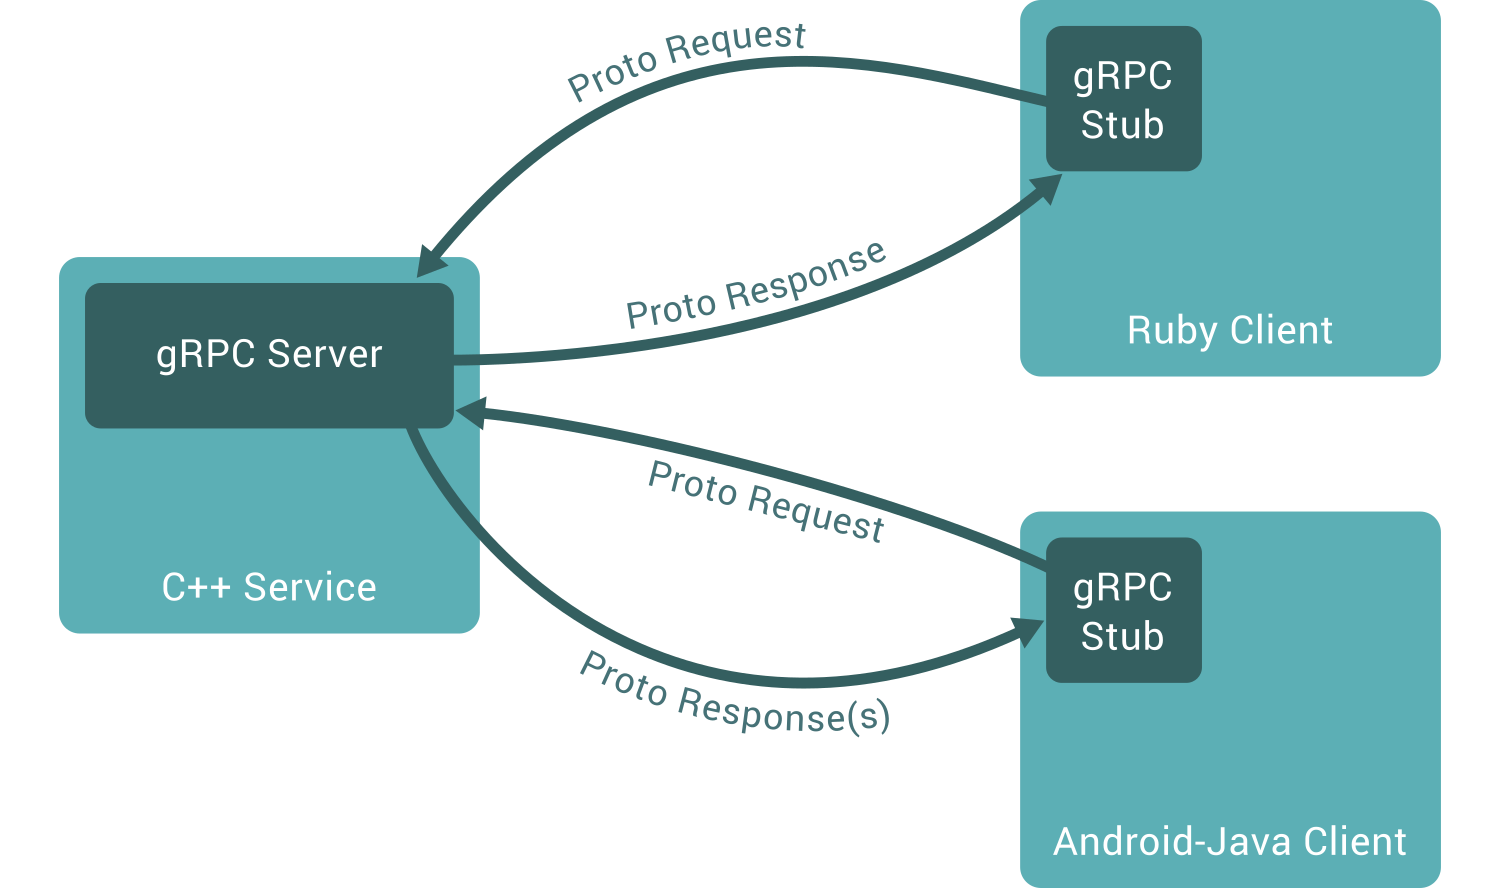
\includegraphics[width=\textwidth, height=0.25\textheight, keepaspectratio]{gRPCoverview.png}
	\caption{gRPC polyglot implementation overview}
	\label{img:grpcoverview}
\end{figure}

A common use case for \textit{gRPC} currently is the inter service communication in microservices, especially, where strict specification and low latency actions need to be executed \cite{Sturgeon.2016}.
The concept of \textit{gRPC} is based around an API contract and strict semantics.
Protocol buffer as a small binary format has a faster serialization (\enquote{de-/marshalling}) and is more efficient, in contrast to the human readable \ac{JSON} used in RESTful \ac{HTTP} applications.
This makes \textit{gRPC} especially useful for network constrained environments and high throughput communication.
As protocol buffer serves as an \ac{IDL}, \textit{gRPC} user have to follow a prescriptive formal specification, as opposed to loose models and implementation levels (e.g. Richardson Maturity Model) \cite{NewtonKing.2019}.

Furthermore, due to the use of HTTP2, \textit{gRPC} supports bi directional streaming, making point-to-point real time communication possible.
Consequently, the need for polling or switching protocols to \textit{WebSocket} for instance can be eliminated.
Other supported forms of streaming are server to client, client to server and unary.

In contrast to \ac{REST}, the usage of \textit{gRPC} in the browser is limited and not supported by default.
Consequently extensions like \textit{gRPC-Web} are needed, which includes an \textit{gRPC} proxy and a JavaScript client for the browser.
Furthermore, \textit{gRPC} messages can not be broadcasted and are not human readable due to protocol buffers being a binary format.
Nonetheless \textit{gRPC} represents a well supported \ac{RPC} communication framework, which is beneficial for efficient inter process communication in distributed client server architectures.
Especially in the context of polyglot microservice environments, the streaming capabilities and low latency of \textit{gRPC} are useful, not only for backend communication but also for applications on (mobile) clients \cite{NewtonKing.2019}\cite{1&1IONOSSE.2020}.

\subsection{GraphQL}\label{cha:Technologies:communication:graphql}

\textit{GraphQL} can be defined as both a data query language as well as a runtime.
The language is used for writing requests for client applications and is close to
\ac{JSON} (as seen in Listing \ref{listing:graphqlquery}).
Contrary to that, the \textit{GraphQL} runtime layer is needed on the server, in order to transform requests into existing logic to fetch data \cite[p.7~f.]{Buna.2016}.
The runtime layer is also responsible for accumulation of different data sources (e.g. composite design pattern seen in Figure \ref{img:compositedesigngraphql})
Although the service is transport agnostic, the most common combination is with \ac{HTTP}.
Furthermore, \textit{GraphQL} has a widespread implementation available similar to \textit{gRPC}, namely \textit{C\# / .NET, Clojure, Elixir, Erlang, Go, Groovy, Java, JavaScript, Julia, Kotlin, Perl, PHP, Python, R, Ruby, Rust, Scala, Swift, OCaml / Reason} \cite{TheGraphQLFoundation.27.05.2020}.

\begin{figure}
	\centering
	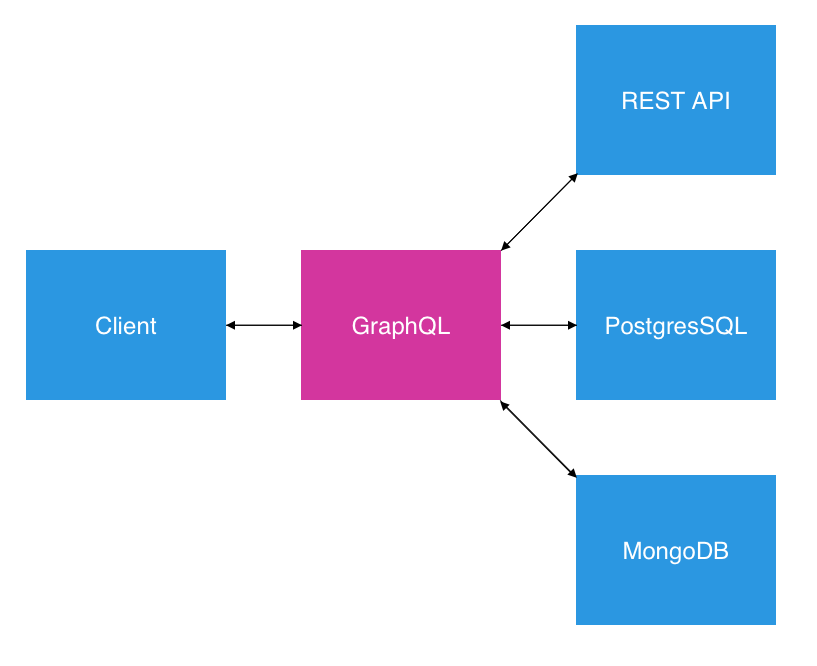
\includegraphics[width=\textwidth, height=0.32\textheight, keepaspectratio]{compositedesigngraphql.png}
	\caption{Composite design pattern in \textit{GraphQL} \cite{Lombard.2018}}
	\label{img:compositedesigngraphql}
\end{figure}

With \textit{GraphQL}, the client specifies the data requirements and only requests the data they need, hence often being referred to as an declarative data fetching language \cite[p.~6f.]{Buna.2016}.
In Listing \ref{listing:graphqlquery} two queries are described, with the according responses seen in Listing \ref{listing:graphqlresponse}.
With the second query, the main characteristics of \textit{GraphQL} are visible \cite[p.~16]{Porcello.2018}:

The data that is served is strongly typed in the \textit{GraphQL} scheme, which makes misuse detection easier \cite[p.~65]{Buna.2016}.
Each data point has a specific type, the scheme \textit{person} has to exist, with predefined field types, such as \textit{filmConnection} as a \textit{PersonFilmsConnection}.
Furthermore \textit{GraphQL} is product centric, which means that it is focused on the clients data needs and the supporting language and runtime.
This also allows for client-specified queries; servers have to provide the capabilities that clients are allowed to consume.
The field \textit{filmConnection} as well as the schemes for the object \textit{films} therefore have to exist.

In cases where the client does not know about the server's type system, the client has to be able to query the scheme with the \textit{GraphQL} language (\textit{Introspection}).
Lastly, every \textit{GraphQL} query can be hierarchical.
Fields can be nested in other fields, as seen with \textit{films} via the \textit{filmConnection}, and the corresponding response is shaped exactly the same \cite[p.~12ff.]{Porcello.2018}\cite[p.~10ff.]{Buna.2016}.

\begin{lstlisting}[caption=Example of GraphQL queries, label=listing:graphqlquery]
// first query
query{
person(personID>5) {
name,
birthYear
}
}
// second query with more fields
query{
person(personID>5) {
name,
birthYear,
filmConnection {
films {
title
}}}
}
\end{lstlisting}

\begin{lstlisting}[caption=Example of GraphQL responses, label=listing:graphqlresponse]
// response to the first query
{
"data": {
"person": {
"name": "Leia Organa",
"birthYear": "19BBY",
}}
}

// response to the second query
{
"data": {
"person": {
"name": "Leia Organa",
"birthYear": "19BBY",
"filmConnection": {
"films": [
{"title":"A New Hope"},
{"title":"The Empire Strikes Back"},
{"title":"The Force Awakens"},
]
}}}
}
\end{lstlisting}

Further exact description about the query language and the scheme as well as the configuration of the runtime are left out in this work, as they are not required for an overview here.

\textit{GraphQL} currently is mostly recommended for Data \acp{API}, especially when the requested data is graph-like.
Similar to \textit{gRPC}, the efficiency through direct querying and low latency, due to the most minimal response size, make \textit{GraphQL} especially useful for applications with a restricted bandwith (e.g. mobile appliances).
RESTful \ac{API} in contrast, may suffer from over- and/or underfetching \cite[p.~3]{Doerrfeld.2018}.

Overfetching occurs when more data is given than actually needed, which may happen especially with large data endpoints with HATEOAS implemented.
On the other hand, when needed data is undercut, the client would have to make multiple requests.
Especially on resource restricted devices, multiple round trips for a single view are inefficient \cite[p.~12f.]{Buna.2016}\cite[p.~24ff.]{Porcello.2018}.
This issue is mitigated in \textit{GraphQL}, as the response is uniform with the request itself.
Moreover, nesting reduces the load on the target device.
In a RESTful API, in order to receive the data of the second request depicted in Listing \ref{listing:graphqlquery}, one would request the \textit{films} of a \textit{person} and receive \textit{filmCollection}, a list of links.
Following that, each link would have to be requested and the field \textit{title} extracted.

\begin{figure}[h]
	\centering
	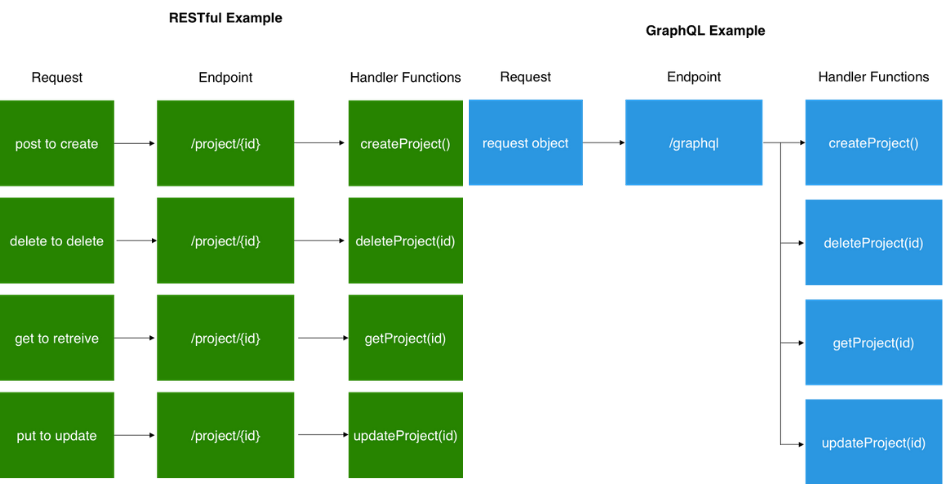
\includegraphics[width=\textwidth, height=0.9\textheight, keepaspectratio]{multiplerestVSgraphql.png}
	\caption{Multiple REST requests vs a single GraphQL request \cite{Lombard.2018}}
	\label{img:restvsgraphqlrequest}
\end{figure}

Furthermore \textit{GraphQL} is easier to scale and maintain due to stronger typing and schema discovery.
Although RESTful \ac{API} implements this with HATEOAS, versioning of endpoints or managing endpoints in general can be cumbersome.
With \textit{gRPC}, flexibility is very limited as it is an \ac{RPC} framework in its nature.
\textit{GraphQL} instead resolves this, by having only one endpoint, with which balancing, orchestration of data sources and version control is possible. (cf. Figure \ref{img:restvsgraphqlrequest})
Consequently, \textit{GraphQL} is the most flexible and scalable when comparing against \textit{gRPC} or a RESTful \ac{HTTP} \ac{API} \cite[p.~29]{Porcello.2018}\cite[p.~11]{Buna.2016}.

Nonetheless, \textit{GraphQL} can be at a disadvantage due to incompatibility with common caching solutions and query complexity.
Each query still needs to be resolved with the target data source, where bottlenecks naturally occur.
This issue especially prevails in situations with a high query depth or query complexity.
Furthermore, rate limiting as typically applied in RESTful \acp{API} are more difficult to apply, because the query depth and complexity weighing can vary a lot \cite{Wieruch.2018}\cite{AltexSoft.2019}.
In most cases, however, \textit{GraphQL} is used as an intermediary, where a \textit{GraphQL} \ac{API} is exposed, but the runtime itself communicates over existing \ac{REST} \acp{API}.
This hybrid proxy variant allows easy adoption and a incremental adoption of \textit{GraphQL} \cite[p.~29]{Porcello.2018}.
\label{cha:Technologies:communication:synchronous}
\clearpage
%!TEX root = ../../dokumentation.tex

\textbf{Asynchronous Messaging}

For asynchronous messaging, the technologies RabbitMQ with its supported protocols, \ac{NATS} and Apache Kafka are presented.
RabbitMQ is used as a representative for all technologies that implement \acf{AMQP}, \acf{MQTT} or \acf{STOMP}.
Apache Kafka is a relatively new technology that has attracted much attention.
It was already introduced in the TechnologyRadar in 2016 \cite{ThoughtWorks.01.06.2020} and a new technique \textit{Event streaming as the source of truth} is becoming more and more popular \cite{ThoughtWorks.01.06.2020b}, which fits perfectly with Apache Kafka.
\ac{NATS} is also quite new, but its main focus is on availability, while RabbitMQ and Apache Kafka focus more on consistency.
Therefore, these three technologies represent a wide range of asynchronous messaging systems.

\subsection{RabbitMQ}\label{cha:Technologies:communication:rabbitmq}

RabbitMQ is an implementation of the \acf{AMQP}.
The protocol follows a Publish-Subscribe pattern.
The communication flow of \ac{AMQP} is shown in Figure \ref{img:rabbitmqamqp}.
It is important to note that multiple publishers can publish to the same exchange entity, one exchange entity can route to multiple queues and multiple consumer can listen at one queue.
The routing of an exchange entity can be configured in four different ways.
To explain the different configurations, it is important to note that each message contains a routing key and can contain n-header information.
Both are used by the exchange entities, but in different ways depending on the configuration.
The following list shows the differences between the configurations in terms of how they route a message to an associated queue \cite{RabbitMQ.2020}\cite[p.~26ff.]{SanjayAiyagarietal.2008}.

\begin{itemize}
	\item Direct: (default) Route a message based on its routing key.
	\item Fanout: Copies the message and sends it to each queue, regardless of the message information.
	\item Topic: Works like Fanout, but also uses the routing key. Queues define regular expressions to determine whether a routing key can be associated with that queue.
	\item Header: Ignores the routing key and uses header information to route a message. This is highly configurable by itself.
\end{itemize}

Exchange entities and queues can be defined in advance or by the publisher and consumer.
If they are defined by the publisher or consumer, the required configuration is provided and sent to RabbitMQ.
When connecting to an exchange or queue its configuration must be provided.
If it doesn't exist, then a new one is created.
If it does exist and the configuration matches the existing one, then a connection is established.
If the provided configuration does not match the configuration of the existing exchange or queue, an error is thrown.
Publisher define exchanges and consumer define queues.
When defining a queue, a binding is required that connects the queue to an exchange entity.
The binding can consist of a routing key (direct exchange), regular expression (topic exchange) or nothing (fanout exchange and header exchange) \cite{RabbitMQ.2020}.

It is important to add that RabbitMQ mostly follows the \ac{AMQP} specification, but small adjustments for usability and functionality extensions were made \cite{RabbitMQ.2020b}.
Also, \ac{AMQP} is not the only standard protocol supported by RabbitMQ.
The protocols \ac{STOMP} and \ac{MQTT} are supported via a plugin as well \cite{RabbitMQ.27.05.2020}.

\begin{figure}
	\centering
	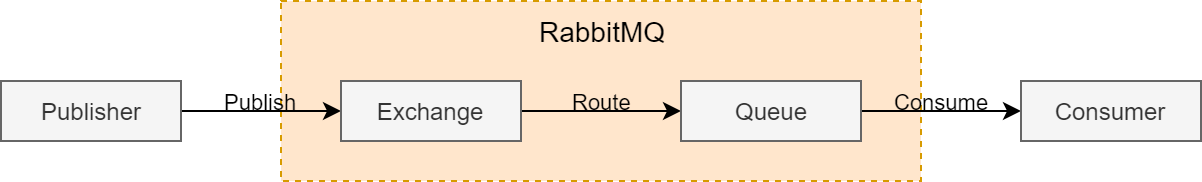
\includegraphics[width=\textwidth, height=0.9\textheight, keepaspectratio]{RabbitMQ_AMQP.png}
	\caption{RabbitMQ communication flow}
	\label{img:rabbitmqamqp}
\end{figure}

\paragraph{STOMP plugin}

As the name suggests, \acf{STOMP} is a simple protocol where messages are sent in frames.
A frame is a text message consisting of a command, an optional header and an optional body.
\ac{STOMP} requires a underlying 2-way streaming network protocol to send frames between client and server.
The communication flow is shown in Figure ~\ref{img:rabbitmqstomp}.
A client can be either a consumer or a publisher.
In both cases, the client only needs to know the connection information of the server for setup.
Unlike \ac{AMQP}, where the client also defines exchanges and queues, \ac{STOMP} requires that the logic is defined in the server.
The clients cannot define the routing behavior of the server, so the server must provide this logic.
To route a message, the server can use anything within it \cite{.25.09.2015}.
The RabbitMQ implementation of \ac{STOMP} has several routing options and each is provided by a separate destination.
To send a message to a specific destination, a \textit{destination string} can be used \cite[p. 191]{Roy.2018}.

\begin{figure}
	\centering
	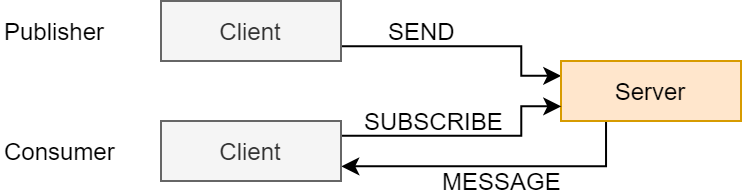
\includegraphics[width=\textwidth, height=0.9\textheight, keepaspectratio]{RabbitMQ_STOMP.png}
	\caption{RabbitMQ communication flow using STOMP}
	\label{img:rabbitmqstomp}
\end{figure}

\paragraph{MQTT plugin}

\ac{MQTT} is located between \ac{STOMP} and \ac{AMQP} from a functionality point of view.
It provides a basic routing like the \ac{AMQP} topic exchange shown in Figure ~\ref{img:rabbitmqmqtt}.
A client can publish a message on a topic (shown in Figure ~\ref{img:rabbitmqmqtt} with topic \textit{cat1/top1} and \textit{cat1/top2}).
A client can also subscribe to topics.
This is shown in Figure \ref{img:rabbitmqmqtt}, where \textit{Subscriber B} subscribes to both topics and therefore receives messages from both topics.
As with \ac{AMQP} topic exchange, the messages are copied and sent to each subscriber \cite[p.~4ff.]{Hillar.2017}\cite{AndrewBanks.2014}.
Finally, each message contains a \acf{QoS} attribute that determines how the message is handled in case of errors \cite{AndrewBanks.2014}.

\begin{figure}
	\centering
	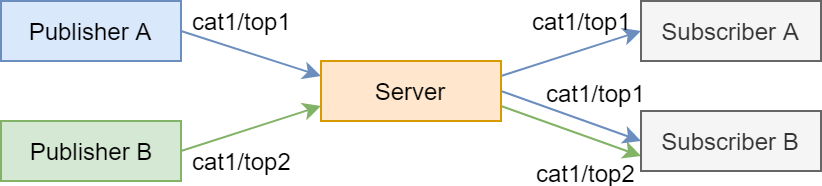
\includegraphics[width=\textwidth, height=0.9\textheight, keepaspectratio]{RabbitMQ_MQTT.png}
	\caption{RabbitMQ communication flow using MQTT}
	\label{img:rabbitmqmqtt}
\end{figure}

\paragraph{Protocol selection}

RabbitMQ can be used in several ways because it supports three protocols.
Consequently, the question remains which protocol to use.
In general, it is advisable to use a protocol that is already supported by an environment.
Another point to consider are the required communication features.
\ac{AMQP} is feature-rich, which can be too complicated for some application environments.
It also has a high latency, which can be a problem for unreliable networking of mobile devices \cite[p. 177]{Roy.2018}.
As described above, \ac{MQTT} has fewer features than \ac{AMQP} and \ac{STOMP} is even more lightweight than \ac{MQTT} \cite[p. 189]{Roy.2018}.
When deciding which protocol to use, it is also helpful to consider other projects.
For example, \ac{MQTT} is often used for \ac{IoT} applications.
This is probably due to the small code footprint or its suitability for low-bandwidth environments \cite[p. 178]{Roy.2018}\cite{AndrewBanks.2014}.
When using \ac{STOMP} the big advantage is that messages are sent in human-readable form (text based), but this is also a disadvantage.
\ac{AMQP} and \ac{MQTT} are binary and therefore more efficient than \ac{STOMP} in transmitting data.
Finally, it is important to mention that the \ac{STOMP} plugin for RabbitMQ adds an overhead, because RabbitMQ uses proxied \ac{AMQP} connections to communicate the translated \ac{STOMP} data \cite[p. 200]{Roy.2018}.

\paragraph{Conclusion}

RabbitMQ is very flexible because it supports several standard protocols, allowing for future technology exchanges.
Which protocol should be used depends on many factors, as described above.
Finally, some important factors that support RabbitMQ for the election, based of the persona needs.

RabbitMQ keeps messages in \ac{RAM} if possible and only when the \ac{RAM} is full, the messages are moved into memory.
To ensure good performance, additional nodes can be added to a running cluster, allowing dynamic scaling.
To ensure availability, nodes can be replicated and the message acknowledgment provides a delivery guarantee.
Another easy to implement feature in RabbitMQ is \textit{multicast}, which can be achieved via a fanout exchange \cite[p.~230ff.]{Dobbelaere.2017}.

\subsection{NATS}\label{cha:Technologies:communication:nats}

The \acf{NATS} is a communication technology that follows the \textit{publish-subscribe} pattern.
Its core objectives are simplicity, performance, and reliability \cite[p.~8]{Quevedo.2018}.
Communication is session-based and a session starts and ends with a connection.
When a session is closed, no data is persisted \cite[p.~3]{Quevedo.2018}.
\ac{NATS} is a non-binary transmission and only provides an \textit{at-most-once} \ac{QoS} when transmitting data \cite[p.~20]{Quevedo.2018}.
There is another popular project called \textit{NATS Streaming}, which adds an abstraction layer over \ac{NATS} and provides an \textit{at-least-once} \ac{QoS} \cite[p.~10f.]{Quevedo.2018}.
It also does not persist or buffer information by default, making it a true \textit{fire and forget} system \cite[p.~8]{Quevedo.2018}.

\ac{NATS} supports the subscription models \textit{fan-out} and \textit{queue subscription}.
Fan-out is the default, and it works like the \ac{AMQP} fanout exchange, but it still uses the subject (or topic in the \ac{AMQP} context).
So, any client that subscribes to a subject will receive all messages in that subject \cite[p.~6]{Quevedo.2018}.
Subjects can be divided into namespaces with a "." (\textit{period}).
A Subscription can be more general by using wildcards, such as "*" (\textit{asterisk}) for partial or token match and ">" (\textit{greater}) for full wildcard \cite[p.~31]{Quevedo.2018}.
Figure \ref{img:natspubsub} shows an example of fan-out communication with multiple clients and namespaces:
\textit{Client C} only receives the message from \textit{Client A}, because it has subscribed the topic \textit{data.test}, whereas \textit{Client D} receives every message published to a subject which starts with the namespace \textit{data}.
Therefore, it receives both messages.

\begin{figure}
	\centering
	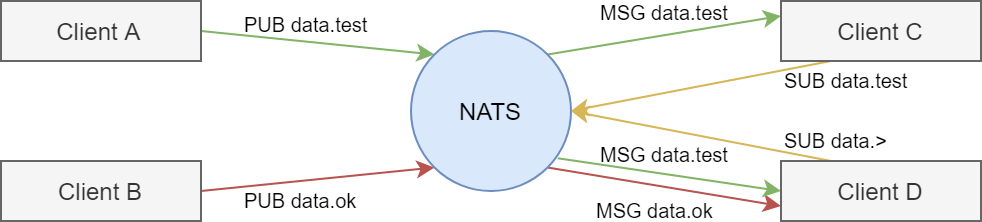
\includegraphics[width=\textwidth, height=0.9\textheight, keepaspectratio]{NATS_Fanout.png}
	\caption{NATS publish subscribe example}
	\label{img:natspubsub}
\end{figure}

The other subscription model \textit{queue subscription} works like \ac{AMQP} \textit{direct exchange}.
When a message is published to a subject, it is distributed to only one subscriber, instead of all.
The two subscription modes can be combined \cite[p.~34ff.]{Quevedo.2018}.
For example, a subject has two clients (\textit{A} and \textit{B}), which are subscribed via a \textit{queue subscription} and one client (\textit{C}) via a \textit{fan-out}.
Then clients \textit{A} and \textit{B} receive messages alternately and \textit{C} receives each message.

A powerful technique of \ac{NATS} is the \textit{request-response} pattern, which enables a completely asynchronous implementation.
An example is shown in Figure \ref{img:natsreqres}, where \textit{Client B} sends a request and \textit{Client A} responds.
This can be archived when \textit{Client B} provides a response subject and its name is passed along with the request.
So, \textit{Client A} knows where to publish the response \cite[p.~38ff.]{Quevedo.2018}.

The Request-Response pattern can be further improved if necessary, by reducing the latency.
To achieve this, \textit{Client A} must be replicated and \textit{Client B} must unsubscribe the response subject, once a message has been retrieved.
It is important that \textit{Client A} and its replicas use the \textit{fan-out} subscription model and the response subject should be unique to avoid collisions.
The result of this approach is that many responses are wasted because only the fastest respond is used.
However, if the main concern is time, this technique allows even faster responses.
Therefore it is called \textit{Lowest Latency Response} \cite[p.~40f.]{Quevedo.2018}.

\begin{figure}
	\centering
	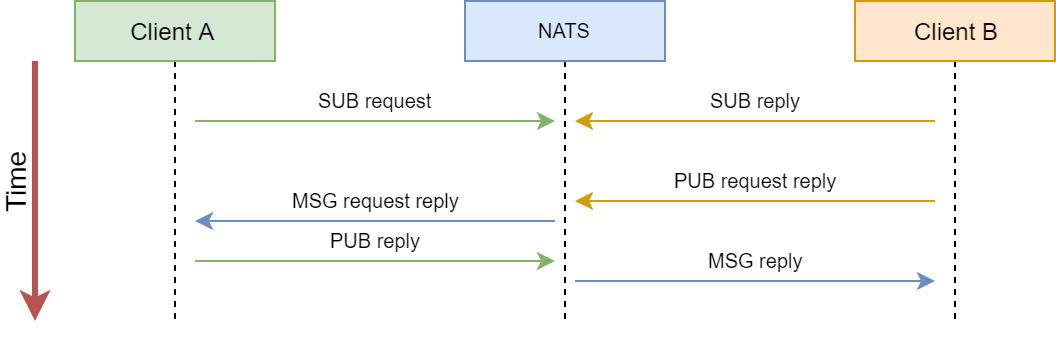
\includegraphics[width=\textwidth, height=0.9\textheight, keepaspectratio]{NATS_request_response.png}
	\caption{NATS request response example}
	\label{img:natsreqres}
\end{figure}

After considering the functionality of \ac{NATS}, the next step is to evaluate it based on the requirements of the personas.
One of the core objectives of \ac{NATS} is performance \cite[p.~8]{Quevedo.2018} and this is illustrated in a benchmark.
For example, in a benchmark comparison between \textit{NATS Streaming} and \textit{Apache Kafka}, \textit{NATS Streaming} was faster in almost every test \cite{TylerTreat.2016}.
It is important to note that \textit{NATS Streaming} uses \ac{NATS} in the core and adds an abstraction layer above it.
This indicates that \ac{NATS} is even faster than shown in the benchmark.
Another important factor is scalability and \ac{NATS} provides a high availability support via a clustering mode that is set up as a full-mesh of servers \cite[p.~8]{Quevedo.2018}.
Another key objective is simplicity \cite[p.~8]{Quevedo.2018}, which is represented by the relatively simple command set.
However, these allow powerful combinations such as mixing of subscription modes \cite[p.~35f.]{Quevedo.2018} and the \textit{Lowest Latency Response} technique \cite[p.~40f.]{Quevedo.2018}.
An important factor to consider is that \ac{NATS} core provides the \textit{at-most-once} \ac{QoS}.
This can be extended to \textit{at-least-once} using the \textit{NATS Streaming} project \cite[p.~10f.]{Quevedo.2018}.
After all, \ac{NATS} tries to stay alive at all costs.
This means that in case of a client connection that accumulates too much data without emptying it, the \ac{NATS} server will disconnect from the client to protect itself \cite[p.~9]{Quevedo.2018}.

\subsection{Apache Kafka}\label{cha:Technologies:communication:kafka}

Apache Kafka (in the following only \textit{Kafka}) is a log-based distributed streaming platform and offers high availability, storage and linear scale-out \cite[p.~14]{Stopford.2018}.
For fault tolerance and linear scale-out, the data is distributed across many machines \cite[p.~17f.]{Stopford.2018}.
\textit{Kafka} is suitable for a variety of applications, but before describing them, it is important to explain how \textit{Kafka} works.

Like the other asynchronous communication technologies, \textit{Kafka} follows the \textit{publish-subscribe} pattern.
This means that a client can publish a message to a topic, and a subscribed consumer receives the message.
In \textit{Kafka}, a message is treated like a log, which means that it is immutable and added to a message log.
The topics are divided into partitions \cite[p.~30]{Kumar.2017}, and each partition has its own message log \cite[p.~33]{Kumar.2017}.
To determine which message is routed to which partition, the message key is used \cite[p.~41]{Kumar.2017}.
To ensure high availability, topic partitions are replicated, where one partition is the leading partition and the others are the following partitions.
If the leader fails, a new leader is selected from the followers \cite[p.~33]{Kumar.2017}.

Partitions and their replicas are distributed among several brokers \cite[p.~17]{Stopford.2018}, and a broker can only have one or two partitions of the same topic.
A \textit{Kafka} cluster consists of several nodes, which in turn have several brokers \cite[p.~27]{Kumar.2017}.
This combination allows \textit{Kafka} to scale particularly well, so that it is no problem to have 100 nodes or even more \cite[p.~20]{Stopford.2018}.

The next important part of \textit{Kafka} is \textit{Zookeeper}.
It is responsible for several tasks, and without it \textit{Kafka} would not work.
For example, \textit{Zookeeper} takes care of the broker states, because broker do not persist their state \cite[p.~27]{Kumar.2017}\cite[p.~37f.]{Kumar.2017}.
\textit{Zookeeper} also knows the distributed locations of the partition leaders and followers \cite[p.~34]{Kumar.2017}.

A client who sends messages to a topic is called a producer, and a client who receives messages is called a consumer.
Each consumer belongs to a consumer group, and a consumer group can consist of several consumers \cite[p.~36f.]{Kumar.2017}.
Within a consumer group, only one consumer can be assigned to a topic partition.
This limits the degree of parallelism in a single consumer group \cite[p.~30f]{Kumar.2017}.
To publish or subscribe to a topic, the publishers or consumer needs to know which topic partition is relevant for them.
This means that a message is published or consumed directly from a topic partition, rather than from a topic.
Publishing or consuming a message is only possible from a topic partition leader \cite[p.~33]{Kumar.2017}\cite[p.~36]{Kumar.2017}.

All the parts described are combined in the Figure \ref{img:kafkacomflow}, where an example communication is shown.
The actual message transmission is only a small part, and a lot of work is done beside it.
In addition, the described communication flow shows the standard behavior, which can be changed.

Before any communication can take place, \textit{Zookeeper} must collect information about the locations of the topic partition (\textit{1}).
This information is then distributed to the producers and consumers (\textit{2}).
Now the producer knows the destination for the message and sends it to the lead partition \textit{A} (\textit{3}).
Partition \textit{A} stores the message and then informs \textit{Zookeeper} and the publisher about the successful writing (\textit{4}).
\textit{Zookeeper} then informs the consumer about a new message that is available (\textit{5}).
Now consumer \textit{A} can read the new message (\textit{6}) and updates its state at \textit{Zookeeper} (\textit{7}).

\begin{figure}
	\centering
	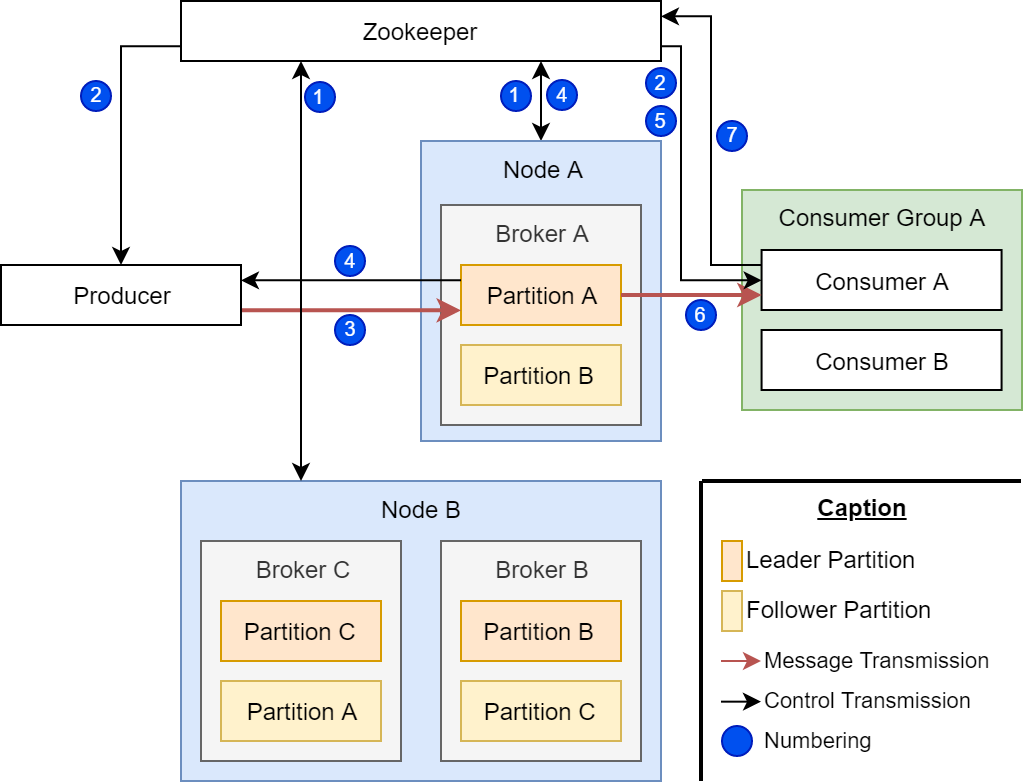
\includegraphics[width=\textwidth, height=0.9\textheight, keepaspectratio]{kafka_communication_flow.png}
	\caption{Kafka communication flow}
	\label{img:kafkacomflow}
\end{figure}

The last important part to complete \textit{Kafka}'s explanation is the message log within a partition.
Publishing a message to a message log within a partition involves several steps.
The process is shown in Figure \ref{img:kafkapubmsg}.
After a leading partition receives a message, it calculates the message offset, which is the identifier of a message within a partition.
The message is then appended to the message log, but not committed \cite[p.~18]{Stopford.2018}.
In addition, the message is sent to all its partition followers.
Each follower partition replies with an acknowledgment, and once everyone has responded, the message is committed to the message log.
The final step is to inform the producer that the message has been accepted and the \textit{Zookeeper} that a new message is available \cite[p.~36]{Kumar.2017}.

\begin{figure}
	\centering
	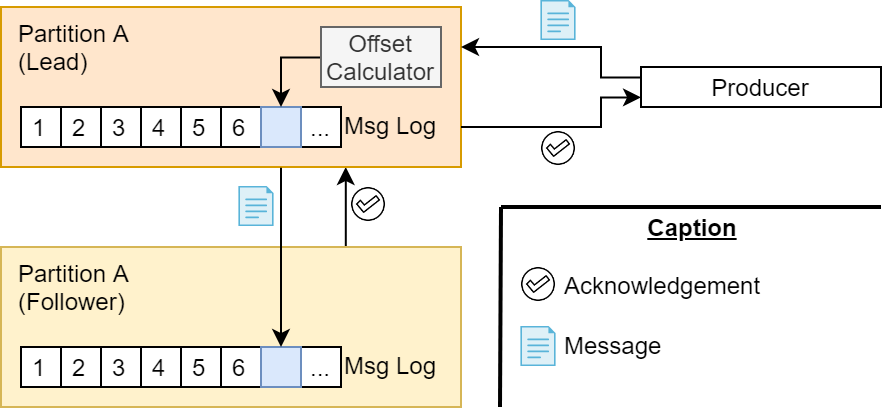
\includegraphics[width=\textwidth, height=0.9\textheight, keepaspectratio]{kafka_publish_message.png}
	\caption{Kafka publish message example}
	\label{img:kafkapubmsg}
\end{figure}

After explaining \textit{Kafka} and the concepts on which it is based, the open question arises as to what \textit{Kafka} is good for.
\textit{Kafka} can be used as a messaging system, which has already been described in the above communication example.
This includes the two traditional models of \textit{queue} and \textit{publish-subscribe}.
Queuing is realized by having multiple consumers within a consumer group.
Messages from a topic can only be consumed by one consumer within a consumer group.
There is an important side effect that the maximum number of consumers within a group is equal to the number of topic partitions.
On the other hand, \textit{publish-subscribe} is handled in such a way that several consumer groups can listen to the same topic.
In this way, each consumer group receives a published message.

Another specialty of \textit{Kafka} is its storage system.
Published messages are stored on disk, and Kafka’s disk structure enables good performance even when terabytes of data are stored.
The messages can be re-consumed as needed, making \textit{Kafka} a distributed file system for special purposes, designed for high performance, low-latency and replication.
The last feature of \textit{Kafka} is its ability to process data streams.
\textit{Kafka} provides a \textit{Streams API} that can consume and process messages from one topic and publish them to another topic.
This is very flexible because it uses the same interfaces as the actual producers and consumers \cite{ApacheKafka.01.06.2020}.

This concludes the general structure and major characteristics of \textit{Kafka}, but there are more features that are explained in \cite{Stopford.2018} and \cite{Kumar.2017}.
For example, an important feature that should be considered here is the message order guarantee.
\textit{Kafka}s default settings only guarantee message order within a partition.
It can be extended to guarantee the order within a topic or even globally, but this is associated with a high-performance overhead \cite[p.~30]{Kumar.2017}.
Another important fact is that \textit{Event Sourcing} architecture fits perfectly with \textit{Kafka}, since it can store messages like a database and replay the message log at any time.
Even if \textit{Kafka} is complex under the hood, it is still quite easy to use.
There are some quality of live features, such as not having to worry about queue depth and that slow consuming messages do not affect performance, which makes \textit{Kafka} easier the use.
\textit{Kafka}'s unique architecture allows for high speed reading of messaged.
Messages can be sent directly from storage because they are immutable logs.
As described at the beginning, \textit{Kafka} scales with virtually no limitations.
Finally, it offers countermeasures for denial of service attacks with a feature called \textit{quotas} \cite[p.~18ff.]{Stopford.2018}.
\label{cha:Technologies:communication:asynchronous}

\pagebreak
\section{Monitoring}\label{cha:Technologies:monitoring}
%!TEX root = ../../dokumentation.tex

In distributed systems, monitoring can be significantly more difficult than monitoring a monolithic architecture.
Metrics, like latency, traffic, errors and saturation as defined by the \textit{Google Site Reliability Engineering}, are essential from the DevOps perspective, but also for other business units.
In terms of microservices, monitoring makes necessary thresholds visible for scaling and can help to decide whether applications need to be broken down further and scaled individually.
Furthermore showing long term trends, retrospective analysis (e.g. for debugging) and especially alerting are core features of a monitoring system \cite{Ewaschuk.02.12.2019}.

\begin{figure}
	\centering
	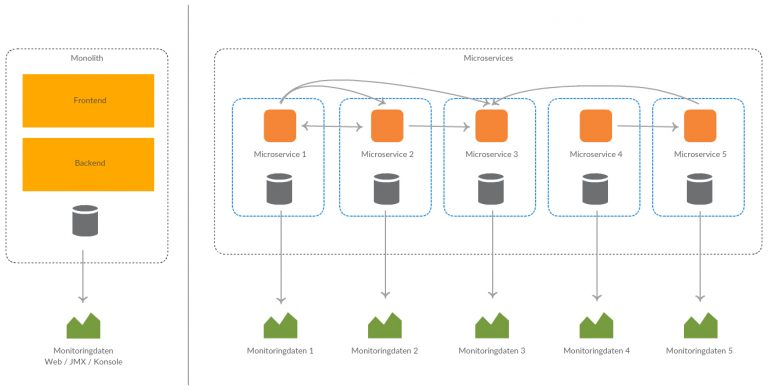
\includegraphics[width=\textwidth, height=0.9\textheight, keepaspectratio]{monitoringMonolithicComparison.jpg}
	\caption{Monolithic monitoring is easier to gather than with microservices~\cite{Fichtner.2016}}
	\label{img:monitoringMonolithicComparison}
\end{figure}

As opposed to a monolith, each microservice generates its own set of monitoring data, these have to be gathered and combined for a meaningful representation.
In order to pinpoint potential issues, metrics and logs from each service (depicted in Figure \ref{img:monitoringMonolithicComparison}) have to be centralized.
This aggregation can be done by either pushing or pulling.
Monitoring frameworks such as \textit{Prometheus} are pulling metrics from services, which have to implement an endpoint and serve data.
The implementation of a metrics endpoint is often called \textit{exporter}.
Time-series databases which do not primarily are built for monitoring (e.g. \textit{InfluxDB}, \textit{Graphite}) have to rely on data collection daemons, which are pushing data to the databases.
Popular daemons for example is the system-metric focused \textit{collectd} or the plugin-driven\textit{Telegraf}, with which a variety of services are supported at once \cite{Fichtner.2016}\cite{Richardson.20.05.2020}\cite{Ewaschuk.02.12.2019}.

In general, aforementioned metric collection daemons are inter-compatible.
Although \textit{Telegraf} would work best with \textit{InfluxDB}\footnote{Referring to the \textit{TICK} stack for centralized alerting and monitoring from the same company \textit{influxdata}: \textit{Telegraf}, \textit{InfluxDB}, \textit{Chronograf} (visualization) and \textit{Kapacitor} (data streaming engine)}, the metric output can be directed to other time-series databases like \textit{Graphite} and even replace the data ingest for \textit{Prometheus} \cite{Loschwitz.2018}.

For this work, the focus is on the time series database itself, as the data aggregation can be interchanged and are mostly compatible to one another.
Furthermore external visualizations such as \textit{Grafana} or \textit{Chronograf} are left out.

\begin{figure}
	\centering
	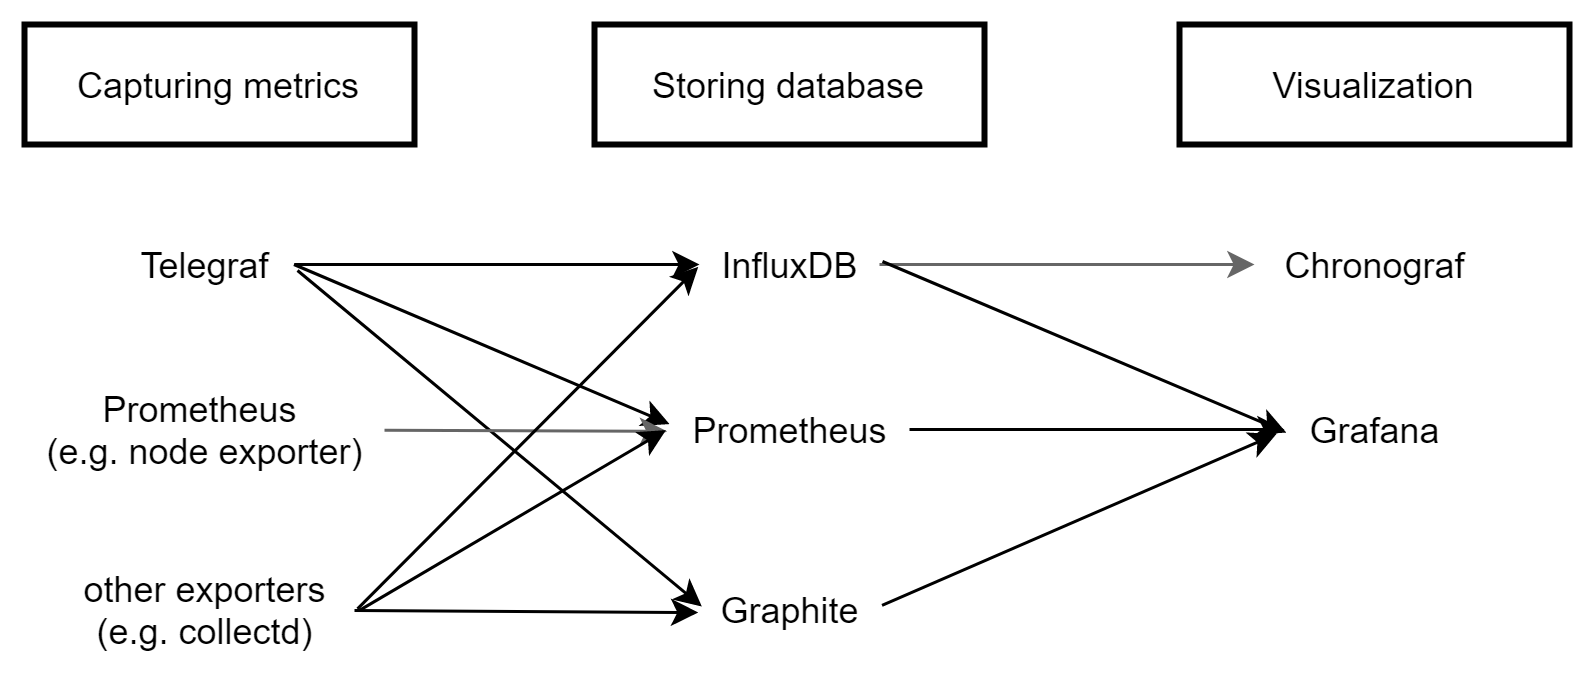
\includegraphics[width=\textwidth, height=0.9\textheight, keepaspectratio]{overviewmonitoring.png}
	\caption{Overview of an selection of popular monitoring technologies}
	\label{img:overviewmonitoring}
\end{figure}

\subsection{Graphite}

As a real-time graphing system based on Python, \textit{Graphite} is able to store numeric time-series data and render graphs.
In order to do so it consists of three main components, as shown in Figure \ref{img:overviewgraphite}, namely the daemon \textit{carbon}, the database library \textit{whisper} and the \textit{graphite webapp} for visualization \cite{Davis.08.05.2020b}.
Unlike \textit{Prometheus} for instance, it relies on inbound metric submissions and does not collect data actively.
Consequently, applications or nodes to be monitored have to be equipped with collection tools, which either communicate over TCP or UDP as plain text, using Python's \textit{pickle} protocol or \ac{AMQP} \cite[p.~49]{Dixon.2017}\cite{Davis.08.05.2020c}.

In most cases, however, tools already support the format, as seen in Listing \ref{listing:graphitemessage}, and handle metrics export and communication with \textit{Graphite}'s \textit{carbon-cache}.
An extensive list of currently supported collectors as well as further compatible tools, which should be used in conjunction, can be found in the \textit{Graphite} documentation \cite{Davis.08.05.2020d}.

\begin{lstlisting}[caption=Graphite Message Format, label=listing:graphitemessage]
metric_path value timestamp
\end{lstlisting}

\begin{lstlisting}[caption=Graphite's dot oriented naming scheme, label=listing:graphitemetricnaming]
api_server_http_requests_total.post.500.tracks.sample1 
\end{lstlisting}

The logical component \textit{carbon} as shown in Figure \ref{img:overviewgraphite} consists of a relay, an aggregator and the actual required \textit{carbon-cache}.
The latter represents the core to accept metrics over aforementioned protocols.
A \textit{Graphite} message (if not bundled using Python's \textit{pickle}) contains the metric namespace to be populated (\textit{metric\_path}), the \textit{value} and a timestamp, as seen in Listing \ref{listing:graphitemessage} \cite{Davis.08.05.2020c}.
\textit{Graphite}'s metrics naming is dot oriented and implies hierarchy.
In Listing \ref{listing:graphitemetricnaming} an exemplary metric name is given for HTTP POST requests with the \textit{response code 500} landing on the \textit{/tracks} endpoint.

\begin{figure}
	\centering
	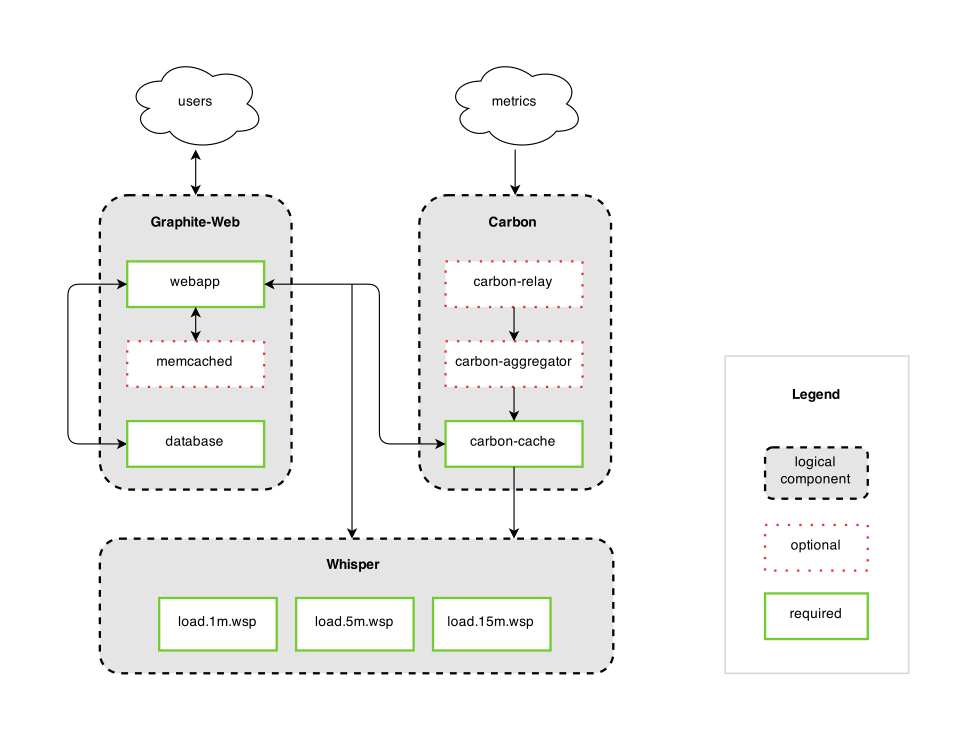
\includegraphics[width=\textwidth, height=0.8\textheight, keepaspectratio]{graphiteoverview.png}
	\caption{Overview of Graphite's architecture \cite{Davis.08.05.2020}}
	\label{img:overviewgraphite}
\end{figure}

The relay is needed for scaling the \textit{carbon-cache} processes, which can be on different servers.
However, in practice typical load balancers such as \textit{HAProxy} are used in front of the logical component \textit{carbon} as a whole to split metrics and thus scaling \textit{Graphite} \cite{Dubiel.29.05.2020}.
In order to reduce load, an aggregator can be used to buffer metrics before saving them using \textit{whisper}, which is a fixed sized database file format for datapoints \cite[p.~52]{Dixon.2017}.
Each \textit{*.wsp} file in\textit{whisper} needs corresponding scheme definitions for retention policies and precision settings.
These settings can be used to duplicate metrics with a lower precision to save space, while removing the original after its retention duration \cite[p.~55]{Dixon.2017}.
Lastly \textit{graphite-web} can be used to visualize data in real-time from the \textit{whisper} storage and \textit{carbon-cache} simultaneously.


The performance of \textit{Graphite} is generally bound to the \ac{I/O} performance of the system.
Usually this is mitigated by increasing the disk array, placing aggregators and load balance between them.
Although this way of vertical scaling is supported well, horizontal scaling can be cumbersome, as one has to decide between redundancy (replication factor) or high performance by utilizing consistent hashing across all instances \cite[p.~57ff.]{Dixon.2017}.
Possible currently used and common alternatives to avoid the scaling problem, are replacing the underlying \textit{whisper} storage engine (e.g. with \textit{InfluxDB}) or replacing the relay with alternative implementations (e.g. \textit{carbon-relay-ng} written in Go) to achieve higher performance.

\subsection{InfluxDB}

\textit{InfluxDB} is a time series database and provides an SQL-like query language (\textit{InfluxQL}) for data interaction, unlike \textit{Graphite}.
The company \textit{influxdata}, provides an open-source version (\textit{InfluxDB OSS}) and a commercial version (\textit{InfluxDB Enterprise}).
Although \textit{InfluxDB} has a higher performance than \textit{Graphite}, as shown in an extensive technical paper, including benchmarks, and thus would be a very good database for monitoring usages, it can not be taken into consideration due to missing features \cite{influxdata.2019}.
The main reason is the missing clustering option for the database.
In the open-source variant, high availability is not guaranteed and horizontal scalability through sharding is not available.
Especially when deploying a high demanding application, such as a large management application, operating \textit{InfluxDB} on a single node seems to be insufficient \cite{influxdata.2020}.
Consequently, no overview will be given here as non open-source and especially paid features are not in the scope of research, leaving \textit{InfluxDB OSS} not suitable.

\subsection{Prometheus}

Similar to \textit{Graphite}, \textit{Prometheus} is primarily used for system monitoring and includes a time-series database and a monitoring system.
Currently \textit{Prometheus} is part of the \textit{Cloud Native Computing Foundation} and open source.
Besides storing and retrieving metrics, it also includes an alerting system and a web \ac{UI}.
Moreover, \textit{Prometheus} has a broad support of clients, by using exporters on the client side.
Unlike other monitoring solutions which depend on passive listeners and clients pushing metrics to the service, \textit{Prometheus} mainly relies on pulling \cite{Berman.2018}\cite{PrometheusAuthors.30.05.2020}.

\begin{figure}
	\centering
	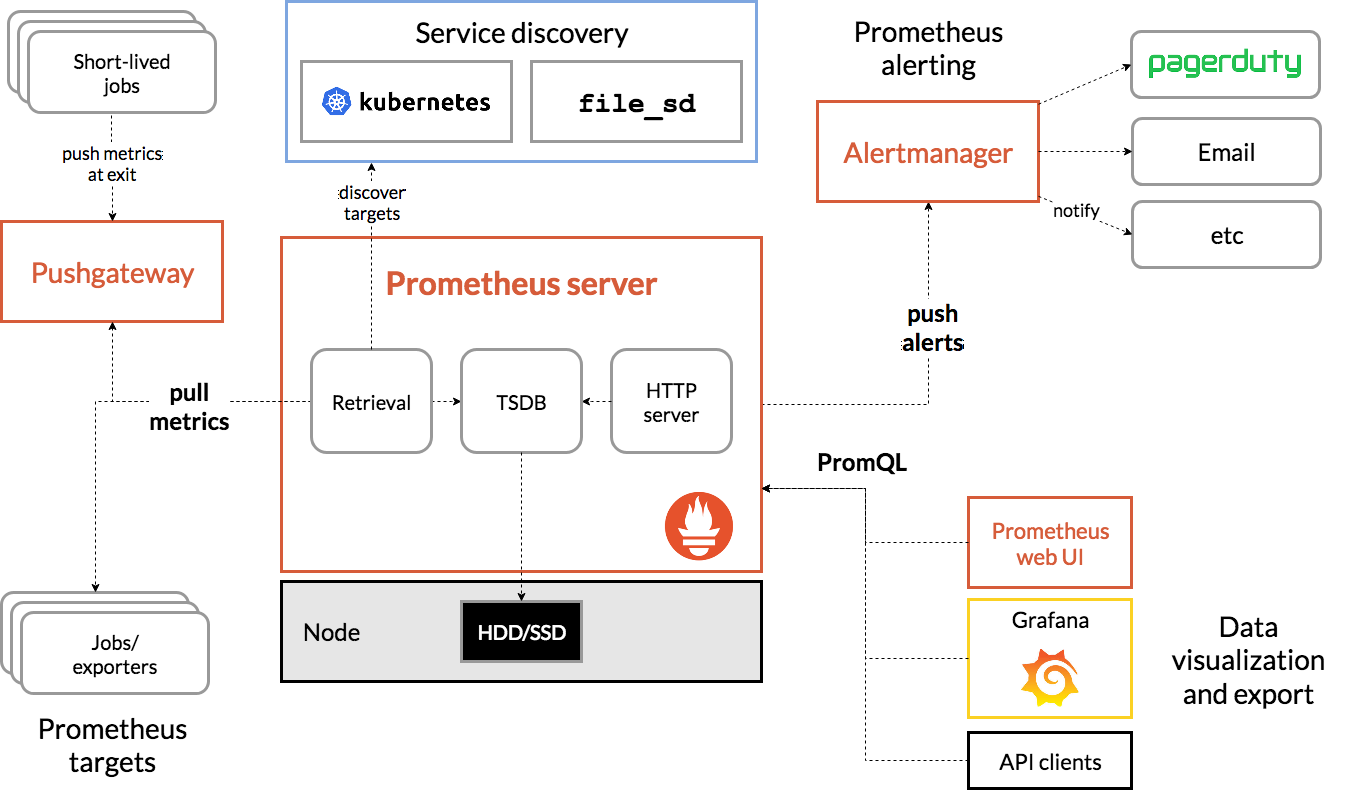
\includegraphics[width=\textwidth, height=0.8\textheight, keepaspectratio]{prometheusoverview.png}
	\caption{Overview of Prometheus' architecture \cite{PrometheusAuthors.30.05.2020}}
	\label{img:prometheusoverview}
\end{figure}

As seen in Figure \ref{img:prometheusoverview} metrics are pulled from \textit{Prometheus} target, which expose their metric on a \ac{HTTP} endpoint.
Consequently, \textit{Prometheus} handles data scraping itself and stores it in an internal \ac{TSDB}.
Although the concept of pulling is favored, \textit{Prometheus} is compatible with existing \enquote{pushing} clients as well, by utilizing the intermediary \textit{Pushgateway}, which stores and aggregates data.
For the active pulling, the endpoints can either be static, or be discovered by utilizing external service registries.
Apart from collecting and storing metrics, events and alerts can be configured in the \textit{Alertmanager} for sending notifications.
Lastly, external visualizations and clients can communicate with \textit{Prometheus} using its own \textit{Prometheus Query Language (PromQL)} \cite{PrometheusAuthors.30.05.2020}.

Similarly to \textit{Graphite}'s \textit{whisper}, time series are stored locally and are grouped into blocks.
With \textit{Prometheus}, incoming samples are kept in memory first and are secured with a write-ahead-log, before being persisted and grouped into two hour blocks.
Like \textit{Graphite}, retention policies and compression options are available for the \ac{TSDB} format.
This approach however, can limit the scalability and durability of the system, as the local storage is bound to the performance of a single node, especially with the concept of node autonomy found in \textit{Prometheus}.
Possible solutions are to replace the \ac{TSDB}, against remote storage systems, to which \textit{Prometheus} communicates with protocol buffers over \ac{HTTP} \cite{PrometheusAuthors.30.05.2020b}.

\textit{Prometheus} is generally known for the variety of exporters available for \acp{API}, messaging systems, hardware related metric systems and also databases. (see \cite{PrometheusAuthors.30.05.2020c} for an extensive list)
Instead of converting existing metrics to the \textit{Prometheus} exposition format, using aforementioned exporters, client libraries are available as well, with which metrics of an application are defined and exposed.

Similar to the \textit{Graphite} message format (see Listing \ref{listing:graphitemessage}), one can also write raw messages, which include the metric name, value and timestamp \cite{PrometheusAuthors.30.05.2020d}.
However, the data model of \textit{Prometheus} allows more complex metadata models by including \enquote{labels}, i.e. key values pairs.
Depicted in Listing \ref{listing:prometheusmessage} is an exemplary metric of the number of HTTP POST requests with the \textit{response code 500} to the \textit{/tracks} endpoint.
This explicit multidimensionality allows greater flexibility compared to the implicit dimension encoding found in \textit{Graphite}, which makes progressive changes in naming difficult to maintain (compare Listings \ref{listing:graphitemetricnaming} and \ref{listing:prometheusmessage}) \cite{Berman.2018}\cite{PrometheusAuthors.30.05.2020e}.

\begin{lstlisting}[caption=Prometheus exposition format with example, label=listing:prometheusmessage]
// syntax: metric_name{label_name = label_value, ...} value [timestamp]

api_server_http_requests_total{method="POST",handler="/tracks",status="500"} 34
\end{lstlisting}

With the aforementioned concept of write ahead logs for instance, reliability is one of the core principles.
The autonomy of each \textit{Prometheus} instance allows access to metrics, even under failure conditions.
However, just like \textit{Graphite}, scaling may be difficult.
A common approach is splitting up the metrics to be monitored and the \textit{Prometheus} instance bound to it, which would value the autonomy aspect.
Alternatively \textit{Prometheus} can scale horizontally by sharding , which means that a subset of metrics are scraped by slaves (partitioning) and are then federated by the master \cite{Brazil.2015}\cite{Berman.2018}.

\pagebreak
\section{Selection}\label{cha:Technologies:selection}
%!TEX root = ../../dokumentation.tex

\subsection{Synchronous Communication}\label{cha:Technologies:selection:synchronous}

When comparing the three presented synchronous messaging technology, \textit{gRPC} is the most performant, thus fulfilling the requirements of the user and developer (cf. chapter \ref{cha:Requirement:persona}) the most.
Its binary format (\textit{protocol buffer}), as opposed to \ac{JSON} used in \textit{GraphQL} and \ac{REST}, is more efficient and beneficial in cases with low network throughput or limited resources.
However, due to missing official support of \textit{gRPC-Web} and due to its incomplete implementation, communication between the web-based frontend and any backend can only be achieved with \ac{REST} and \textit{GraphQL}.
Consequently \textit{gRPC} could only be used for backend communication in this use case.

\begin{table}[h!]
	\begin{tabularx}{\linewidth}{ |l| X | X | X | }
		\hline
		&
		RESTful HTTP & GraphQL                                                                   & gRPC                                                                                                                                                                      \\
		\hline
		Protocols   & Synchronous communication over HTTP only                                  & Synchronous or asynchronous in multiple protocols (e.g. HTTP, AMQP, MQTT)           & Synchronous communication in HTTP2 (although asynchronous implementation available) \\
		Design      & HTTP (verbs, links, status codes)                                         & Based on exchanging messages                                                        & Messages (e.g. protocol buffer payload)                                             \\
		Standards   & Multiple standards available (e.g. Richardson Maturity Model, OpenAPI)    & Schema definition as a standard (\ac{IDL}) Strongly typed                           & Service definition in protocol buffer file for instance (strongly typed as well)    \\
		Payload     & \ac{JSON} for instance                                                    & \ac{JSON}                                                                           & Serialized in binary(default is protocol buffer)                                    \\
		Integration & Nearly every client                                                       & Specific implementation in clients needed (wrapping in \ac{HTTP} endpoint possible) & Specific and tightly coupled implementation for clients needed                      \\
		Endpoint    & Endpoints need to be known, hypermedia possible with HATEOAS for instance & Single endpoint, self-describing scheme                                             & Concrete methods have to exist on both sides                                        \\
		Scaling     & Easy to scale due to stateless nature                                     & Scaling only limited by data source access bottlenecks                              & Scaling similar to REST as HTTP2 is used                                            \\
		\hline
	\end{tabularx}
	\caption{Overview synchronous communication \cite{Rocha.2019}}
	\label{tab:overviewSynchronousCommunication}
\end{table}

Regarding the scalability of the application, all three technologies excel and provide high performance endpoint access.
Load balancing is possible with all three of them with \textit{gRPC} being the most advanced due to HTTP2.
Another aspect is the ease of use and the maintainability of the protocol.
Contrary to the loosely specified \ac{REST}, both \textit{GraphQL} and \textit{gRPC} provide strong typing by enforcing schema/service definitions.
This makes validation and error handling easier for both sides.
Although having specified schemes, \textit{GraphQL} is the most flexible compared to \textit{gRPC}, due to its nature being an \ac{RPC} framework.
With \textit{gRPC}, concrete methods and response actions have to be implemented, while also having to update the client when changes occur.
Consequently \textit{gRPC} introduces tight coupling between services.
On the other side is \textit{GraphQL} with a flexible requests and an introspective, self-describing single endpoint.
\ac{REST}, however fares worse in comparison, as there are no endpoint specifications per default and issues such as over- and underfetching may occur.

Tight coupling in a microservice may not be necessarily bad practice, as it can bring benefits in a tightly coupled network of services, such as low latency and high efficiency found in \textit{gRPC} \cite{Esposito.2019}.
However, in the case of the exemplary use case in this work, loose coupling is better with a modular approach for adding new components to the application.
This renders \textit{gRPC} with its coupling by design disadvantageous, compared to \textit{GraphQL} and \ac{REST}.

In conclusion, \textit{gRPC} represents a highly efficient but tightly coupled system, whereas \textit{GraphQL} allows flexible and maintainable data queries and RESTful \ac{HTTP} being a widespread used, but less standardized and possibly less efficient way of messaging.
An overview is given in the Table \ref{tab:overviewSynchronousCommunication}.

Albeit \textit{gRPC} being developed out of the need for performant and low latency microservice communication, the support for the component in the architecture with the most intensive synchronous communication, namely frontend to backend is incomplete \cite{gRPCAuthors.01.06.2020}.
Regarding inter-service communication, in which \textit{gRPC} dominates and \textit{GraphQL} on the other hand is unsuited, broker-based communication may be preferable.
This is due to the fact that the different components are emitting events affecting multiple other components, instead of just having to trigger a function with a point to point connection like with \ac{RPC} (e.g. ending a match affects both the component \textit{Scoreboard} and \textit{Events}, cf. chapter \ref{cha:Requirement:lanpartyapplication}).
All things considered \ac{REST} and \textit{GraphQL} are prototyped and evaluated in this work, although \textit{gRPC} might be an option to be considered in the future for this use case, with coming web application support.


\pagebreak

\subsection{Asynchronous Communication}\label{cha:Technologies:selection:asynchronous}

If one compares the three asynchronous messaging technologies presented, \ac{NATS} is the most performant and thus meets the requirements of the personas (cf. chapter \ref{cha:Requirement:persona}) the most.
In a benchmark comparison between \ac{NATS} Streaming and \textit{Apache Kafka}, \ac{NATS} Streaming was faster in almost all tests \cite{TylerTreat.2016}.
However, this performance has its price, as \ac{NATS} does not persist messages.
Therefore, they are lost if no consumer listens for them.
On the other hand, \textit{RabbitMQ} provides mechanisms to route messages that are not read, and \textit{Apache Kafka} stores the messages, which eliminates the problem altogether.

\begin{table}[h!]
	\begin{tabularx}{\linewidth}{ |l| X | X | X | }
		\hline                                                                                            &   
		RabbitMQ                                                                                          &   
		NATS                                                                                              &   
		Apache Kafka                                                                                        \\
																
		\hline
		Protocol                                                                                          &   
		\ac{AMQP}, \ac{MQTT} and \ac{STOMP}                                                               &   
		NATS                                                                                              &   
		Kafka                                                                                               \\
																
		Communication                                                                                     &   
		Publish-Subscribe and Queue                                                                       &   
		Publish-Subscribe, Queue and Request-Response                                                     &   
		Publish-Subscribe, Queue and Streaming                                                              \\
																
		Payload                                                                                           &   
		\ac{AMQP} and \ac{MQTT} is binary and \ac{STOMP} is plain text                                    &   
		plain text                                                                                        &   
		developer can choose \cite{RobinMoffatt.2018}                                                          \\
																
		Quality of Service                                                                                &   
		\textit{at-most-once}, \textit{at-least-once} and \textit{exactly once} \cite{PaoloPatierno.2018} &   
		\textit{at-most-once} and \textit{at-least-once} (if \textit{NATS Streaming} is used)             &   
		\textit{at-most-once} and \textit{at-least-once} \cite{AjmalKaruthakantakath.2016}                  \\
		Queue Storage                                                                                     &   
		Limited                                                                                           &   
		None                                                                                              &   
		Permanent                                                                                           \\
		\hline
	\end{tabularx}
	\caption{Overview asynchronous communication}
	\label{tab:overviewAsynchronousCommunication}
\end{table}

All three technologies provide a sophisticated scaling solution that enables high availability.
Another aspect is usability, which is difficult to measure because it is subjective.
To simplify this, only the complexity of available commands is used as a measurement.
This leaves \textit{RabbitMQ} with the \ac{AMQP} protocol behind \ac{NATS} and \textit{Apache Kafka}, because connecting to a queue or exchange requires extensive configuration.
On the other hand, \ac{NATS} and \textit{Apache Kafka} strive for a simple interface \cite[p.~8]{Quevedo.2018} \cite[p.~18]{Stopford.2018}.
However, \textit{RabbitMQ} also supports \ac{MQTT} and \ac{STOMP} via plugin, which simplifies the necessary configuration.
It is important to note that simplicity does not mean that only simple structures are possible.
As far as resilience is concerned, each technology has its own clues to ensure it.
Interesting features include \textit{Apache Kafka} \textit{quotas} \cite[p.~21]{Stopford.2018} and the fact that \ac{NATS} will break connections if the consumer becomes too slow \cite[p.~9]{Quevedo.2018}.

From the persona perspective, \ac{NATS} and \textit{Apache Kafka} would be selected, but it is also important that the technologies fits the exemplary use case in this work.
The components of the use case were presented in the requirement analysis (cf. chapter \ref{cha:Requirement:lanpartyapplication}).
The communication between them is the important aspect when choosing an asynchronous messaging technology.
There is no obvious communication scenario in which extreme performance would be required.
Even if, for example, the \textit{billing} component takes 10 seconds to communicate with the \textit{event} component, no problem should occur.
Therefore, the components should work independently of each other, and eventual consistency is acceptable if the communication provides the \ac{QoS} \textit{at-least-once}.

In summary, \textit{RabbitMQ} and \textit{Apache Kafka} meet the requirements "out of the box", and if \textit{NATS Streaming} is used instead of \ac{NATS}, all three technologies can be used.
However, selection is required, so \ac{NATS} is not selected because it does not provide the required functionality out of the box.

\subsection{Monitoring}\label{cha:Technologies:selection:monitoring}

Regarding the monitoring of a microservice environment, important aspects are the performance, ease of use and the resilience of the system. (cf. chapter \ref{cha:Requirement:persona})
Another aspect is the scalability, which, due to the limited options of horizontal scaling for both options, is neglected here.
Both technologies do allow scaling via sharding and/or federation mechanisms, which, however, creates disadvantageous coupling.

The ease of use overall is greater with \textit{Prometheus}  than with \textit{Graphite} , due to the larger compatibility with various client services.
It should be noted however, that the initial setup and metric pushing is easier with \textit{Graphite}  due to the raw communication protocols.
Especially with simpler services to be monitored, or short running jobs, avoiding heavy \ac{HTTP} handling is favorable.
Moreover the push based metric collection in \textit{Graphite}, allows it to be flexible, as it does not need a service discovery, which \textit{Prometheus}  needs to avoid static endpoint links \cite{Erez.2019}.


However, the relatively more complicated manual integration of instrumentation libraries in order to export metrics in the \textit{Prometheus}  message format, can be neglected, as third-party exporters are available.
This extensibility with metric exporters, which allow very easy integration of services, make \textit{Prometheus}  more favorable in a possibly highly diverse and polyglot microservice environment.
Although this does cause additional dependencies and requires \textit{Prometheus}  to
run inside the same network, due to the pull strategy unlike \textit{Graphite} , the higher performance of \textit{Prometheus}  is overweighing.
\textit{Graphite} 's ingestion process for example be overwhelmed, when sending a lot of datapoints, rendering the pushing concept disadvantageous \cite{Erez.2019}\cite{Frazier.2019}.

\begin{table}[h!]
	\begin{tabularx}{\linewidth}{ | l | X | X | }
		\hline
		Feature                 & Prometheus                                                           & Graphite                                                       \\
		\hline
		Metric input            & Server scrapes/pulls metrics from clients                            & Metrics are pushed to Graphite                                 \\
		Communication protocols & HTTP-based endpoint                                                  & TCP, UDP, AMQP                                                 \\
		Metric discovery        & Service discovery with Kubernetes for instance                       & no client discovery                                            \\
		Metric naming scheme    & Naming system using labels (key-value)                               & Hierarchical dot notation                                      \\
		Data operations         & Prometheus Query Language \textit{PromQL}                            & Graphite Functions                                             \\
		Client support          & More complicated initial setup, but many exporters available already & Simple metric export, but fewer support. Custom scripts needed \\
		\hline
	\end{tabularx}
	\caption{Comparison monitoring Graphite and Prometheus \cite{Erez.2019}\cite{Frazier.2019}\cite{Berman.2018}}
	\label{tab:comparisonmonitoring}
\end{table}

When comparing the resilience, \textit{Graphite} 's push strategy forces clients having to update the endpoint, when changes occur to the monitoring system, making a failover less flexible.
While \textit{Graphite}  does support external storage clusters and thus provide redundancy, autonomous \textit{Prometheus}  instances do not support any type of redundancy when a cluster fails, as any metric requests have to pass through \textit{Prometheus} , regardless of the data source.
On the other hand, \textit{Prometheus}  provides inbuilt monitoring of containers, essential to microservices.
Moreover, \textit{Prometheus}  is able to monitor uptime through the metric scraping/pulling process \cite{Berman.2018}\cite{Erez.2019}.

To conclude, \textit{Prometheus}  has various benefits such as an ecosystem of exporters and client instrumentation, which reduces the more complex nature of \textit{Prometheus} .
On the contrary, \textit{Graphite}  has a simpler format and communication structure, partly due to the incorporated push strategy.
A brief comparison overview can also be found in Table \ref{tab:comparisonmonitoring}.
For the microservice architecture to be built in this work, \textit{Prometheus}  is chosen, due to the integration capabilities with other services through modular exporters, the service discovery capabilities and the higher performance.
The aforementioned traits are essential in an application like a \ac{LAN} party management tool, where high user interaction with a diverse backend occurs.
Additionally there are other topics of \textit{Prometheus} , which are not covered here, but are important for this specific use case, namely event tracking, alarming and the extensive query language \textit{PromQL}.

A prototypic implementation for both technologies, however, is left out in the following, as monitoring is highly variable regarding the architecture.
Each monitoring solution might work better, depending on the metrics to be monitored and the used technologies.
As each technology has different metric reporting solutions for delivering or exporting data to corresponding monitoring technologies, an evaluation whether \textit{Graphite}  or \textit{Prometheus}  would work best, can only be done after selecting other components in a microservice environment.
The communication technology and services for the exemplary application however, still have to be evaluated with prototypes.
Consequently the choice for \textit{Prometheus}  made here should be considered with caution, and may not be applicable to every microservice environment.


% PoC Implementation 
%!TEX root = ../dokumentation.tex

\chapter{Proof-of-concept Implementation}\label{cha:Implementation}

\section{Synchronous Communication RESTful HTTP and GraphQL}\label{cha:Implementation:sync}
%!TEX root = ../../dokumentation.tex

For both RESTful \ac{HTTP} and GraphQL, the same initial setup will be used for prototyping.
Naturally, \textit{node.js} serves as the base engine for interacting with the specific implementation (yellow in Figure \ref{img:prototypesynccomm}), whether it is to provide multiple RESTful \ac{API} endpoints or a single GraphQl endpoint.
For the mockup data to be served over either of the communication technologies, \textit{MongoDB} was chosen together with \textit{Mongoose} as a database connector/driver, due to preexisting experience with said tools.

The exemplary use case is an \ac{API}, which provides information about chefs and dishes. The latter are referenced with a \textit{chefsID} to the chef the dish belongs to.
It should be possible for the client to enter new chefs and dishes, modify, update and delete them, as well as to get an overview of all elements stored in the database (brown in Figure \ref{img:prototypesynccomm}).

\begin{figure}[h]
	\centering
	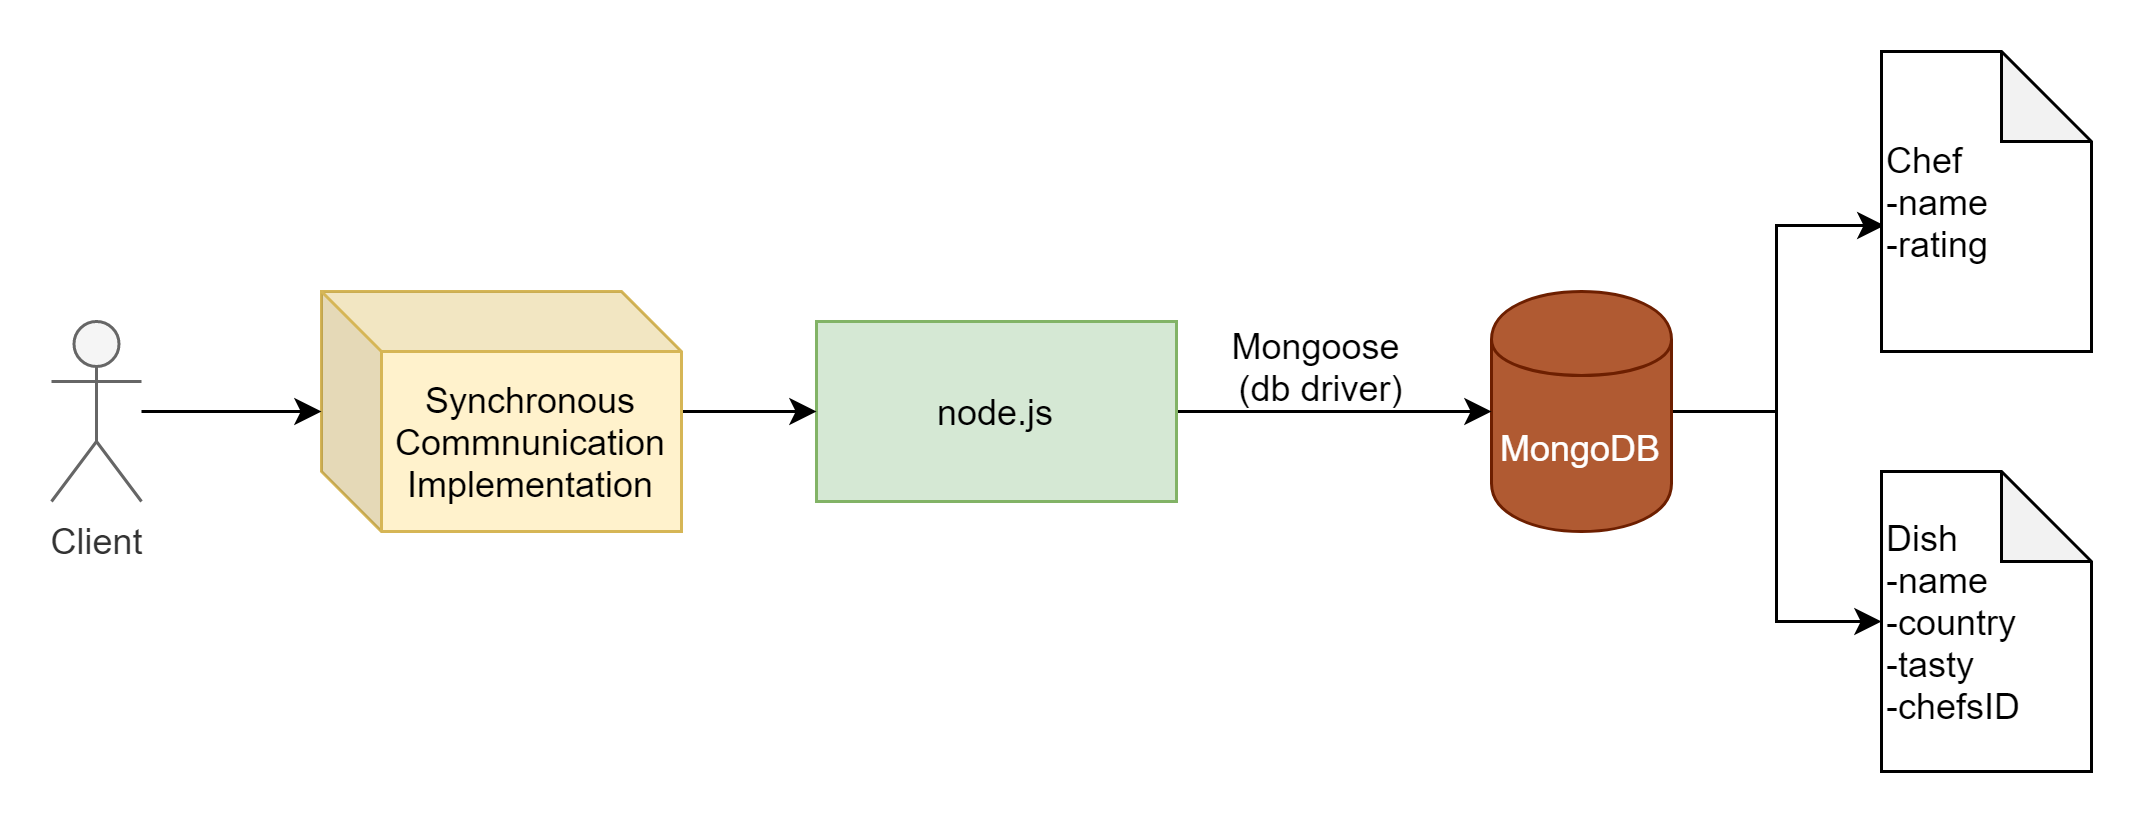
\includegraphics[width=\textwidth, height=0.8\textheight, keepaspectratio]{prototype_sync_comm_overview.png}
	\caption{Prototype setup for synchronous communication}
	\label{img:prototypesynccomm}
\end{figure}

\pagebreak
\textbf{RESTful HTTP}

The prototypic implementation of RESTful \ac{HTTP} endpoints is implemented with the popular server-side web framework \enquote{express.js}.
However, it should be noted that a native implementation of REST is possible with only built in functionalities of \textit{node.js}.
Apart from that, there are also many different middlewares available, such as \textit{sails.js} which make REST modular in its implementation.

The modularity is given because the endpoints are separated from each other.
In the prototypic implementation for example, handler for dishes and chefs are treated individually by their own routes, actions, and call paths (\enquote{http://host/dish} and \enquote{http://host/chef}).
In combination with proxies/gateways the different services can be exchanged, but still be served externally at the same location.

\begin{figure}[h]
	\centering
	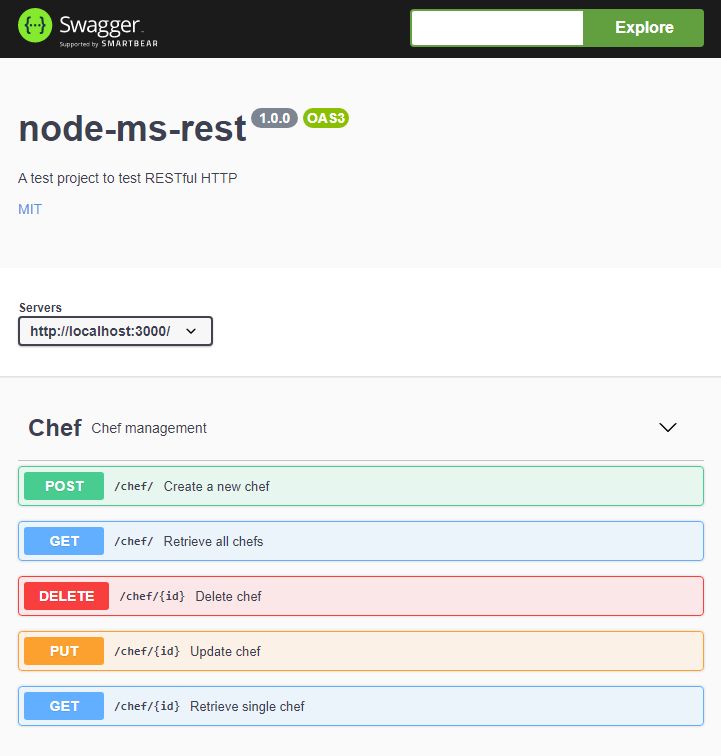
\includegraphics[width=\textwidth, height=0.4\textheight, keepaspectratio]{prototype_rest_swagger.png}
	\caption{Swagger/OpenAPI documentation of the prototypic REST implementation}
	\label{img:prototyperestswagger}
\end{figure}

With \textit{express.js} the learning effort from starting with an existing backend with database connection (cf. Figure \ref{img:prototypesynccomm}) to the first successful REST call was rather low.
This is due to the simplicity that frameworks usually entail.
Although they have a simple syntax, the concept of routing calls and the definition of endpoints must be learned.
As already alluded to in chapter \ref{cha:Technologies:communication:synchronous}, REST itself neither provides strong typing, nor any implementation constraints or specifications to be followed.
While this does offer development flexibility and initial simplicity, the developer and operator must agree on how to access the endpoint.
A basic example of such an agreement is the correct use of \ac{HTTP} verbs as defined in the Richardson Maturity Model (i.e. \textit{DELETE} for deleting resources, \textit{GET} for fetching) \cite{Fowler.2010}.
Consequently, the learning effort increases with the rising application needs, since the introduction of concepts such as hypermedia (i.e. HATEOAS) or versioning may lead to a greater change than with GraphQL.

Since REST itself is only an architectural design introduced by Fielding and later adopted into the \textit{Web Services Architecture (W3C)} and thus subject to the preferences of the developers, there is still no clear definition or \enquote{correct} documentation available on how to implement it \cite{Fielding.15.03.2002}\cite{W3CWorkingGroup.2004}.
Furthermore, there is no clear de facto standard yet, which makes it difficult to define whether an implementation is truly a REST endpoint.
On the other side however, it is common to still benefit from the flexibility, but document the resulting (custom) implementation through specification standards such as \textit{OpenAPI} (or formerly known as \textit{Swagger Specification}).
A screenshot of one of the implemented \textit{Swagger} documentation in the prototype is shown in Figure \ref{img:prototyperestswagger}, where possible operations and the REST endpoints are listed.
Moreover an example call triggered over the web interface of the documentation can be seen in Figure \ref{img:prototyperestcall}.

Apart from concrete \textit{HTTP} client implementations in any programming language, such as \textit{Axios} for JavaScript environments, and the aforementioned documentation tools  there are no other noteworthy extensions for a RESTful \ac{HTTP} service.

\begin{figure}
	\centering
	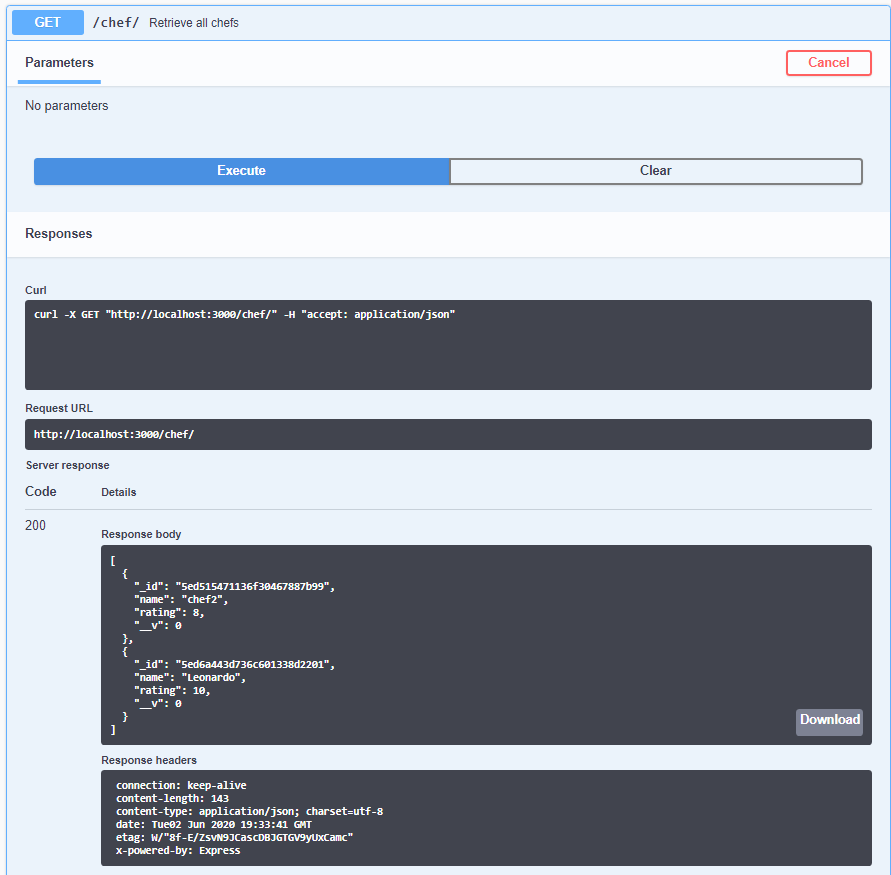
\includegraphics[width=\textwidth, height=0.45\textheight, keepaspectratio]{prototype_rest_swaggercall.png}
	\caption{Exemplary REST call to fetch all chefs using \textit{Swagger}}
	\label{img:prototyperestcall}
\end{figure}

\pagebreak
\textbf{GraphQL}

Similarly to the previous prototype, \enquote{express.js} is used in conjunction with the officially recommended \enquote{express-graphql} connector.
The latter provides options to build the schema for the GraphQL endpoint either with an own language or with JavaScript.
Furthermore, a connector provides an interactive in-browser \ac{IDE} (\enquote{\textit{GraphiQL}}) for executing queries, which includes schema browsing.
As GraphQL is only a specification, other server alternatives to \textit{express-graphql} exist, such as the \textit{Apollo} server.

\begin{figure}
	\centering
	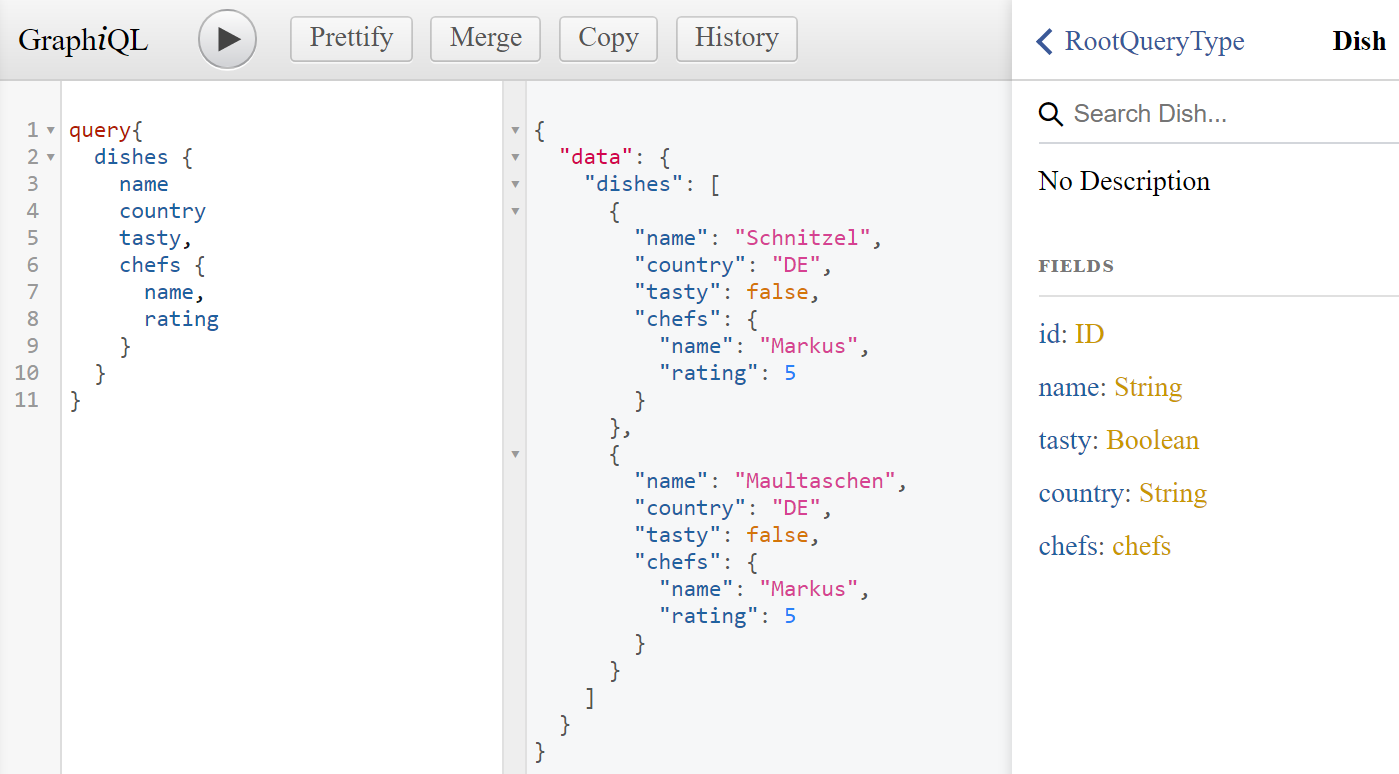
\includegraphics[width=\textwidth, height=0.5\textheight, keepaspectratio]{prototype_graphql_graphiql.png}
	\caption{Exemplary GraphQL call to fetch all dishes and corresponding chefs using \textit{GraphiQL}}
	\label{img:prototypegraphiql}
\end{figure}

For the prototypic implementation, the focus was on implementing a GraphQL \ac{API} handler that accepts queries over a \ac{HTTP} endpoint.
Consequently, any \ac{HTTP} enabled client can access the GraphQL backend without much implementation effort.
However, it should be noted, that for production environments more complex clients, which may include batching, caching and other optimizations, exist and should be used (e.g. \textit{Apollo} client).
With the current implementation, an exemplary query (as shown in Figure \ref{img:prototypegraphiql}) can be executed, either with a \textit{POST} \ac{HTTP} call or by using \textit{GraphiQL}.
As already outlined in chapter \ref{cha:Technologies:communication:synchronous}, although the same database is used as in the previous prototype, GraphQL allows the client to retrieve only the needed information, including nesting (i.e. retrieve attributes from chefs connected to the dish in this example).

Regarding modularity, there is no native support for splitting  a GraphQL instance and its underlying scheme definition, thus providing modularity.
However, for officially referenced toolsets that were not part of this prototype, \enquote{schema stitching} is one way to achieve modularity.
Figure \ref{img:prototypegraphqlproxy} shows how multiple GraphQL servers can be combined with each own database connection and scheme, even together with different RESTful \ac{HTTP} endpoint, allowing the client to submit a query to a single GraphQL endpoint.

The extension \textit{graphql-tools} for stitching is only one of many available extensions for GraphQL.
Besides the plethora of available client and server implementations for each programming language, third party libraries and tools are also available.
Examples are a content management system (\textit{graphcms} or \textit{tipe}), visualization tools (\textit{graphql voyager}), documentation platforms \textit{GraphQL Docs} and the popular fullstack platform \textit{Apollo}.
Consequently, although GraphQL is not as simple as a RESTful \ac{API}, its widespread support makes it very flexible.

\begin{figure}[h]
	\centering
	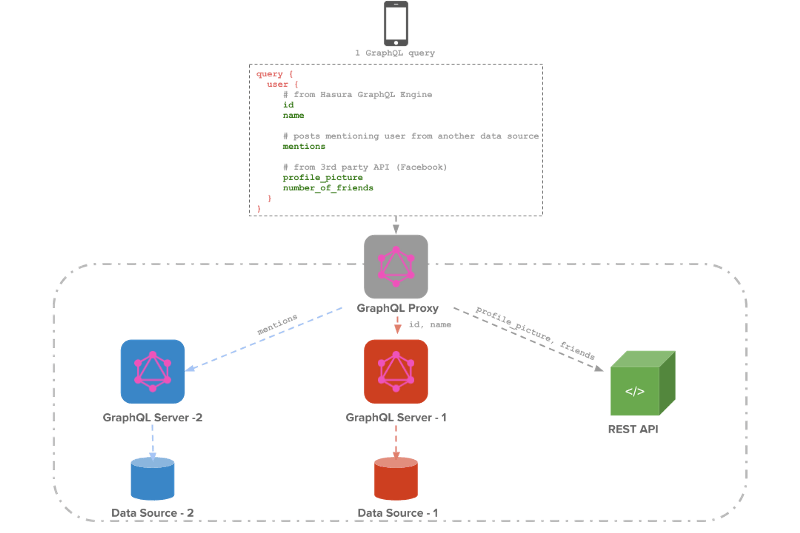
\includegraphics[width=\textwidth, height=0.3\textheight, keepaspectratio]{prototype_graphql_proxy.png}
	\caption{Combining different data sources - schema stitching using \textit{graphql-tools} extension \cite{Wawhal.2018}}
	\label{img:prototypegraphqlproxy}
\end{figure}

GraphQL itself mostly provides reference implementations that are officially documented but are often superceded by third party implementations.
All concepts, scheme language definition and best practices are documented extensively on the official website.
This includes the \ac{API} reference for reference implementations (in this case \textit{graphql-js}), on which additional libraries, such as the one used in the prototype are built upon (\textit{express-graphql}).
On the contrary, as third party implementations are often used due to their ease of use and simplification, the practical usage of GraphQL may be bound to external documentation, making a general statement about the level of documentation of GraphQL difficult.

Nevertheless, the documentation is helpful in learning how to use GraphQL.
As the schema language, typing and the general concept of queries and mutations must be learned to use GraphQL, the learning effort is to be rated as moderate.
While documentation is available, the learning curve may be steep at first due to the new concepts, especially when never having dealt with graph-based databases before.

\textbf{Conclusion}

As expected, REST is easier to implement due to its loose specification, while GraphQL presents itself as a well thought-out and exhaustive framework with many features, but which requires learning initial concepts.
The synchronous communication in the exemplary LAN party application will mostly be found in communication of the web-based frontend with the backend services instead of the inter-service communication.
This circumstance does not exclude the possibility of using GraphQL or REST in the backend.
However, in this application, the publish-subscribe pattern with asynchronous communication may be suited better, which is why the evaluation focuses on the frontend communication.

For the final implementation, REST is selected because of the lower learning effort and the broad and simple compatibility.
Especially for the client side, which is a web browser in this case, it is easier to implement a connection to the REST \ac{API}, than with GraphQL, which often needs more than a simple \textit{POST} request, but rather client tooling for maintainability and performance.
Although the clients in this use case are performant enough to be more than \textit{thin clients} and could handle more complex operations, REST is more sensible here.
There are very few cases where data needs to be retrieved, manipulated or actions need to be triggered which GraphQL would perform better.
Such a possible feature would be, for example,  browsing for teams in the scoreboard and displaying recent matches of the team.
Although this would be a feature where GraphQL would excel, other, less complex features would have to be built with the same amount of complexity compared to REST.

Nevertheless, GraphQL, with its contract-driven design, introspection, and thus consistent endpoint and schema declaration, clearly overshadows REST for moderate and complex operations.
However, in the context of the LAN party application, the effort needed to achieve the aforementioned benefits is unjustifiable compared to the actual, relatively simple needs covered by REST.
Finally, however, as GraphQL can and is often used on top of existing (cf. chapter \ref{cha:Technologies:communication:graphql}) REST \acp{API}, an extension at a more developed stage of the LAN party application should be taken into consideration, in order to benefit from GraphQL's features, while providing REST alongside in a hybrid approach.


\clearpage
\section{Asynchronous Communication RabbitMQ and Apache Kafka}\label{cha:Implementation:async}
%!TEX root = ../../dokumentation.tex

Both \textit{RabbitMQ} and Apache \textit{Kafka} (hereinafter \enquote{Kafka}) use the same initial setup for prototyping, as shown in Figure \ref{img:prototypeasynccomm}.
The task is to create a topic where ten consumer are subscribed to and each published message from the producer is send to each consumer.
A total of 10000 messages will be sent via the implemented solution, and the consumer checks if the order of the messages was correct.
The time for sending and receiving all messages will be measured.
It should be noted that the measured times will only be used to get the gist of the transmission speeds.
\textit{node.js} will be used for implementation because it is well suited for microservice architecture \cite{AnkitKumar.2019} and has already been used in the prototype for synchronous messaging.
Two \textit{node.js} services are created, and automated with \textit{docker} and \textit{docker-compose}.
The \textit{docker-compose} will also contain the messaging infrastructure.

\begin{figure}[h]
	\centering
	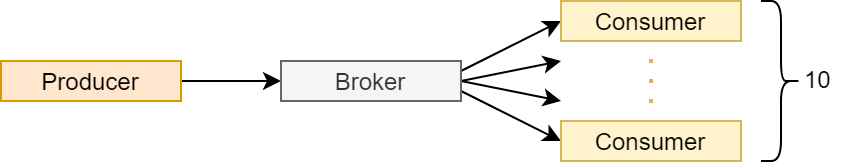
\includegraphics[width=\textwidth, height=0.8\textheight, keepaspectratio]{proto_async.png}
	\caption{Prototype setup for asynchronous communication}
	\label{img:prototypeasynccomm}
\end{figure}

\textbf{RabbitMQ}

The prototypic implementation of \textit{RabbitMQ} will use the \ac{AMQP} protocol as it is the default option.
The consumer and producer services use the \textit{amqplib} library to connect to \textit{RabbitMQ}.
There are other library options, but \textit{amqplib} is the most downloaded one on \textit{npm} \cite{npmtrends.2020}.
\textit{RabbitMQ} also provides an official docker image which was used for this prototype.

The modularity is given since exchanges and queues can be freely defined within the code or via a management interface.
In the prototype, both are created within the code, but this creates coupling between producer and consumer.
The coupling between producer and consumer is shown in Figure \ref{img:rabbitmqproto} by the brackets in the respective color of the producer and consumer.
The producer knows only the exchange definition, while the consumer knows exchange and queue definitions.
It is important to note, that this coupling can be reduced if the exchange and queues are defined via the management interface.

\begin{figure}
	\centering
	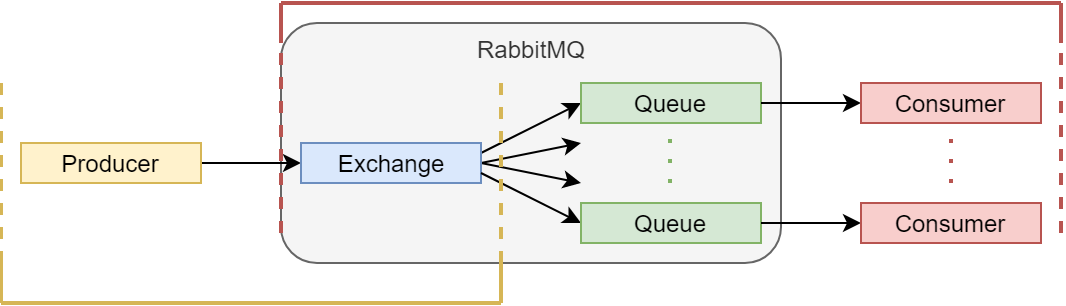
\includegraphics[width=\textwidth, height=0.9\textheight, keepaspectratio]{rabbitmq_proto.png}
	\caption{RabbitMQ prototype implementation}
	\label{img:rabbitmqproto}
\end{figure}

Apart from that, the learning effort for creating the prototype was rather low.
Setting up the \textit{RabbitMQ} instance was straight forward with the official \textit{docker} image and connecting the producer and consumer to the instance was easy due to the code examples from \textit{amqplib}.
However, a lot of repetitive code is required when a consumer connects to multiple queues.
In this case, it would make sense to create a management component.

As mentioned above, the available documentation of \textit{amqplib} contains code examples \cite{MichaelBridgen.25.04.2018}, as well as an extensive \ac{API} documentation \cite{MichaelBridgen.14.05.2020}.
\textit{RabbitMQ} also has extensive documentation available on there homepage, which also explains the concepts of \ac{AMQP} and more.
Since the standard \ac{AMQP} is used, a standard way to implement the communication is provided.
On the contrary, since it is specified by protocol, the available amount of extensions is rather low.
Of course, \textit{RabbitMQ} provides plugins to support \ac{MQTT} and \ac{STOMP}, but otherwise there is very little available.
For \textit{node.js} its the same, there are only different implementations for the protocol or wrapper projects to provide TypeScript support.

\textbf{Apache Kafka}

The prototypical \textit{Kafka} implementation includes a producer and consumer service that use the library \textit{KafkaJS} to connect with \textit{Kafka}.
\textit{KafkaJS} has gained popularity over the last year and is slowly closing the gap to the most popular library \textit{kafka-node}.
These two library's are the most used once \cite{npmtrends.2020b}.
Initially, the prototype used \textit{kafka-node}, but it did not work as planned.
In addition, there is no official \textit{Kafka} \textit{docker} image,  so a few were tested.
The \textit{docker} image \textit{wurstmeister/kafka} was chosen because it is the most used \textit{Kafka} \textit{docker} image on \textit{www.docker.hub} \cite{DockerInc.05.06.2020} and is well documented.
It is important to note that while using \textit{kafka-node}, the \textit{Kafka} image was not fully functioning.
Therefore, it is likely that it would work now, after ensuring that the \textit{Kafka} image works as intended.
Finally, for the official \textit{docker} image of \textit{zookeeper} was used.

This now leads to the actual implementation, which is shown in Figure \ref{img:kafkaproto}.
As in the \textit{RabbitMQ} prototype, only one topic was created.
Normally, to enhance the throughput, multiple partitions within one topic would be used, but when using multiple partition, there is no message ordering guarantee.
The ordering of message is guaranteed only within one partition and not within one topic \cite[p.~30]{Kumar.2017}.
The coupling between producer and consumer is much lower compared to \textit{RabbitMQ}.
Both only need to know the topic name.
The figure also shows that each consumer belongs to a separate consumer group.
This is necessary so that each of the ten consumers receives the messages.

\begin{figure}[h]
	\centering
	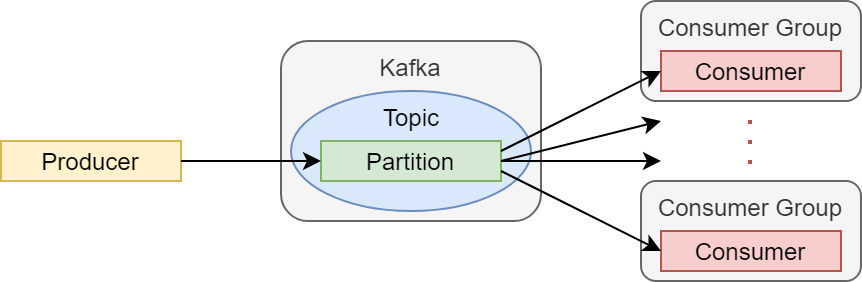
\includegraphics[width=\textwidth, height=0.9\textheight, keepaspectratio]{kafka_proto.png}
	\caption{Apache Kafka prototype implementation}
	\label{img:kafkaproto}
\end{figure}

This results in a higher learning curve than with \textit{RabbitMQ}.
This is mainly because there is no official \textit{Kafka} \textit{docker} image and both the documentation form \textit{wurstmeister/kafka} and \textit{KafkaJS} are extensive and thus it takes time to understand them.
The implementation of the \textit{Kafka} prototype took twice as long as with \textit{RabbitMQ} because the steeper learning curve.
As mentioned above, the documentation available for the used \textit{Kafka} \textit{docker} image and library are extensive.
In case of \textit{KafkaJS}, it contains code examples for getting started as well as a complete description of the producer and consumer functionality and more complex features such as transactions \cite{TulioOrnelas.2020}.
There is also the official \textit{Kafka} documentation to get a more detailed insight about \textit{Kafka} \cite{ApacheKafka.01.06.2020}.
In this prototype, no extensions for \textit{Kafka} were used, but there are some available.
As already explained in \ref{cha:Technologies:communication:kafka}, \textit{Kafka} is the perfect base for an \textit{Event Sourcing} system \cite[p.~19]{Stopford.2018}.
The \textit{AxonFramework} extension aims to extend \textit{Kafka} to provide a framework that can be used to create evolutionary, event-driven microservice systems, based on the principles of Domain Driven Design, Command-Query Responsibility Segregation (CQRS) and Event Sourcing \cite{StevenvanBeelen.29.05.2020}.
Another extension to connect \textit{Kafka} with \textit{Azure} is being created by \textit{Microsoft} \cite{Microsoft.28.05.2020}.
Both extensions are still in the beta phase.
Finally, \textit{Kafka} provides complete freedom in the serialization of data send over or stored within \textit{Kafka}.
The library \textit{Avro} is often used in combination with \textit{Kafka} \cite{JayKreps.2015}.

\textbf{Conclusion}

After implementing a prototype for both asynchronous messaging technologies, the subjective conclusion is that \textit{RabbitMQ} is easier to use.
The main reason are the instructions in the documentation and the provided official \textit{docker} image from \textit{RabbitMQ}.
This made it easy to implement the prototype quickly.
On the other hand, \textit{Kafka}, with its rather complex setup, has a higher skill sealing.
The missing official \textit{docker} image was an issue because every \textit{Kafka} \textit{docker} image must be used sightly different, which leads to search for the right approach.
In the \ac{LAN} application, the required functionality is publish-subscribe to synchronize the microservices.
Therefore, a ordering guarantee and the \ac{QoS} type \textit{at-least-once} are required.

Both Technologies meet the requirements and therefore a benchmark was conducted to evaluate which technology performs better in the given task.
The full benchmark results can be found in the appendix at \ref{chp:appendix:benchmark}.
\textit{RabbitMQ} was significantly faster than \textit{Kafka}.
As a result, \textit{RabbitMQ} was chosen for the \ac{LAN} application because it is faster and easier to use than \textit{Kafka}.


% Example LAN App
%!TEX root = ../dokumentation.tex

\chapter{Example LAN Application Implementation}\label{cha:ExampleLAN}

To develop an application, a plan is required that guides the development process, which is usually at least an architecture concept.
The architecture is created based on the application components (cf. chapter \ref{cha:Requirement:lanpartyapplication}) and the technologies selected (cf. chapter \ref{cha:Implementation}).
To fully exploit the potential of the technologies, the resulting \ac{LAN} Application will be implemented using the microservice architecture.
An important principle is the single responsibility principle form Robert C. Martin’s: \cite[p.~4]{Bruce.2019}

\begin{quote}
	Gather together the things that change for the same reasons. Separate those things that
	change for different reasons.
\end{quote}

Taking this principle into account and combining it with the application components, each component will be isolated into its own microservice.
Other microservice attributes that should be considered are, for example, that a microservice should know little about other microservice, they should be independently deployable and replaceable.
These attributes leads to providing one database per microservice \cite[p.~4ff.]{Bruce.2019}.

Another important part to consider when building a microservice architecture it the fact that it is a distributed system.
False assumptions like the network is reliable must be avoided \cite[p.~16]{Bruce.2019}.
Therefore, \ac{QoS} \textit{at-least-once} will be used and considered when creating the architecture.
It was chosen because the application must be consistent and availability can be achieved by scaling.

These are the general guidelines for creating the architecture, next is to evaluate the use of the different communication technologies.
The selected technologies are \ac{REST} for synchronous messaging and RabbitMQ for asynchronous messaging.
Synchronous messaging is used for communication where direct feedback is required, such as client-server communication.
Asynchronous messaging, on the other hand, is used to decouple communication partners.
This allows dynamic growth and parallel work distribution within the microservice application \cite[p.~62f.]{Bruce.2019}.
Therefore, asynchronous messaging is used for inter-service communication.

Another common principle in microservice architectures is the use of a boundary layer that provides abstraction over internal complexity and change \cite[p.~66]{Bruce.2019}.
Therefore, an \ac{API} Gateway will be used as single entry point for the application.
This has advantages such as centralized handling of authentication, routing and transmission transformations.
It also minimizes the exposed surface area of the application \cite[p.~68f.]{Bruce.2019}.

Now that the general structure of the services has been described, one last part must be described, namely the \ac{UI}.
The user interface can be either a web page or full fledged application, and both can be implemented via a monolith or micro frontend approach.
The \ac{UI} will have cross microservice concerns to ensure usability \cite[p.~71f.]{Bruce.2019}.
So, since this work focuses on communication technologies for a microservice environment, the approach used for the \ac{UI} should hardly affect communication.
Therefore, a monolithic web page will be realized because it is simple to realize, and the authors have experience with this kind of application.

The architecture of the \ac{LAN} application can be divided into two parts.
The first part shows the synchronous communication and the second part shows the asynchronous communication.

\textbf{Overview of the Synchronous Messaging Architecture}

An architectural overview of the synchronous messaging is shown in Figure \ref{img:lansyncoverview}.
An \ac{API} gateway, which will be \textit{Nginx}, abstracts the microservice system.
Depending on the domain used, \textit{Nginx} forwards the requests to the microservice system or to \textit{Grafana}.
This means that \textit{domain.de} will return the \ac{LAN} application and \textit{metric.domain.de} will return \textit{Grafana}.
Each microservice has its own REST endpoint which is accessible via \textit{/api/<name of service>}.
\textit{Nginx} will use the service name within the \ac{URL} to route the request and truncate the \ac{URL}.
For example, a request \textit{domain.de/api/account/1} will be routed to the account microservice and the forwarded request will be \textit{<ip of account>/1}.

For logging purposes, Prometheus will be used.
Each microservice will collect metrics about requests and provide an endpoint for Prometheus.
This is visualized by the red box attached to each microservice.
Finally, each microservice has its one MongoDB database.
For simplicity, all databases run in one instance, but they could be distributed across different MongoDB instances.

\begin{figure}
	\centering
	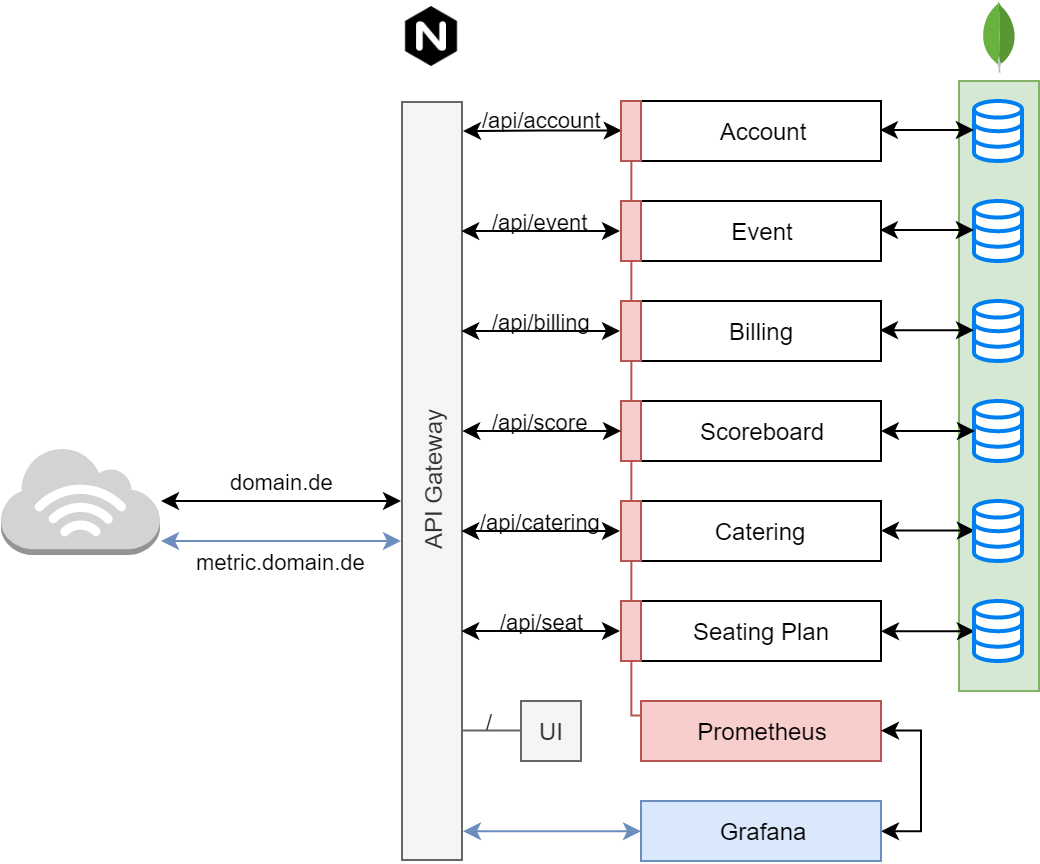
\includegraphics[width=0.7\textwidth, height=0.9\textheight, keepaspectratio]{LAN_Application_REST.png}
	\caption{LAN application synchronous messaging architecture overview}
	\label{img:lansyncoverview}
\end{figure}

\textbf{Asynchronous Messaging Events}

Before describing asynchronous messaging, it is important to note that every microservice must be able to validate any request from the client by itself.
Therefore, the microservice needs the necessary information for any validation itself and must not be dependent on other microservice.
This leads to the distribution of shared information and that is the main concern of the following overview of asynchronous messaging.

Figure \ref{img:lanasyncevents} is a simplified overview of the available topics and how the microservices interact with them.
An important design decision was made to allow the flexibility described above.
Every microservice must subscribe to the \textit{Account} and \textit{Event} topics, to receive all \textit{created} events (not included in the image for readability).
This distributes the event and account ID's to all microservice.
These ID's are the center of almost all operation.

In Figure \ref{img:lanasyncevents}, most of the publish arrows numbered.
Each number is associated with a reason for this connection, which is described in the following list.
\begin{enumerate}
	\item \textit{Events} and \textit{catering} can cost money and must therefore inform \textit{billing}
	\item The \textit{event} must know when the fees for an event are payed
	\item The \textit{catering} and \textit{searing plan} must know when an account has registered for an event. This will enable there functionality.
	\item The \textit{scoreboard} must know when an event starts and when it ends
	\item \textit{Scoreboard} publishes a summery of the event results to event and account topics
\end{enumerate}

\begin{figure}
	\centering
	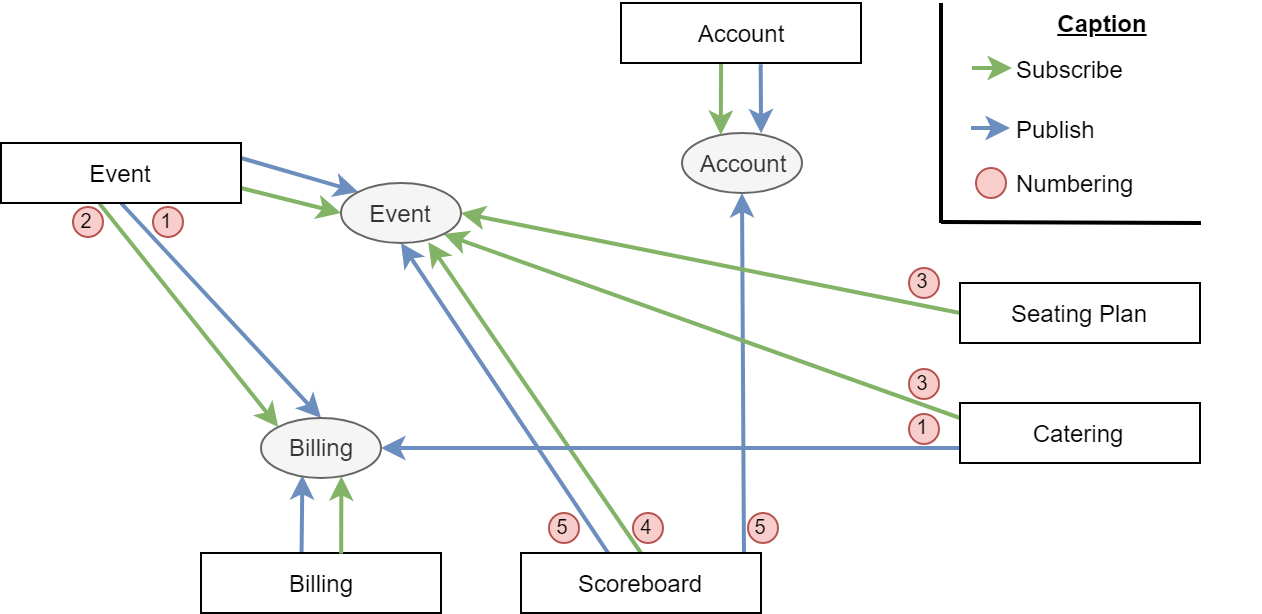
\includegraphics[width=0.9\textwidth, height=0.9\textheight, keepaspectratio]{LAN_Application_Events.png}
	\caption{LAN application asynchronous messaging events overview}
	\label{img:lanasyncevents}
\end{figure}

This concludes the architecture overview of the \ac{LAN} application.
It is important to note that this was only a high-level overview of the actual application.

\textbf{Implementation Details}

For the actual implementation, the following extensions/frameworks are used in addition to the selected technologies mentioned above:

\begin{enumerate}
	\item \textbf{express.js}: Server-side web framework for node.js (version \textit{4.17.1})
	\item \textbf{mongoose}: MongoDB object modeling framework for node.js (version \textit{5.9.17})
	\item \textbf{amqp-ts}: \ac{AMQP} communication library for node.js (version \textit{1.8.0})
	\item \textbf{bcryptjs}: Password hashing library for node.js based on \textit{bcrypt} (version \textit{2.4.3})
	\item \textbf{express-jwt}: Middleware for validating \ac{JSON} Web Tokens (version \textit{5.3.3})
	\item \textbf{Angular}: Web application framework for frontends (version \textit{9.1.9})
	\item \textbf{ng-Bootstrap}: Widgets for \textit{Angular} based on \textit{Bootstrap}, a styling framework (version \textit{6.1.0})
\end{enumerate}

In contrast to the presented services in Figure \ref{img:lansyncoverview}/\ref{img:lanasyncevents}, only three services are implemented, namely \textit{Event},\textit{ Account} and \textit{Billing}.
Although the resulting implementation would not be a viable application for an actual LAN party, it was important to demonstrate the underlying architecture for communication and event flow.
Consequently, it can be extended with additional services without many changes.

Each implemented service is bundled into an image using \textit{Docker}, which allows containerization and flexible deployment via a \textit{docker-compose} script that also handles switching environments (e.g. for development).
The current implementation consists of the following services:
\begin{enumerate}
	\item Nginx
	\item MongoDB
	\item RabbitMQ
	\item Prometheus
	\item Grafana
	\item Each implemented node.js service:
	      \subitem Account
	      \subitem Event
	      \subitem Billing
\end{enumerate}

As alluded in Figure \ref{img:lansyncoverview}, each external request is forwarded using \textit{Nginx}, including access to additional informative services (\textit{mgnt} subdomain), such as \textit{Grafana}, and direct database access (separate port) to \textit{MongoDB}.
However, the backend communicates with said services through internal endpoints, since each service is located on the same isolated network provided by \textit{Docker}.
Consequently, metric reporting and database access is restricted to the microservice environment itself.
Although metrics are already collected through Prometheus and accessible via \textit{Grafana}, a dashboard implementation was omitted in \textit{Grafana}.

Apart from the REST communication to the frontend, there is also inter-service communication over \ac{AMQP}.
The binding selected for connecting a queue to an exchange entity is a regular expression (topic exchange).
Each event has its own expression to synchronize with the services, such as \textit{account.created}, which means that the main topic is \enquote{account} and the associated sub topic is \enquote{created}.
Furthermore each service listening/consuming a queue is implemented in a way that same events can be received more than once, but only the first time is of relevance.
This implementation detail is important, as the implementation of the \ac{AMQP} protocol in this work uses a \textit{at-least-once} \ac{QoS}.

An exemplary flow of both synchronous and asynchronous messages across the whole architecture is shown in Figure \ref{img:registeraccountevent_sequence}.
The synchronous calls over REST are highlighted in blue, whereas the asynchronous publishing of messages using \ac{AMQP} are highlighted in orange.
Moreover, the data sent in each step is also shown, whereas not all internal functions of each service are represented here .
For a complete list of implemented and used events, as well as available REST endpoints, see \ref{chp:appendix:implementedRest} and \ref{chp:appendix:implementedEvent} in the appendix.

\begin{figure}
	\centering
	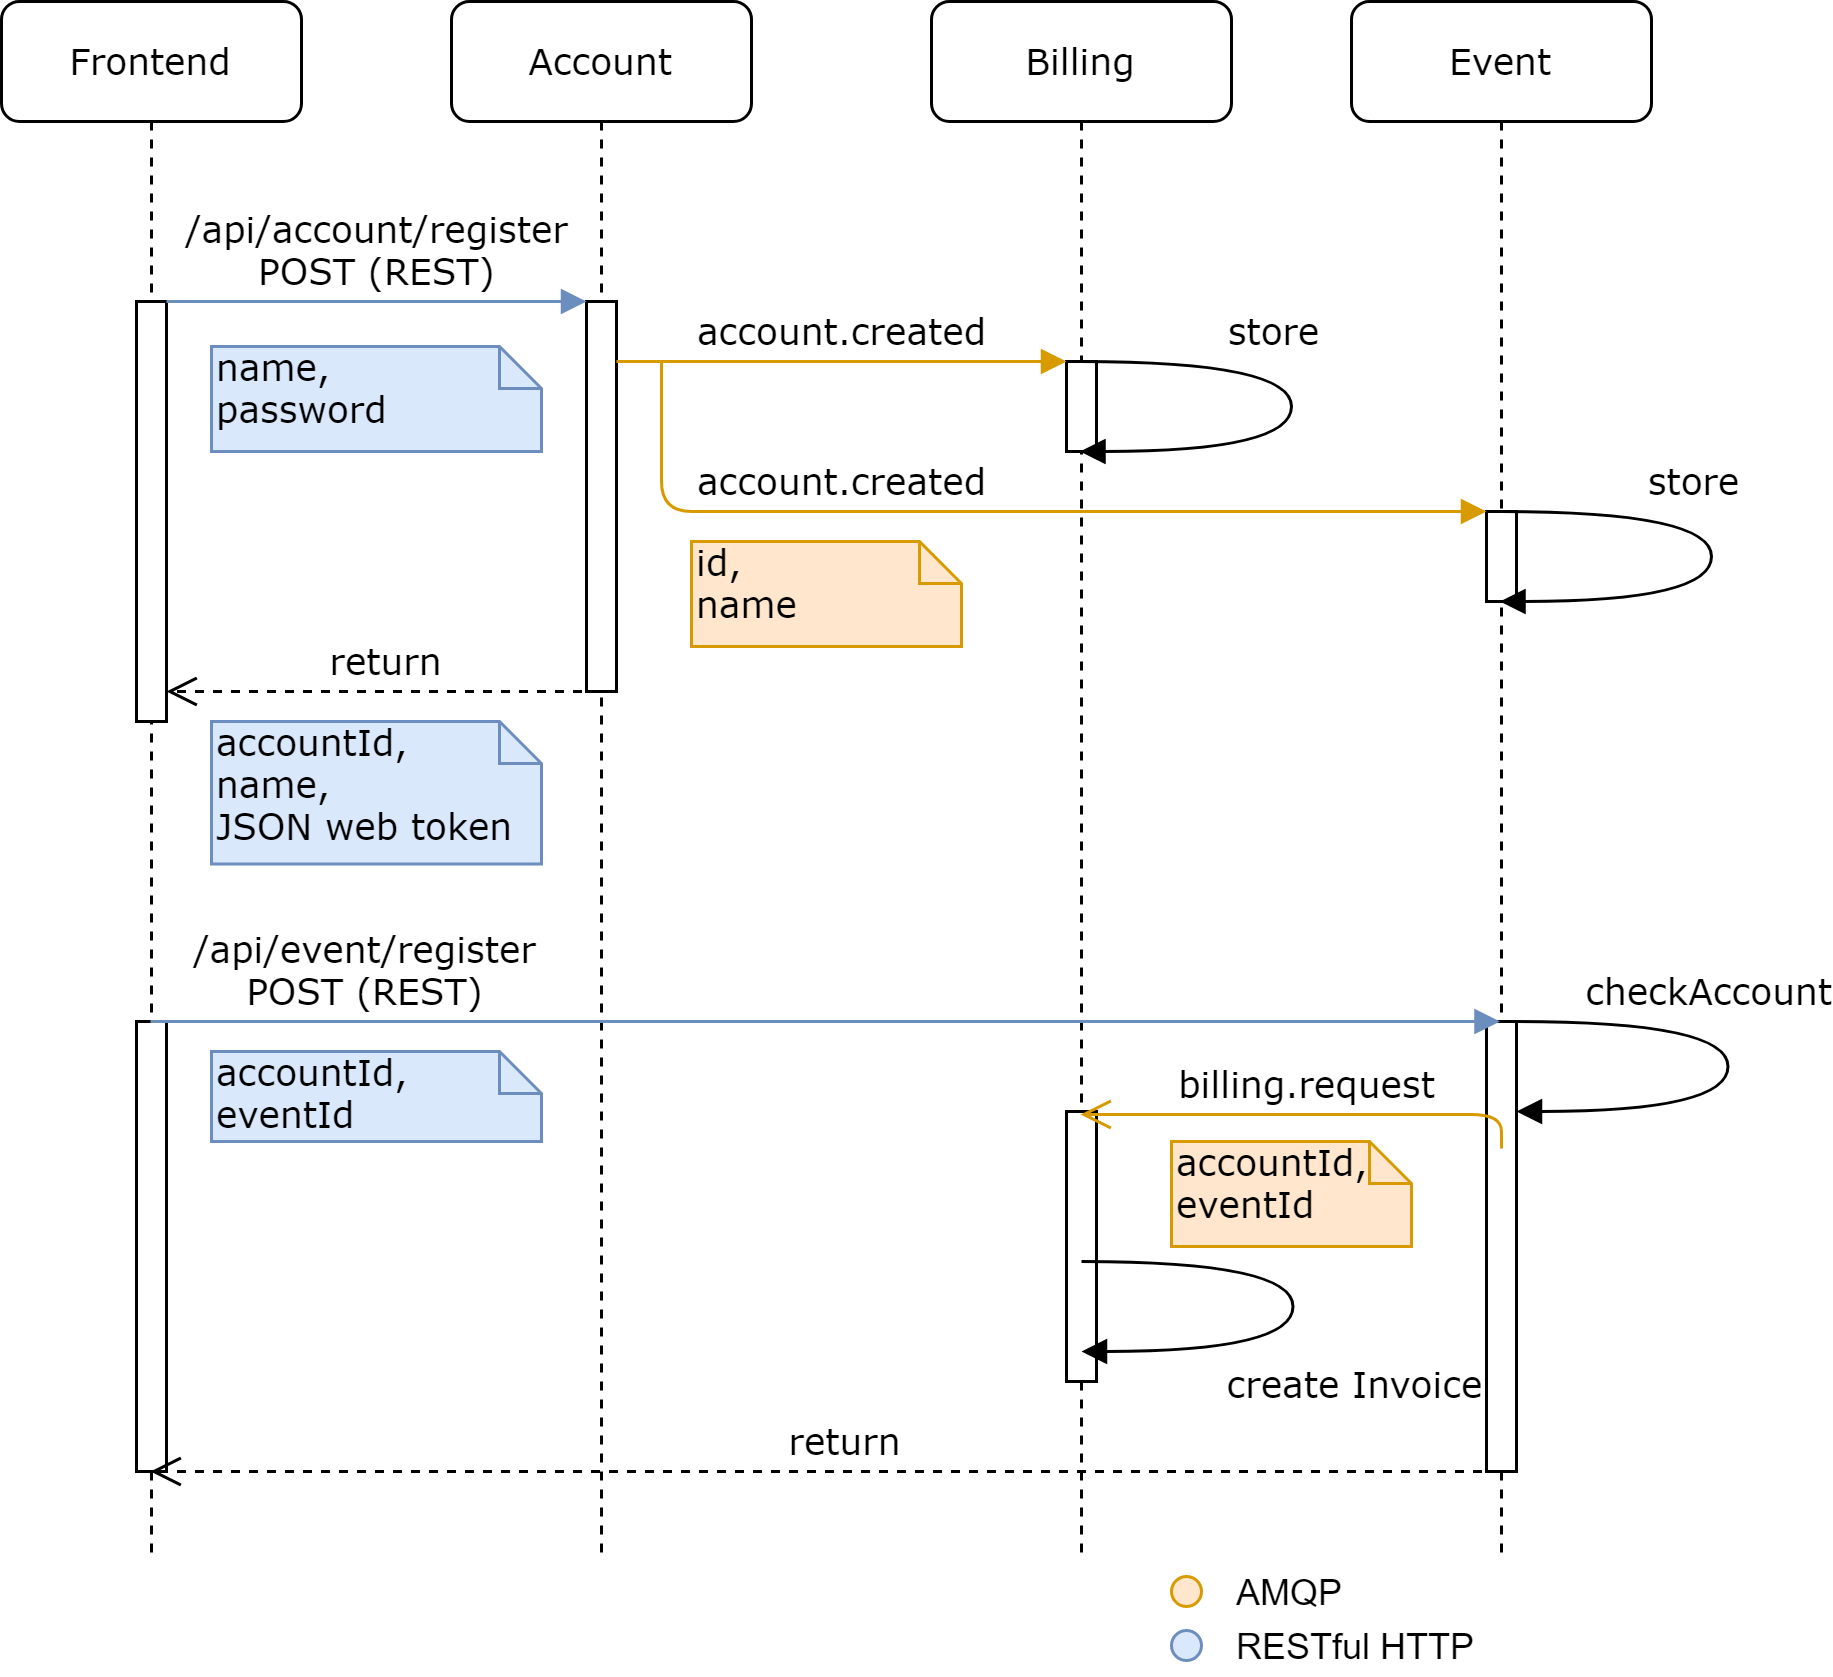
\includegraphics[width=\textwidth, height=0.6\textheight, keepaspectratio]{registeraccountevent_sequence.png}
	\caption{Example of registering account and registering for an event}
	\label{img:registeraccountevent_sequence}
\end{figure}


% Fazit
%!TEX root = ../dokumentation.tex

\chapter{Conclusion}\label{cha:Conclusion}

With an increasing number of different libraries, frameworks and technologies in general, each attempting to better solve an existing problem, this work is likewise an approach to solve the problem of deciding between said technologies, by providing an overview and disclosing the thought process.
This work introduces a selection of available technologies in the field of communication and monitoring, key aspects in driving a microservice architecture.
In order to evaluate the features included in each framework, prototypical implementations were used to attain further insights for the final selection.

Apart from the proof-of-concept implementations performed in chapter \ref{cha:Implementation}, the general requirements in a microservice environments are a key factor in shaping the selection.
Consequently, practical experience was taken into consideration by conducting expert interviews, that showed that performance is one of the highest requirements for most of the personas presented in the requirement analysis.
For the selection of technologies to be used in the exemplary LAN party application, \textit{RabbitMQ} was selected over \textit{Apache Kafka} for asynchronous inter-service communication, \textit{RESTful HTTP} over \textit{GraphQL} for synchronous frontend communication.
Lastly \textit{Prometheus} was favored over \textit{Graphite}.
An overview of each of the three aspects, including technologies that were considered unsuitable for this application, can be found in chapter \ref{cha:Technologies} in the tables \ref{tab:overviewSynchronousCommunication} [p. \pageref{tab:overviewSynchronousCommunication}], \ref{tab:overviewAsynchronousCommunication} [p. \pageref{tab:overviewAsynchronousCommunication}] and \ref{tab:comparisonmonitoring} [p. \pageref{tab:overviewAsynchronousCommunication}] respectively.

Naturally, the selection is not complete and not all features were covered in the proof-of-concepts.
Nonetheless, the selection made in chapter \ref{cha:Implementation} allowed for a fast implementation and confirmed the interoperability of the services using the technologies.


\textbf{Outlook}

After considering several communication and monitoring technologies, comparing several prototypes and building an exemplary application, the question remains open as to how to proceed further.
Other topics such as gateways and message tracing still need to be compared.
Popular gateways are for example \textit{Gateway-Apache} and \textit{Nginx}, which could be compared based on modularity, learning effort, available documentation and available extensions, like the prototypes of this work.
The same applies for tracing, where \textit{Jaeger} and \textit{Zipkin} are popular.
But there are also other fields than communication, such as \textit{code generation}, \textit{automatization} and \textit{static code analysis}, that leave room for comparison.

Finally, although the exemplary application was not completed, it still provided a deeper insight into the practical use of communication technologies.
All in all, the foundation can be considered as completed, while other aspects for a complete and coherent product are missing.



% Inhalt
%\foreach \i in {01,02,03,04,05,06,07,08,09,...,99} {%
%	\edef\FileName{content/\i kapitel}%
%		\IfFileExists{\FileName}{%
%			\input{\FileName}
%		}
%		{%
%			%file does not exist
%		}
%}

\clearpage

\pagenumbering{roman}

% Literaturverzeichnis
\cleardoublepage
\printbibheading
\printbibliography[nottype=online,heading=subbibliography,title={Publikationen}]
\printbibliography[type=online,notkeyword=Gesetz,notkeyword=Standard,heading=subbibliography,title={Online Quellen}]
\printbibliography[type=online,keyword=Gesetz,heading=subbibliography,title={Rechtsquellenverzeichnis}]
\printbibliography[type=online,keyword=Standard,heading=subbibliography,title={Standards \& Normen}]

%	\renewcommand\bibname{Literaturverzeichnis}
%	\printbibliography

%	\newpage\null\thispagestyle{plain}\newpage

% Glossar
\printglossary[style=altlist,title=\langglossar]

% sonstiger Anhang
\clearpage
\appendix
% !TeX root = ../dokumentation.tex

\addchap{\langanhang}

\chapter{Expert interviews}
\label{chp:appendix:interview}

Two expert interviews were conducted as part of this work.
The goal was to gain information on what is important as a member of a development team for a  distributed communication system.
This information was used to shape the developer and operator personas.

\paragraph{Developer interview}

The interview was conducted on the 20.05.2020 with an managing solution architect.
He has worked for 13 years, among others as software engineer and solution architect in projects with focus on API management, distributed architecture and integration systems.
This interview is the reference \cite{ManagingSolutionArchitect.20.05.2020}.

\paragraph{Operator interview}

The interview was conducted on the 20.05.2020 with an enterprise architect for cloud based infrastructure.
He has worked for 20 years, among others as project manager, lead architect and DevOps subject matter expert.
This interview is the reference \cite{EnterpriseArchitectforcloudbasedinfrastructure.20.05.2020}.

\pagebreak

\chapter{Benchmark of asynchronous messaging prototypes}
\label{chp:appendix:benchmark}

Each asynchronous prototype needed to handle 10000 messages from one producer and these were distributed to 10 consumers.
Both benchmark runs were executed on the same machine.
The results from RabbitMQ (\ref{listing:rabbitbenchmark}) show one transmission with a sending time of 283 ms and average receiving time of 4630,3ms.
In Apache Kafka there were three different producer implementations which were evaluated.
\begin{itemize}
    \item Type 1 (T1): each message was send and the response was immediately awaited.
    \item Type 2 (T2): all messages were send, the promises were collected in an array and all awaited at once with \textit{Promise.all()}
    \item Type 3 (T3): all messages were send and no response was awaited, except for the last response (which is the end signal)
\end{itemize}

The results from Apache Kafka are shown in \ref{listing:kafkabenchmark} and the following list shows on overview of the results.

\begin{itemize}
    \item T1: producer 42,7 s and consumer 42,7 s (average)
    \item T2: producer 22,3 s and consumer 22,4 s (average)
    \item T3: producer 21,6 s and consumer 21,7 s (average)
\end{itemize}

\begin{lstlisting}[caption=RabbitMQ benchmark results, label=listing:rabbitbenchmark]
producer_1  | [2020-06-05 09:00:25]: start transmission
producer_1  | [2020-06-05 09:00:25]: end transmission after 283ms
consumer_9  | [2020-06-05 09:00:29]: done with receiving after 4577ms
consumer_2  | [2020-06-05 09:00:29]: done with receiving after 4618ms
consumer_7  | [2020-06-05 09:00:29]: done with receiving after 4642ms
consumer_8  | [2020-06-05 09:00:29]: done with receiving after 4613ms
consumer_4  | [2020-06-05 09:00:29]: done with receiving after 4613ms
consumer_5  | [2020-06-05 09:00:29]: done with receiving after 4643ms
consumer_6  | [2020-06-05 09:00:29]: done with receiving after 4636ms
consumer_1  | [2020-06-05 09:00:29]: done with receiving after 4652ms
consumer_3  | [2020-06-05 09:00:29]: done with receiving after 4660ms
consumer_10 | [2020-06-05 09:00:29]: done with receiving after 4649ms
\end{lstlisting}

\begin{lstlisting}[caption=Apache Kafka benchmark results, label=listing:kafkabenchmark]
 producer_1   | [2020-06-05 08:38:41]: start Sending with T1
 producer_1   | [2020-06-05 08:39:24]: done with T1 after 42727ms
 consumer_1   | [2020-06-05 08:39:24]: done with [T1] after 42725ms
 consumer_9   | [2020-06-05 08:39:24]: done with [T1] after 42727ms
 consumer_8   | [2020-06-05 08:39:24]: done with [T1] after 42718ms
 consumer_2   | [2020-06-05 08:39:24]: done with [T1] after 42724ms
 consumer_4   | [2020-06-05 08:39:24]: done with [T1] after 42734ms
 consumer_6   | [2020-06-05 08:39:24]: done with [T1] after 42734ms
 consumer_7   | [2020-06-05 08:39:24]: done with [T1] after 42745ms
 consumer_10  | [2020-06-05 08:39:24]: done with [T1] after 42747ms
 consumer_5   | [2020-06-05 08:39:24]: done with [T1] after 42749ms
 consumer_3   | [2020-06-05 08:39:24]: done with [T1] after 42755ms
 
 producer_1   | [2020-06-05 08:40:24]: start Sending with T2
 consumer_1   | [2020-06-05 08:40:49]: done with [T2] after 22378ms
 consumer_8   | [2020-06-05 08:40:49]: done with [T2] after 22385ms
 producer_1   | [2020-06-05 08:40:49]: done with T2 after 24396ms
 consumer_5   | [2020-06-05 08:40:49]: done with [T2] after 22394ms
 consumer_3   | [2020-06-05 08:40:49]: done with [T2] after 22397ms
 consumer_6   | [2020-06-05 08:40:49]: done with [T2] after 22406ms
 consumer_9   | [2020-06-05 08:40:49]: done with [T2] after 22398ms
 consumer_4   | [2020-06-05 08:40:49]: done with [T2] after 22418ms
 consumer_7   | [2020-06-05 08:40:49]: done with [T2] after 22437ms
 consumer_2   | [2020-06-05 08:40:49]: done with [T2] after 22454ms
 consumer_10  | [2020-06-05 08:40:49]: done with [T2] after 22541ms
 
 producer_1   | [2020-06-05 08:42:50]: start Sending with T3
 producer_1   | [2020-06-05 08:43:11]: done with T3 after 21600ms
 consumer_8   | [2020-06-05 08:43:11]: done with [T3] after 21596ms 
 consumer_4   | [2020-06-05 08:43:11]: done with [T3] after 21628ms 
 consumer_6   | [2020-06-05 08:43:11]: done with [T3] after 21631ms 
 consumer_7   | [2020-06-05 08:43:11]: done with [T3] after 21648ms 
 consumer_9   | [2020-06-05 08:43:11]: done with [T3] after 21660ms 
 consumer_1   | [2020-06-05 08:43:11]: done with [T3] after 21689ms 
 consumer_5   | [2020-06-05 08:43:11]: done with [T3] after 21732ms 
 consumer_3   | [2020-06-05 08:43:11]: done with [T3] after 21816ms 
 consumer_10  | [2020-06-05 08:43:11]: done with [T3] after 21829ms 
 consumer_2   | [2020-06-05 08:43:11]: done with [T3] after 21892ms 
\end{lstlisting}

\chapter{Overview of implemented events and endpoints}

Listing \ref{chp:appendix:implementedEvent} shows all implemented events.

\begin{table}
    \centering
    \begin{tabular}{ |l|l|l|l| }
        \hline
        Action                        & Topic                  & publisher & subscribers      \\
        \hline
        an account was created        & account.created        & Account   & Event, Billing   \\
        \hline
        an event was created          & event.created          & Event     & Account, Billing \\
        a user registered to an event & event.register         & Event     & Billing          \\
        \hline
        open a new invoice            & billing.request        & Event     & Billing          \\
        add entry to invoice          & billing.addToCart      & Event     & Billing          \\
        remove entry to invoice       & billing.removeFromCart & -         & Billing          \\
        update entry to invoice       & billing.replaceCart    & -         & Billing          \\
        remove all entries to invoice & billing.emptyCart      & -         & Billing          \\
        invoice complete              & billing.pending        & Event     & Billing          \\
        invoice was payed             & billing.completed      & Billing   & Event            \\
        \hline
    \end{tabular}
    \caption{Overview of all implemented events} \label{chp:appendix:implementedEvent}
\end{table}

Listing \ref{chp:appendix:implementedRest} shows all implemented REST endpoints.
The path always starts with \textit{/api/<service name>}.

\begin{table}
    \centering
    \begin{tabular}{ |l|l|l| }
        \hline
        Action                         & Path                             & REST operation \\
        \hline
        user login                     & /api/account/user/authenticate   & POST           \\
        user register                  & /api/account/user/register       & POST           \\
        get logged in user information & /api/account/user/current        & GET            \\
        get specific user information  & /api/account/user/:id            & GET            \\
        get all users information      & /api/account/user/               & GET            \\
        update user information        & /api/account/user/:id            & PUT            \\
        delete an user                 & /api/account/user/:id            & DELETE         \\
        team login                     & /api/account/team/authenticate   & POST           \\
        team register                  & /api/account/team/register       & POST           \\
        get logged in team information & /api/account/team/current        & GET            \\
        get specific team information  & /api/account/team/:id            & GET            \\
        get all teams information      & /api/account/team/               & GET            \\
        update team information        & /api/account/team/:id            & PUT            \\
        delete a team                  & /api/account/team/:id            & DELETE         \\
        \hline
        pay a bill                     & /api/billing/pay                 & POST           \\
        get all bills from a user      & /api/billing/:accountId          & GET            \\
        get one bill from a user       & /api/billing/:accountId/:eventId & GET            \\
        \hline
        create an event                & /api/event/                      & POST           \\
        register a user to an event    & /api/event/register              & POST           \\
        finish registration of         & /api/event/confirm               & POST           \\
        get all events                 & /api/event/                      & GET            \\
        get one events                 & /api/event/:eventId              & GET            \\
        \hline
    \end{tabular}
    \caption{Overview of all implemented REST endpoints} \label{chp:appendix:implementedRest}
\end{table}




\end{document}
